\documentclass[11pt,a4paper]{article}
\usepackage[T1]{fontenc}
\usepackage[utf8]{inputenc}
\usepackage{lmodern,microtype}
\usepackage[margin=.85in]{geometry}
\usepackage{amsmath,amssymb,amsthm,mathtools,aliascnt}
\usepackage{booktabs,tabularx,array,enumitem,needspace,float}
\usepackage[section]{placeins}
\usepackage{xcolor,tikz,mdframed,graphicx}
\usetikzlibrary{arrows.meta,positioning,calc,decorations.pathreplacing}
\usepackage[hidelinks]{hyperref}
\usepackage[nameinlink,noabbrev]{cleveref}
\usepackage{fancyhdr}
\hypersetup{pdftitle={Sync HotStuff RR, Part II v3.8: Sequencer Rotation},pdfsubject={Espresso-confirmed rotation with automatic and multisignature Force}}
\setlength{\headheight}{14pt}
\pagestyle{fancy}\fancyhf{}
\lhead{\small Sync HotStuff RR, Part II}\rhead{\small Version 3.8 / Request selection}
\cfoot{\thepage}
\setlength{\parindent}{0pt}\setlength{\parskip}{4pt}
\setlength{\emergencystretch}{2em}
\renewcommand{\topfraction}{.92}
\renewcommand{\textfraction}{.06}
\renewcommand{\floatpagefraction}{.85}
\makeatletter
\setlength{\@fptop}{0pt}\setlength{\@fpbot}{0pt plus 1fil}
\makeatother
\setlist{nosep,leftmargin=*}
\newcolumntype{Y}{>{\raggedright\arraybackslash}X}
\definecolor{rrRed}{HTML}{A51C30}
\definecolor{rrBlue}{HTML}{2563EB}
\definecolor{rrTeal}{HTML}{0F766E}
\newcommand{\RR}[1]{{\color{rrRed}#1}}
\newcommand{\QC}{\mathcal C}
\newcommand{\FC}{\mathcal F}
\newcommand{\Hash}{\mathsf H}
\newcommand{\rank}{\operatorname{rank}}
\newcommand{\TB}{\mathit{TB}}
\newcommand{\tagg}[1]{\ensuremath{\mathsf{#1}}}
\newcommand{\defterm}[1]{\textcolor{rrBlue}{\textit{#1}}}
\newtheorem{definition}{Definition}[section]
\newaliascnt{assumption}{definition}
\newtheorem{assumption}[assumption]{Assumption}
\aliascntresetthe{assumption}
\crefname{assumption}{assumption}{assumptions}
\Crefname{assumption}{Assumption}{Assumptions}
\newaliascnt{proposition}{definition}
\newtheorem{proposition}[proposition]{Proposition}
\aliascntresetthe{proposition}
\crefname{proposition}{proposition}{propositions}
\Crefname{proposition}{Proposition}{Propositions}
\newcounter{protocol}
% Protocol boxes float to the top of a page, so long boxes leave no gaps.
\newenvironment{protocol}[3][htbp]{\begin{figure}[#1]\refstepcounter{protocol}\label{#2}
\begin{mdframed}[linewidth=.6pt,skipabove=0pt,skipbelow=0pt,
innertopmargin=7pt,innerbottommargin=7pt]\small
\textbf{Protocol \theprotocol. #3}\par\smallskip}{\end{mdframed}\end{figure}}
\crefname{protocol}{Protocol}{Protocols}
\Crefname{protocol}{Protocol}{Protocols}
\title{Sync HotStuff RR, Part II: Sequencer Rotation\\\large Version 3.8: Verifiable First-DATA Request Selection}
\author{}\date{19 October 2026}
\begin{document}
\maketitle
\begin{abstract}
Sync HotStuff RR lets several regions take turns producing one chain.
Each region runs the Part~I engine with a fixed voting snapshot and a
fixed quota of DATA blocks. A terminal regional receipt opens the next
normal session without waiting for global confirmation. A Publish Layer
guarantees submission of complete regional results to Espresso. Espresso
provides bounded finalization and visibility to online readers. An observer confirms a result
globally when it accepts that result as a continuous extension in
Espresso's finalized history. External control uses Espresso timestamps.
A block-missing Force follows when consecutive delivery-window misses
reach the duty's fixed tolerance. A multisignature Force is announced on L1 before its scheduled
Espresso time. Both preserve the entire global prefix and close the old
production branch to further global output. Each node manages concurrent session programs with explicit preparation,
entry, completion and retirement. Normal operation retains the regional
DATA/DRAIN engine. Authenticated retirement adds a signing and entry gate
while existing timers and evidence processing drain. We specify the
interfaces, event order and conditional safety arguments. Version 3.8 adds
a verifiable first-DATA request rule; arbitrary-membership request
dissemination remains an explicit unresolved obligation.
The progress conditions are stated separately. The publication service is
abstract in the protocols; a leader-first implementation with backup
senders and fee sponsorship is described at the end.
\end{abstract}

\section{Overview}
\label{sec:overview}
Part~I~\cite{part1} gives one region a synchronous BFT engine.
This document connects regional engines into one chain. The full view is
\[
 (\beta,r,g,t).
\]
Here $\beta$ is the \defterm{branch version}, $r$ is the regional turn
number, $g$ is the recovery number within that turn, and $t$ is the
leader term within that recovery. A \defterm{session} is the pair
$(\beta,r)$: one region's production turn. Its voting snapshot and DATA
quota stay fixed through all of its recoveries.

A normal regional handoff increases $r$ and keeps $\beta$.
An effective Force increases $\beta$ by one. This number is not an
Espresso validator epoch or a time interval. It distinguishes the old
production branch from the new one. No separate session-ID notation is
needed. Each node and certifier uses these same numbers when replaying
the authenticated history.

\paragraph{What version 3.8 changes.}
The first DATA of each DATA-producing term carries a regional
\tagg{INPUT\_REPORT} witness. Members report one pending request for
its exact parent; the proposal executes the minimum reported request
first, then fills remaining space in local FIFO order. Correct replicas
check the supplied witness before voting. This is an explicit change
to request selection, not an assumption that all nodes receive requests
in a common order. Ordinary FIFO filling, DATA/DRAIN, recovery,
retirement and the strict Force cutoff are retained.

The additional REPORT evidence stays in complete regional validation
bundles. Publication carries the entire original complete-result value,
including all of its original evidence. It does not publish only a
minimal kernel. The original FINAL signatures certify the existence
of a genuine historical REPORT witness through the correct signer's
full validation. Public records need no extra REPORT bytes.

The Model section is unchanged from v3.1. No new client ingress,
request-query, membership-transfer, archive or authority service is
assumed. The local rule prevents an informed regional quorum from
continually certifying empty first blocks while a request remains
eligible. Its request-inclusion proof has an explicit awareness premise.
The frozen text does not establish that premise for arbitrarily changing,
disjoint regional memberships. That outstanding boundary is described
in \cref{sec:v35-request-limit}; full request liveness and completion of
the overall goal remain unclaimed. These are candidate integration proofs
for independent review, not a deployment benchmark.

\paragraph{Protocol outline.}
\begin{itemize}
\item \textbf{Normal rotation remains fast.} A valid receipt for the
terminal DATA block $T_{\beta,r}$ supplies the regular handoff. The
successor also needs its selected boundary, state, authority and the
required later selection header. That header may carry unrelated data;
the successor does not wait for $T_{\beta,r}$ itself to become globally final.
\item \textbf{Espresso supplies global order.} The Publish Layer submits
complete ranges of regional results. Existing participants implement this
service; it does not run another consensus protocol. Every verifier uses the same
Espresso history and control rules to accept a continuous DATA prefix.
There is no per-block committee acknowledgement or global waiting timer.
\item \textbf{There are two Forces.} An automatic Force follows when
consecutive failed DATA-delivery windows reach the duty's fixed tolerance. A multisignature Force follows from an
authorized L1 record with a future Espresso activation time.
\item \textbf{A Force preserves all global output.} It closes the old
branch version $\beta$ and starts a new one from the current
global prefix. Normal successors on the old branch version cannot publish its
unconfirmed suffix after closure.
\item \textbf{Control is interpreted by verifiers.} Espresso stores
ordered bytes. Nodes and certifiers verify L1 and Espresso evidence and
run the same external interpreter. Espresso need not execute a contract
for this chain.
\end{itemize}

The regional engine retains DATA, recovery-only DRAIN, FINAL receipts,
and Completion. A DRAIN has no application payload and never enters the
global DATA prefix. Force closure does not cancel a regional timer,
change an existing lock or fabricate a quit proof. Its separate retirement
request stops new work and drains existing work under \cref{sec:retirement}.

\begin{table}[htbp]\centering\small
\caption{Participants and responsibilities.}\label{tab:roles}
\begin{tabularx}{\linewidth}{@{}>{\raggedright\arraybackslash}p{.19\linewidth}Y@{}}\toprule
Role & Responsibility\\\midrule
L1 & Publishes immutable authorities and the ordered control log.\\
Regional replica & Runs the DATA/DRAIN engine of its sessions and
serves complete commitment evidence.\\
Multisignature service & Announces future status changes and Forces
on L1. It cannot choose a retained prefix or declare data global.\\
Publish Layer & Delivers complete regional results to Espresso. The
leader, replicas and external verifiers may act as senders.\\
Espresso & Supplies a finalized ordered log, authenticated timestamps,
complete namespace contents, and bounded finalization and visibility.\\
Observer / certifier & Verifies both sources, replays control and
exports, and derives global output and forced boundaries.\\
\bottomrule
\end{tabularx}
\end{table}

\paragraph{Production, confirmation, and publication.}
The \defterm{production branch} $R_u$ of observer $u$ may contain
several normal sessions beyond its \defterm{global prefix} $G_u$.
The \defterm{export session} is the session responsible for the next
DATA height after $G_u$. It need not be the session currently producing
new blocks. The accepted DA publication prefix $C_{\rm pub}$ may lag
behind $G_u$ as well. Neither lag permits a Force to remove $G_u$.
The Publish Layer delivers results to Espresso; $C_{\rm pub}$ instead
tracks the later rollup DA publication stage.

A block's regional receipt remains evidence of its regional commitment
even if its unconfirmed branch is later closed. Global finality is
stronger: accepted DATA is never removed by either Force.
The claim concerns input content, order and provenance. Execution
correctness and native state continuity remain obligations of the
application and publication interfaces.

\begin{table}[htbp]\centering\small
\caption{Changes of production view.}\label{tab:views}
\begin{tabularx}{\linewidth}{@{}>{\raggedright\arraybackslash}p{.19\linewidth}>{\raggedright\arraybackslash}p{.25\linewidth}Y@{}}\toprule
Change & New view & Trigger and timer effect\\\midrule
Normal leader rotation & $(\beta,r,g,t+1)$ & A terminal QC below $H_{\beta,r}$;
existing commit timers continue.\\
Regional recovery & $(\beta,r,g+1,0)$ & A quit proof, the $\Delta_i$ wait
and finalized authority; the quit cancels generation-$g$ timers.\\
Normal regional handoff & $(\beta,r+1,0,0)$ & Ready on a REGULAR witness
with the terminal receipt; the old engine stops through Completion.\\
Forced handoff & $(\beta+1,r',0,0)$ & $r'=r_c$ after zero accepted DATA,
otherwise $r_c+1$; an unassigned boundary retains its target slot.
Old programs close separately.\\
\bottomrule\end{tabularx}
\end{table}

A Force can reuse an index from a discarded normal successor.
The new pair $(\beta+1,r')$ keeps votes, locks and evidence separate even when $r'=r_c$.
For example, $(7,20,0,0)\to(7,21,0,0)$ is a normal regional
handoff. If export session $(7,20)$ has already added positive DATA to $G$,
a Force closing it instead opens $(8,21,0,0)$, even if an unconfirmed
normal successor already used $(7,21)$. With zero accepted DATA, its
Force successor instead starts at $(8,20,0,0)$. The retained DATA anchor determines where the new session starts.
A finalized but not yet effective L1 control does not stop production
or global acceptance.

\section{Model and assumptions}
\label{sec:model}
\subsection{L1 control state}
\label{sec:l1}
Nodes authenticate finalized L1 headers, authorities and a complete
ordered control prefix. L1 timestamps label L1 blocks; they are not
regional commit times or Espresso activation times.

\begin{table}[htbp]\centering\small
\caption{L1 authority and control records.}\label{tab:l1}
\begin{tabularx}{\linewidth}{@{}p{.27\linewidth}Y@{}}\toprule
Field & Meaning\\\midrule
$\tagg{AUTH}_{r,0}$ & The fixed regional snapshots, leader schedule,
DATA quota $\TB_r$, and export-window parameters for index $r$.\\
$\tagg{AUTH}_{r,g}$, $g>0$ & The leader schedule for recovery
generation $g$; it does not change the original snapshot or quota.\\
Control sequence $c$ & A unique increasing index in the L1 control
log. It binds the chain, record kind and payload.\\
Activation time $\theta_a$ & An Espresso timestamp threshold,
announced before it can be crossed.\\
STATUS & A future live/off update for the named regions. It changes
selection eligibility, not existing voting weights.\\
MSIG FORCE & A target branch version, activation time and any authorized
status changes to apply with the Force. No retained height is supplied.\\
CLEAR & An explicit future removal of the named automatic cooldown;
ordinary ON does not perform this operation.\\\bottomrule
\end{tabularx}
\end{table}

\paragraph{Authority records.}
For each $(r,g)$, L1 supplies at most one immutable authority.
$\tagg{AUTH}_{r,0}$ fixes $\mathit{cfg}_r$, including the members,
weights, $F_i$, $\Delta_i$ and $K$ of each region, and fixes $\TB_r$.
It also fixes positive window lengths $W_{\rm start},W_{\rm run}$,
positive count targets $m_{\rm start},q_{\min}$, and cooldown
$C_{\rm auto}>0$. Counts are capped by the remaining DATA quota.
For $g>0$, only the leader schedule changes.
Nodes wait for required authority evidence. Later controls and slashing
never reweight an old certificate or reset a session quota.

Authority is indexed by $r$, not by a particular speculative branch.
A new branch version that reuses $r$ uses the same authority at that index.
Its pair $(\beta,r)$ identifies a different engine. Rebinding an already
assigned authority is not permitted.

\paragraph{Control ingestion and activation.}
The complete L1 control prefix has a sequence number and a binding
history commitment. A verifier retains pending records as well as
already applied records. Ingestion does not imply activation.
Activation times need not follow sequence order: records becoming due
together are ordered by $(\theta_a,c)$. Malformed, unauthorized or
duplicate records do not grant a second action.

STATUS and CLEAR are independent controls. Configuration attached to
a Force applies only if that Force's target branch version is still current.
A stale Force is consumed without changing the new branch version. An independent
STATUS beside it still takes effect on its own terms.
Records are immutable after finalization. A revision is a new,
prospectively scheduled record, not an edit to past history.

\paragraph{Espresso positions and effective status.}
Let $J_q$ be Espresso block $q$, with authenticated timestamp
$\theta_q$. Positions also include namespace-transaction and record
indices. Heights and those indices give a total order even when
timestamps are equal. For a threshold $d$, define
\[
 q(d)=\min\{q:\theta_q\ge d\}.
\]
Its event is applied at the opening of $J_{q(d)}$, before that block's
EXPORTs. The prelude applies due independent status changes, then a
matching multisignature Force, then any automatic Force.

Write $\chi_E(q)$ for the eligibility snapshot after this prelude and
before the EXPORTs. It combines the L1 live/off map with automatic
cooldowns through that position. A region is eligible only if its
governance flag is on, its cooldown has expired, and its designated
authority has positive total weight. The historical snapshot is
authenticated by replay, not by an endpoint's statement.

OFF changes subsequent selections made from the affected snapshots.
It does not revoke an existing historical REGULAR witness. ON does not
clear cooldown or reopen an old branch version. A committee that needs to stop
the current branch uses a Force. No control changes an accepted DATA
prefix or retroactively changes a regional voting snapshot.

\paragraph{Genesis.}
The initial checkpoint fixes the chain identifier, cyclic order
$\mathcal L_R$, genesis DATA anchor, first replay position, Espresso
quorum trust anchor, control prefix and initial branch version $\beta=0$.
A synthetic boundary selects the first eligible region in
$\mathcal L_R$ at the first eligible authenticated position. It waits
if none exists. The initial authority and state are trusted or verified
from their specified sources; Espresso does not authenticate earlier
application history merely by starting this interpreter.
The genesis anchor includes synthetic commitment evidence and fixed,
authenticated L1 and Espresso references. Its pending boundary has
source context $(i_b,\beta_b,r_b)=(\bot,\bot,-1)$. It opens
session $(\beta,0)$ under the version current at selection: normally
$(0,0)$, or a later version if a Force acted while genesis was Waiting.
At selection height $q_s$, set $q^{\rm open}_{\beta,0}=q_s$ and
$\lambda^{\rm open}_{\beta,0}=\max\{\lambda(\text{genesis}),
\lambda(\tagg{AUTH}_{0,0})\}$, where the second term is the authority's
L1 publication height. A supplied later checkpoint must instead include
its current boundary, reference bounds and complete interpreter state.

\subsection{Data delivery and the Publish Layer}
\label{sec:delivery}
The \defterm{Publish Layer} is a delivery service implemented by existing
participants. It does not run another consensus protocol or choose which
DATA is valid. A regional leader, another replica, or an external verifier
can perform a submission. The rotation rules use the service guarantee
below; \cref{sec:publish-implementation} describes one implementation.

A \defterm{complete regional result} is DATA with its direct or covering
FINAL receipt and the ancestry, boundaries and source evidence needed to
validate it. Correct replicas offer complete results to the Publish Layer
as soon as they obtain them. The service may batch results and construct
EXPORT records as specified in \cref{sec:exports}. A proposal QC, a block
hash, or a receipt whose payload is missing is not a complete input.

Regions may send the same results directly to other regions. This lets a
regular successor reach Ready before the terminal result is finalized in
Espresso. If direct delivery is unavailable, it can obtain the result from
Espresso after the record is finalized. The latter path waits for Espresso; the
protocol does not impose that wait when direct delivery succeeds.
There is no separate cross-region transport service in this model.

Espresso carries the finalized records, including DATA and commitment
evidence, to online readers. Readers still check the application and
rotation rules. L1 supplies its own authority and control proofs.
An execution-state snapshot may be transferred directly or reconstructed
from authenticated input history. State reconstruction is part of Ready,
not something that Espresso inclusion performs automatically.

\subsection{Stake and faults}
\label{sec:stake}
Member $v$ of region $i$ has voting weight $\omega_{i,v}>0$. Let
$W_i=\sum_{v\in V_i}\omega_{i,v}$. The stake configuration
fixes a bound $F_i<W_i/2$, and Byzantine members of region $i$ hold
total weight at most $F_i$. Every regional certificate needs
matching signatures from distinct members with total weight greater than
$F_i$. So every certificate has a correct signer, and the correct members
alone can form one. This replaces the $f+1$ of $n=2f+1$ in Part~I.

Membership and weights stay fixed for a whole session, including its
recoveries. Slashing and status updates do not change them. A later
session checks old certificates against the old snapshot. The bound
$F_i$ counts every key of the snapshot that is compromised while its
certificates are still accepted. Compromise of old keys after that is
outside this model.

Correct replicas keep their protocol state and committed blocks.
Signatures cannot be forged, and hashes are binding.



\subsection{Assumptions}
\label{sec:assumptions}
\begin{assumption}[Finalized L1 records]
\label{ass:authority}
At every finalized L1 height, the authority records and ordered control
history through that height are common and authenticated. Finalized
records never change. A verifier obtains a complete control prefix,
not an arbitrary subset of valid events.
\end{assumption}

\begin{assumption}[Authenticated synchronous communication and global clock]
\label{ass:network}
\leavevmode\par
\begin{itemize}
\item Messages use authenticated communication channels.
\item Within region $i$, the actual delay of a correct-to-correct
message is $\delta\le\Delta_i$; $\delta$ may differ across messages.
\item All nodes share a global clock.
\end{itemize}
\end{assumption}
The delay bound includes delivery and processing of complete validation
dependencies. Each replica records its own entry and voting events on
the global clock.

\begin{assumption}[Bounded publication service]
\label{ass:publish}
If a correct participant has a complete regional result available to the
Publish Layer at real time $s$, the service submits an Espresso-admissible
record carrying that result by $s+T_{\rm pub}$. The service preserves its
DATA and commitment evidence and does not depend on the original leader
alone. At least one working submission path and the required fee resources
are available. Here $T_{\rm pub}>0$ is fixed for the stated input-size and load
limits. A result already recorded in Espresso satisfies this delivery
guarantee; retries needed for acceptance into $G$ are a separate task.
\end{assumption}
The clock starts when the complete result is available, not when a leader
first proposes a block or one replica first commits it. Forming the FINAL
receipt remains a regional-protocol task. ``Submits'' means delivery of the
complete record to the Espresso submission interface under its admission
rules, not merely a local send attempt.


\begin{assumption}[Honest multisignature committee]
\label{ass:committee}
The committee is one honest, coordinated control service. It submits
only authorized, immutable, future-dated STATUS, CLEAR and MSIG FORCE
records. It chooses activation times satisfying the advance-announcement
condition below. It keeps no private protected prefix and has no power
to select an older retained anchor.
\end{assumption}

\begin{assumption}[Bounded L1 finalization and visibility]
\label{ass:monitor}
A valid control operation actually submitted at real time $s$ is
finalized, available and verifiable by every correct online participant
by $s+T_{\rm L1}$. Participants include regional replicas, external
observers and certifiers. The bound includes inclusion, finalization,
delivery, retrieval and validation.
\end{assumption}

\Needspace{8\baselineskip}
\begin{assumption}[Espresso history and time]
\label{ass:espresso}
Correct verifiers obtain compatible finalized Espresso prefixes and
can authenticate each required header and complete namespace payload,
or its genuine absence. The history and evidence needed for replay remain
retrievable. In particular, globally accepted DATA remains recoverable
without the original producing region staying online. Timestamps are
non-decreasing. If block $J_q$ first becomes final at real time $t_E(q)$,
then $\theta_q\le t_E(q)+\epsilon_E$, where $\epsilon_E\ge0$ is the
configured maximum clock lead.
\end{assumption}
Long-term retrieval is an explicit service assumption. It may be supplied
by archival readers that preserve authenticated Espresso history; it does
not follow from a finality certificate alone. A returning node fetches
missing history or starts from an authorized checkpoint before confirming
new output. Catching up with arbitrarily long history is not assigned a
constant-time bound.

\begin{assumption}[Bounded Espresso finalization and visibility]
\label{ass:espresso-visibility}
An admissible complete record submitted to Espresso at real time $s_E$
is included in a finalized block by $s_E+T_E$, for a fixed $T_E>0$.
By the same deadline, every
correct participant that stays online and keeps up with the history can
retrieve the complete record and verify its inclusion and finality.
The bound covers inclusion, finalization, dissemination, retrieval and
verification of the Espresso evidence, under the declared admission and
load conditions.

Each newly finalized Espresso block and its complete relevant namespace
also become available and verifiable to those participants within $T_E$
of finalization, including blocks with no records for this chain.
\end{assumption}
The service provides full payloads and evidence, not only header hashes.
It does not promise that an EXPORT passes this chain's acceptance rules:
a stale base, closed branch or missing predecessor can still prevent it
from advancing $G$. Regional and application validation remain separate.

\paragraph{The two delivery bounds.}
For a newly available complete result, the two assumptions give
\[
 s_{\rm submit}\le s+T_{\rm pub},\qquad
 s_{\rm visible}\le s+T_{\rm pub}+T_E.
\]
Here $s_{\rm visible}$ means that the submitted result and its Espresso
evidence are available to the online readers above. It is not a bound on
when the regional result first forms, when a new region restores its
execution state, or when a rejected EXPORT is accepted after retries.
These are real-time bounds. Delivery windows use Espresso timestamps, so
window parameters also need the clock profile and regional progress and
startup allowances. The bound $T_E$ does not replace the clock-lead
assumption or the advance-announcement rule below.


\paragraph{Advance announcement.}
For a control submitted at $s$, the committee chooses
\[
 \theta_a>s+T_{\rm L1}+\epsilon_E+\eta,
 \qquad \eta>0.
\]
Thus the control is available to correct participants before its
first crossing can become final. This is a model condition, not a
conclusion from an average L1 or Espresso block time. The L1 service
bound already includes dissemination; no second announcement delay is
added. Offline or unsynchronized participants catch up before confirming
new output. Missing control history pauses verification.

\paragraph{Verification interfaces.}
Regional receipt validity and the application-validity checks below
are assumed sound under the stated regional model. A deployed
certifier must authenticate both source histories and bind the control
version used. A signature or TEE alone does not establish that an old
control snapshot is complete. The publication interface additionally
requires sound execution and DA correspondence checks.

\subsection{Conditions for progress}
\label{sec:progress}
The following conditions are separate from prefix safety.
\begin{itemize}
\item Correct leaders receive repeated turns that are actually entered,
including recovery initializers and DATA-producing turns across
sessions. Exposed equivocators are eventually excluded permanently
from later leader schedules.
\item Espresso continues to finalize retrievable history with growing
timestamps and includes this chain's valid exports.
\item Complete results become available to the Publish Layer. Its
submission paths and Espresso meet their stated bounds. Retried EXPORTs
for the next required DATA are accepted in time during some sustained
service interval.
\item Required authorities and recoverable native state become
available. A waiting boundary eventually has another eligible region.
The committee leaves working regions enough uninterrupted service time.
\item Correct clients' admissible requests reach the regions that
continue serving. Requests fit in DATA batches and have only finitely
many older requests ahead of them in each local queue.
\end{itemize}
The bounds begin with a complete result and do not bound regional
recovery, state restoration, or repeated rejected EXPORTs. Window success
therefore still needs the stated serving interval and a compatible
Espresso clock profile. Otherwise repeated automatic Forces can prevent
progress without revoking any global DATA. Espresso failure also stops external time and
global progress. Switching the global finality service is outside this
protocol.

\section{Regional engine: definitions}
\label{sec:regional}
\Cref{tab:notation} lists the principal objects. Regional anchors and
view times use the same four indices as the view.
\begin{table}[htbp]\centering\small
\caption{Notation.}\label{tab:notation}
\begin{tabularx}{\linewidth}{@{}p{.32\linewidth}Y@{}}\toprule
Symbol & Meaning\\\midrule
$(\beta,r,g,t)$; $j$ & Branch version, regional turn, recovery, leader term; fresh position.\\
$(\beta,r)$ & Session: one region\textquotesingle s turn in one branch version.\\
$i_{\beta,r}$; $V_i$ & Session region; its regional members.\\
$\omega_{i,v},W_i,F_i$ & Member weight, total weight, and Byzantine bound $F_i<W_i/2$.\\
$\Delta_i$; $K$ & Regional synchronous delay bound; maximum DATA per term.\\
$\tagg{AUTH}_{r,g}$; $\mathit{cfg}_r$ & Immutable authority; fixed session snapshot.\\
$A_{\beta,r,g,t}$ & Anchor before the first fresh position of that view.\\
$h(B)$; $k_{\beta,r}(B)$ & DATA height; session physical position, including DRAIN.\\
$\TB_r,H_{\beta,r},T_{\beta,r}$ & Session DATA quota, endpoint height, and terminal DATA.\\
$m_{\beta,r,g,t}$; $L(\beta,r,g,t)$ & Fresh term positions; designated leader.\\
$\QC_{\beta,r,g,t}(B)$; ANCHOR QC & Proposal certificate; opening re-certification.\\
$\FC_{\beta,r}(B)$ & Regional FINAL receipt, or its stated same-session coverage.\\
$Q_{\beta,r}^0,Q_v,Q^*$ & Inherited commitment evidence; entry lock; selected justification.\\
$e_v(\beta,r,g,t),\tau_v(P),a_v$ & Real-time entry, validated vote and quit events.\\
$\rho,\lambda(B)$ & Regional finalized L1 reference and its L1 height.\\
$\xi(B),\vartheta(B)$ & Signed Espresso selection reference and its timestamp.\\
$J_q,\theta_q$ & Espresso block and authenticated timestamp.\\
$\chi_E(q),\mathcal L_R$ & Historical pre-payload eligibility snapshot; region cycle.\\
$q_s,q_{\beta,r}^{\rm open}$ & Selection Espresso height; session reference lower bound.\\
$\lambda_{\beta,r}^{\rm open}$ & Separate L1 reference lower bound for a new session.\\
$G_u,R_u,C_{\rm pub}$ & Global DATA prefix; provisional branch; accepted publication prefix.\\
$T_{\rm L1},\epsilon_E$ & Full L1 announcement-service bound; maximum Espresso clock lead.\\
$T_{\rm pub},T_E$ & Complete-result submission bound; Espresso finalization and visibility bound.\\
$W_{\rm start},m_{\rm start}$ & Startup-window length and DATA target.\\
$W_{\rm run},q_{\min},C_{\rm auto}$ & Running-window length, target and cooldown.\\
$M,\mathit{misses}$ & Duty's fixed miss tolerance $1+\beta$ and consecutive failed-window count.\\
$a,\mathcal O$ & Accepted DATA count of the current duty; regions still owed accepted service in the current round.\\
$E$; Ready & Regional entry proof; full boundary/state/authority validation.\\
\bottomrule\end{tabularx}
\end{table}

\subsection{Blocks, positions, and L1 references}
\label{sec:blocks}
The \defterm{anchor} $A_{\beta,r,g,t}$ is the block immediately before the first fresh
position of view $(\beta,r,g,t)$. We always write all four indices.
\begin{itemize}
\item $A_{\beta,r,0,0}$ is the DATA block inherited from the preceding
session; the first session inherits genesis. It keeps the regional commitment evidence from the session that
produced it: a direct or covering receipt as defined in
\cref{sec:coverage}. Genesis has synthetic evidence.
\item For $g>0$, NEWVIEW chooses the \defterm{recovery anchor} $A_{\beta,r,g,0}$
(\cref{alg:recovery}). It is certified but may be uncommitted.
\item For $t>0$, $A_{\beta,r,g,t}$ is the terminal DATA block of term
$(\beta,r,g,t-1)$, certified by that term's terminal QC.
\end{itemize}
The anchor of a view never changes. The generation starts at
$A_{\beta,r,g,0}$; later terms use their own anchors $A_{\beta,r,g,t}$. ANCHOR voting
re-certifies only $A_{\beta,r,g,0}$, once per generation.

Each block has two positions.
\begin{itemize}
\item The \defterm{DATA height} $h(B)$ counts the DATA blocks on the chain
from genesis to $B$.
\item The \defterm{physical position} $k_{\beta,r}(B)$ counts DATA and DRAIN blocks
within session $(\beta,r)$, with $k_{\beta,r}(A_{\beta,r,0,0})=0$. This local count does not change
the signed fields of $A_{\beta,r,0,0}$.
\end{itemize}
A new block of session $(\beta,r)$ has the form
\[
 B=(\beta,r,k,h,\mathit{type},x,\Hash(B_{\rm parent}),\rho,\xi),
 \qquad \mathit{type}\in\{\tagg{DATA},\tagg{DRAIN}\},
\]
with $k=k_{\beta,r}(B_{\rm parent})+1$. A \defterm{DATA block} carries a batch $x$ of
requests and has $h=h(B_{\rm parent})+1$. A \defterm{DRAIN block} carries no batch
and has $h=h(B_{\rm parent})$.

\paragraph{L1 references.}
The \defterm{reference} $\rho$ names a finalized L1 block. It holds that L1
block's height $\lambda(B)$ and hash, and a registry proof for the L1
control records up to that height. These rules hold:
\begin{itemize}
\item along DATA ancestry, $\lambda$ never decreases;
\item the first DATA block of session $(\beta,r)$ has $\lambda\ge
\lambda^{\rm open}_{\beta,r}$, the L1 lower bound fixed by its boundary
(\cref{sec:witness}; genesis uses \cref{sec:l1});
\item a DRAIN block copies the reference of $T_{\beta,r}$.
\end{itemize}
The authenticated timestamp of the L1 block named by $\rho$ can be
read from its header. It is not a commit timestamp for $B$. Recovery
may commit $B$ much later (\cref{sec:late-receipt}). The
regional Vote step applies no receive-time freshness filter to $\rho$.

The L1 reference retains its regional validation role. It does not
choose the external Force time or the new Espresso selection snapshot.
Regional validity uses the fixed session authority. A later status update
does not change an old receipt's voting weights.

\paragraph{Espresso selection references.}
The additional outer field $\xi(B)$ names a finalized Espresso header
$J_q$ by height and hash, with its authenticated pre-payload eligibility
snapshot. Write $\vartheta(B)=\theta_q$. Its height does not decrease
along DATA ancestry, and the first DATA of session $(\beta,r)$ has
$q\ge q_{\beta,r}^{\rm open}$. There is no separate stricter
reference test for terminal DATA. DRAIN copies the selection reference of $T_{\beta,r}$,
just as it copies its L1 reference. These references and the session
context are bound by the proposal hash and signatures. They do not
change the native mini-block encoding.

Regional full validation authenticates the referenced history, directly
or from its validated cache. Public \tagg{CheckFINAL} establishes intrinsic
regional reference validity; global acceptance independently authenticates
the required Espresso context and requires its reference to precede the
containing EXPORT's Espresso block. No reference can
justify itself through that same EXPORT. Historical references carry no
receive-time freshness claim. The reference of $T_{\beta,r}$ starts the normal
successor search in \cref{sec:witness}.

\paragraph{Why the selection reference is needed.}
The terminal reference fixes a common starting point for choosing the next
region. It lets nodes make that choice before the terminal DATA itself is
published to Espresso. It is not proof that this DATA is globally final.

For example, let the region order be A, B, C. At Espresso block $J_{500}$,
B and C are eligible, and A's opening reference is below 500. An announced
L1 status update makes B ineligible at
$J_{505}$. A's terminal DATA 110 binds $\xi(110)=(500,\Hash(J_{500}))$.
One node receives its regional receipt when its Espresso view ends at 503;
another receives it when that view ends at 506. Choosing from each node's
latest local status would give B and C respectively. With the signed
reference, both start at 500 and select B, provided the branch has not
been closed by Force. The historical status is derived from L1 controls
at that Espresso position; Espresso does not execute the status rule.

The later OFF does not revise this regular boundary. The reference gives
a common choice, not a guarantee that the status is fresh. Force remains
the way to close an already authorized branch. Bounded visibility does
not remove the need for a common reference: honest nodes can receive a
receipt at different times. The next regular selection starts from
the greater of this signed reference height and the completed session's
opening height plus one. That rule advances successive selection floors
without requiring a later header before the current session can enter
or produce its terminal result. If the later header is already known,
direct handoff still need not wait for terminal publication. Otherwise
the current complete result can be published first; its inclusion itself
supplies a later header. DRAIN retains the terminal DATA's reference.

\subsection{Session quota, term positions, and DRAIN}
\label{sec:quota}
\paragraph{1. Fix the session endpoint.}
Session $(\beta,r)$ may add $\TB_r\ge1$ DATA blocks after $A_{\beta,r,0,0}$. Its \defterm{last
DATA height} is
\[
 H_{\beta,r}=h(A_{\beta,r,0,0})+\TB_r.
\]
The DATA block at this height is $T_{\beta,r}$. Recovery never changes $H_{\beta,r}$.
The quota counts the DATA blocks after $A_{\beta,r,0,0}$ in a proposal's
ancestry, whether committed or not. DRAIN, resends, and ANCHOR votes
use no quota.

\paragraph{2. Produce DATA while space remains.}
If $h(A_{\beta,r,g,0})<H_{\beta,r}$, generation $(\beta,r,g)$ is a \defterm{DATA generation}.
Each term begins at its anchor $A_{\beta,r,g,t}$ and has
\[
 m_{\beta,r,g,t}=\min\{K,\;H_{\beta,r}-h(A_{\beta,r,g,t})\}
\]
new positions, numbered $j=0,\ldots,m_{\beta,r,g,t}-1$. At position $j$, the
DATA block has
\[
 h=h(A_{\beta,r,g,t})+j+1,\qquad
 k=k_{\beta,r}(A_{\beta,r,g,t})+j+1.
\]
A new position is called a \defterm{fresh position}; its block is a
\defterm{fresh block}. The anchor itself is not fresh. The last position
$j=m_{\beta,r,g,t}-1$ is the \defterm{terminal position}, and its QC is the
\defterm{terminal QC}.

If the terminal DATA height is below $H_{\beta,r}$, its QC admits term
$(\beta,r,g,t+1)$, with that terminal block as $A_{\beta,r,g,t+1}$. If it is $H_{\beta,r}$,
there is no next term. Only the last DATA term can have fewer than $K$
positions. The initial generation is always a DATA generation, since
$\TB_r\ge1$.

\paragraph{3. Use DRAIN when recovery starts at the endpoint.}
If $g>0$ and $h(A_{\beta,r,g,0})=H_{\beta,r}$, generation $(\beta,r,g)$ is a
\defterm{drain generation}. It has only term $t=0$ and position $j=0$,
with $m_{\beta,r,g,0}=1$. Its one fresh block is DRAIN, whose parent is
$A_{\beta,r,g,0}$ and whose justification is the generation's ANCHOR QC.
It carries no requests, keeps DATA height $H_{\beta,r}$, and has no next term.

DRAIN supplies a commit timer. ANCHOR voting starts no timer, so
re-certifying $A_{\beta,r,g,0}$ alone does not commit it. At height $H_{\beta,r}$, a
DATA child would exceed the quota. The DRAIN child's timer instead
commits its ancestors, including $T_{\beta,r}$.
\begin{itemize}
\item A DATA generation that reaches $H_{\beta,r}$ does not append DRAIN.
It waits for $T_{\beta,r}$'s timer or recovers after a quit.
\item A later drain generation may start from an earlier DRAIN.
Each interrupted recovery may add one DRAIN, so their total number
is not bounded.
\item The choice depends on the recovery anchor's DATA height, not on
whether a replica has already committed $T_{\beta,r}$.
\end{itemize}
DRAIN stays in the regional log. The external chain contains only DATA,
and the next session inherits $T_{\beta,r}$.

\paragraph{Example.}
Let $h(A_{\beta,r,0,0})=100$, $\TB_r=10$, and $K=4$, so $H_{\beta,r}=110$.
\begin{center}\small
\begin{tabular}{@{}lll@{}}\toprule
View & Anchor height & Fresh DATA heights\\\midrule
$(\beta,r,0,0)$ & 100 & 101--104\\
$(\beta,r,0,1)$ & 104 & 105--108\\
$(\beta,r,0,2)$ & 108 & 109--110\\\bottomrule
\end{tabular}
\end{center}
Recovery from DATA 107 starts a new generation whose first term produces
108--110. Recovery from certified DATA 110 starts a drain generation.
In both cases, the endpoint remains 110.

\subsection{Certificates and signed messages}
\label{sec:certificates}
\Cref{tab:certificates} lists the certificates of a session. Each needs
matching signatures from distinct members of $V_{i_{\beta,r}}$ with total weight
$>F_{i_{\beta,r}}$.

\begin{table}[htbp]\centering\small
\caption{Certificates of a session.}
\label{tab:certificates}
\begin{tabularx}{\linewidth}{@{}>{\raggedright\arraybackslash}p{.25\linewidth}>{\raggedright\arraybackslash}p{.24\linewidth}Y@{}}
\toprule
Certificate & Signed message & Purpose\\
\midrule
\defterm{Proposal QC} $\QC_{\beta,r,g,t}(B)$ & DATA-VOTE or DRAIN-VOTE & Justifies a
child. A terminal QC below $H_{\beta,r}$ also admits the next term.\\
\defterm{ANCHOR QC} & ANCHOR-VOTE & Re-certifies the opening $A_{\beta,r,g,0}$ in
generation $g$, before any fresh proposal.\\
\defterm{BLAME proof} & BLAME & Freezes a generation (\cref{sec:quit}).\\
\defterm{Regional receipt} $\FC_{\beta,r}(B)$ & FINAL & Proves that a correct replica
committed DATA block $B$.\\
\bottomrule
\end{tabularx}
\end{table}

A correct replica casts at most one fresh vote per $(\beta,r,g,t,j)$ and one
ANCHOR vote per $(\beta,r,g)$. DATA and DRAIN votes follow the same rule but
are different signed types. No QC and no ANCHOR vote starts a commit
timer.

\paragraph{Signed context.}
Every signature binds the chain identifier, protocol domain, session
$(\beta,r)$, voting configuration, assigned region and message type.
View messages also bind $(g,t)$ and the L1 authority reference
$\tagg{AUTH}_{r,g}$. Their full view is $(\beta,r,g,t)$.
The other signed fields are:
\begin{itemize}
\item \textbf{PROPOSE and fresh votes:} the generation's opening,
position $j$, block type, physical position, DATA height and block hash;
\item \textbf{NEWVIEW and ANCHOR-VOTE:} the chosen opening. NEWVIEW
also binds its justification and entry proof;
\item \textbf{STATUS:} the sender's entry lock and entry proof;
\item \textbf{BLAME:} the view only, with no opening, block hash or
progress count. All complaints for a view sign the same statement;
\item \textbf{FINAL:} the session and DATA fields below, with no $g$ or $t$.
\end{itemize}
Displayed messages include $\beta$ and $r$ but omit the common chain,
protocol, region and configuration fields where they are unambiguous.
A verifier also checks the boundary that assigned the pair $(\beta,r)$;
the pair alone is not evidence of authority.

\paragraph{Rank and the base justification.}
Within session $(\beta,r)$, a QC formed in term $(\beta,r,g,t)$ for block $B$ has \defterm{rank}
$(g,t,k_{\beta,r}(B))$, compared lexicographically. The ANCHOR QC of generation
$g$ has rank $(g,0,k_{\beta,r}(A_{\beta,r,g,0}))$, just below the generation's first
fresh QC. A fixed total order on certified content breaks ties. Signer
sets and encodings do not matter. The \defterm{opening
identity} of generation $g$ is
$(g,k_{\beta,r}(A_{\beta,r,g,0}),h(A_{\beta,r,g,0}),\Hash(A_{\beta,r,g,0}))$. In this document,
``opening'' always means the generation's opening block $A_{\beta,r,g,0}$, as
in Part~I. QCs are ranked only within the same session $(\beta,r)$.

The anchor $A_{\beta,r,0,0}$ also has a \defterm{base justification} $Q_{\beta,r}^0$: the
anchor together with its direct or covering commitment evidence in the
boundary witness (\cref{sec:coverage,sec:witness}). Its justified block
is exactly $A_{\beta,r,0,0}$, even if the evidence uses a receipt for a higher
old-session block. That higher block is evidence only. $Q_{\beta,r}^0$ ranks
below every QC of session $(\beta,r)$.
Recovery uses it when no QC of the session is known. A QC of another
session is never a justification in session $(\beta,r)$, so it cannot replace
$A_{\beta,r,0,0}$.

\paragraph{Regional receipts.}
After a replica commits a DATA block $B$ of session $(\beta,r)$, by $B$'s own
timer or as an ancestor, it sends
\[
 \langle\tagg{FINAL},\beta,r,\mathit{cfg}_r,h(B),\Hash(B)\rangle_v
\]
to its region. Matching FINAL messages of weight
$>F_{i_{\beta,r}}$ form the \defterm{regional receipt} $\FC_{\beta,r}(B)$. The receipt carries $B$ and the ancestry needed to validate it, or
refers to a validated local cache. Each correct holder of a complete
result offers it to the Publish Layer and multicasts the full validated
receipt, DATA and necessary dependencies to the fixed regional membership
on first acquisition. Deduplicate by session and DATA hash; retain the
outgoing action until dispatched. This rule also applies to a receipt
used for Completion and to a Completed or archival holder. It may also
send the result directly to other regions for early handoff.

\begin{definition}[\defterm{Valid regional receipt}]
\label{def:receipt}
A regional receipt $\FC_{\beta,r}(B)$ is valid when all of the following hold:
\begin{enumerate}[label=(\roman*)]
\item $B$ is a DATA block of session $(\beta,r)$, extends $A_{\beta,r,0,0}$, and has
$h(A_{\beta,r,0,0})<h(B)\le H_{\beta,r}$;
\item distinct members in session $(\beta,r)$'s fixed voting snapshot have
valid signatures on the same
$\langle\tagg{FINAL},\beta,r,\mathit{cfg}_r,h(B),\Hash(B)\rangle$,
with total weight $>F_{i_{\beta,r}}$ and the signed context specified above; and
\item $B$ and its required ancestry pass the block-validation rules of
\cref{sec:admission}.
\end{enumerate}
Regional engines validate the full evidence under \cref{sec:admission};
they do not replay other signers' timers. The public interpreter uses
\cref{sec:receipt-kernel} to establish the same intrinsic validity
condition from the exact DATA and FINAL signatures. The weight threshold
guarantees a correct signer, whose actual validation and commit ground
that implication.
\end{definition}
Here $\mathit{cfg}_r$ identifies session $(\beta,r)$'s \defterm{fixed voting snapshot}.
When we write $\FC(B)$ without a session subscript, we mean the receipt
from the session that produced $B$. The inherited anchor keeps that
receipt; it does not acquire a new one. The public checker in \cref{sec:receipt-kernel} establishes
condition~(iii) without making a publisher's optional admission sidecar a
prerequisite. This public algorithm change does not relax the regional
full-evidence checks.
\begin{itemize}
\item FINAL binds no generation or term. So FINAL messages for one block
combine across recoveries. The block hash keeps the block's signed
context.
\item If a DRAIN commits $T_{\beta,r}$, replicas send FINAL for $T_{\beta,r}$, never for
the DRAIN.
\item Replicas of session $(\beta,r)$ send no FINAL for $A_{\beta,r,0,0}$. It keeps its original commitment evidence, which may come from an
earlier session if intermediate sessions added no DATA.
\item A replica may also commit $B$ and its uncommitted
ancestors when it obtains a valid $\FC_{\beta,r}(B)$ of its own session.
Completion does this for $T_{\beta,r}$ (\cref{alg:steady}). Such a commit
sends no FINAL, because the receipt already exists. Only Completion
also cancels timers. Receipts of other sessions serve only as history or anchor
evidence. They never change this session's locks or log.
\end{itemize}

\paragraph{Receipt coverage.}
\label{sec:coverage}
A valid $\FC_{\beta,r}(D)$ also proves commitment of every DATA ancestor $B$
of $D$ in the same session. At least one correct signer committed
$D$, which commits those ancestors. The \defterm{covering evidence} includes the
valid receipt for $D$ and the fully verified ancestry linking $D$ to $B$.
It does not claim that the signatures name $B$ directly.

This coverage never substitutes for a receipt from a different session.
It also does not replace the check that $B$ belongs to the authorized
external branch. A later Force may discard $D$ while keeping $B$; the
regional commitment evidence for $B$ still holds. External observers,
retained-anchor witnesses, and base justifications may use direct or
covering evidence. No extra FINAL messages or certificate round are
needed. We use ``\defterm{commitment evidence} for $B$'' for either form.

% Version 3.8: external FINAL kernel with regional REPORT validation.
% Include after Receipt coverage and before Admission, validation, and engine states.
\subsubsection{Public receipt verification}
\label{sec:receipt-kernel}
The public interpreter can establish historical regional input validity
from the original FINAL signatures without validating a publisher's
chosen proposal or recovery witness. Own-session Vote, recovery and
receipt-driven Completion retain their full-evidence rules. Historical
anchor receipts from another producer may use the external rule below;
Ready still validates the target boundary, authority and exact executable
state, and fresh admission in the target session remains fully checked.
The following argument derives this public verification rule from the
regional signing rules; it does not assume that the new rule is sound.

\paragraph{Raw FINAL verification.}
Let $C$ be a session's authenticated incoming boundary and immutable
initial authority $\tagg{AUTH}_{r,0}$. They determine its chain and
protocol domain, producing pair $(\beta,r)$, assigned region $i$,
fixed voting snapshot $\mathit{cfg}_r$, anchor and quota. The sender does
not choose this context. Write
\[
 \tagg{RawFINAL}_C(D,\Sigma)
\]
when the supplied DATA bytes $D$ have the named hash and height, and
$\Sigma$ contains matching, valid FINAL signatures from distinct members
of that fixed snapshot with total weight $>F_i$. Check the entire signed
context, including chain, protocol domain, message type, producing pair,
assigned region and configuration, even where the displayed FINAL
notation suppresses those fields. This is a cryptographic and type
check only: it does not include \cref{def:receipt}(iii), a proposal
generation or term, or the validity of any attached admission witness.

\begin{proposition}[Soundness of the public FINAL kernel]
\label{prop:final-kernel-soundness}
Under the stated fixed-snapshot fault bound, accepted-lifetime
key-compromise bound, cryptographic assumptions and sound validation
interfaces, retain the regional full-validation and FINAL-generation
rules. If $C$ is the authentic incoming context of $(\beta,r)$ and
$\tagg{RawFINAL}_C(D,\Sigma)$ holds, a correct replica committed this
exact DATA $D$ at a timer event, directly or as an ancestor. Before that
event it fully checked its own-session proposal and required input
ancestry, using established historical kernel conclusions only for
inherited anchors. A genuine valid historical witness therefore exists
for $D$. Consequently the exact DATA has
valid historical regional admission, the first-DATA REPORT rule for
its genuine historical witness, and native input validity under
its authenticated anchor, including the regional $\rho$ and $\xi$
validity conditions. Exact same-session
DATA ancestors on that hash-linked path inherit these commitment and
input-validity conclusions.
\end{proposition}
\begin{proof}
By the fixed-snapshot fault bound, a set of distinct signer weight
greater than $F_i$ includes a correct signer. The lifetime compromise
condition and signature unforgeability make its signature an actual
correct FINAL action on the stated DATA hash and context. This step
uses the raw threshold, not the definition of a valid regional receipt.

A correct replica generates FINAL only after Commit's timer event
commits the named DATA, either as the timed DATA itself or in the timed
DATA/DRAIN block's ancestry. That timer was started by Vote only after
all current-session dependencies were present and the proposal and
required ancestry passed full validation. In particular the replica
checked its session's historical authority and admission, parent
justifications, quota and positions, the L1 and Espresso reference
rules, native input validity, and every required first-DATA REPORT
witness under \cref{sec:input-report}. The latter is a check of the actual
regional witness, not a new message signed at receipt-driven Completion.
The stated sound interfaces apply to
these actual regional checks. An inherited anchor from another producer
may use that producer's historical kernel conclusion, justified by the
earlier-event induction below; it does not replace the replica's exact
native state or own-session validation. These facts give a genuine valid
historical witness for the committed DATA, which need not be the witness
a later publisher attaches.

A commitment triggered by a receipt, including Completion, emits no
new FINAL. Thus it cannot supply the first correct signature without
the earlier fully validated timer event just identified. Dependencies
on earlier accepted anchors are justified by induction over execution
events from the trusted initial checkpoint. The source FINAL signatures
used by an inherited anchor already exist before the new Vote event,
so their own timer origins are earlier induction cases. The same
argument covers an unaccepted REGULAR anchor without assuming its
global acceptance. No step assumes the validity of the kernel acceptance
it is proving. Hash binding identifies the
supplied DATA and exact parent-linked bodies with those in the correct
signer's validated history. The timer's ancestor-commit rule gives the
same-session coverage claim.
\end{proof}

\paragraph{The public verification kernel.}
For a next-DATA candidate $B$, the kernel consists of a direct-receipt
root $D$, its raw FINAL set, the DATA bodies and exact hash-linked path
needed to establish the claimed same-session coverage, and the
authenticated incoming context. Retain supporting DRAIN bodies when
the physical parent path traverses them. A hash without its required
payload does not provide this kernel. A later session's receipt still
does not cover an earlier session's DATA.

Name this operation
\[
 \tagg{CheckFINAL}(C,B,K),\qquad K=(D,\Sigma,\pi),
\]
where $C$ is already authenticated, $B$ is the supplied candidate DATA,
and $\pi$ is the exact supplied hash-linked path from the direct-receipt
root $D$ back to $B$. For a direct receipt $D=B$, this path is the
singleton DATA. The operation checks $\tagg{RawFINAL}_C(D,\Sigma)$,
the actual DATA/DRAIN body types, hashes, parent links and positions
along $\pi$, the equality of its endpoint with $B$, and the same-session
coverage and quota under $C$. It returns true if these checks pass,
false if a check fails, or incomplete if a required kernel object is
absent. The caller applies the canonical missing-object rule to that
last result; it is not an instruction to fetch optional sidecars.
Required bytes must be supplied or resolved from their established
public objects. No publisher-selected generation, term or admission
path is an input. The exact extension from $B$ to current $G$, current
branch permission, public Espresso-reference checks and Force cutoff
remain independent caller checks below.

The public interpreter uses \cref{prop:final-kernel-soundness} for the
existence of a valid historical regional witness for the verified DATA.
A publisher's alternate PROPOSE, QC or
admission path cannot introduce a mandatory fetch of
$\tagg{AUTH}_{r,g}$ merely by naming a different $g$. FINAL deliberately
binds no generation or term. The rule does not certify that alternate
path, nor does it import a later private witness into the old public
record. The original certificate supplies the validity implication.
Optional archival validation of auxiliary witnesses does not gate
acceptance of an otherwise complete kernel.

This implication does not select the global branch. The interpreter
independently verifies the historical incoming boundary and fixed
authority, current branch and export duty, exact extension of $G$,
DATA height and quota, the required strict precedence of Espresso
selection references, and the post-Force containing-block cutoff.
The complete applicable L1 control history remains a public source
obligation. A FINAL certificate cannot certify the completeness of an
observer's control view. Regional safety, separately established under
its stated premises, makes competing valid commitments compatible;
the arithmetic threshold $>F_i$ alone is not a quorum-intersection
proof of agreement.

The same $\tagg{CheckFINAL}$ operation may establish the intrinsic
validity of a historical anchor or REGULAR terminal receipt when
another session's handoff verifier uses it. That verifier still checks
the producer's authentic fixed initial snapshot, exact inherited DATA
and path, quota and canonical boundary/selection. It need not fetch
the producer's optional recovery-admission path. This use never
substitutes for the target's exact executable state, target authority,
boundary validation or full own-session admission. Own-session
Completion and regional evidence-processing duties retain their full
validation and relay rules.

\paragraph{Input validity and execution remain distinct.}
The kernel certifies the hash-bound input history checked by the
correct signer. It does not authenticate an arbitrary unbound native
context, supplied state object, claimed execution output, or later
$C_{\rm pub}$ publication. Those claims retain their execution and DA
correspondence checks. Ready still requires the exact usable native
state and full regional preparation; a receipt is not an executable
state object. If a particular native claim is itself bound by the DATA
hash and checked by the sound regional validity interface, the
proposition covers that specific claim only.

The original complete-result delivery obligations are preserved by the
explicit publication projection of \cref{sec:input-report-carriage}. It removes
only the new regional REPORT sidecars, never an original payload, signed
object, ancestry edge or required source denotation. Public verification
does not certify a publisher-named REPORT set or reveal its unselected
request bodies. Regional validation and retention still keep the full
REPORT dependencies they require. The proposition gives no new delivery,
source retrieval, state-restoration or processing deadline. Its validity
conclusion is only one premise of the conditional request argument.


\subsection{Admission, validation, and engine states}
\label{sec:admission}
\paragraph{\defterm{Admission.}}
Replica $v$ admits views as follows.
\begin{itemize}
\item $(\beta,r,0,0)$ is admitted at $v$'s Ready event for the boundary that
opens session $(\beta,r)$ (\cref{def:ready}). The witness is the \defterm{entry proof}.
The NEWVIEW must choose exactly $A_{\beta,r,0,0}$.
\item $(\beta,r,g,0)$ with $g>0$ is admitted once $v$ holds
$\tagg{AUTH}_{r,g}$ and a quit proof for generation $g-1$. That proof is
the \defterm{entry proof}. The NEWVIEW is justified by a QC of an earlier
generation of session $(\beta,r)$, or by $Q_{\beta,r}^0$.
\item $(\beta,r,g,t)$ with $t>0$ is admitted once $v$ also holds the terminal
QCs of terms $0,\ldots,t-1$, each for DATA below $H_{\beta,r}$.
\end{itemize}
Term zero is admitted before its NEWVIEW arrives. Its progress checks
therefore run even if the initial leader is silent. Fresh proposals need
the generation's ANCHOR QC. This holds in every generation, including
generation $0$ of the first session from genesis; Part~I's
genesis shortcut does not apply. A
message is \defterm{admissible} if its view is admitted and its signatures
are valid.

A verifier performing the full regional-history check has no local
admission event for a remote session. In that check, a view counts as
admitted if the evidence contains
its \defterm{admission witness}: the boundary witness for $(\beta,r,0,0)$, the chain of
entry proofs for $(\beta,r,g,0)$, and the earlier terminal QCs for $t>0$.

\paragraph{\defterm{Complete regional validation.}}
Regional Vote, recovery and own-session evidence/receipt processing
retain this full procedure. Ready retains complete target admission,
exact-state and boundary inputs; an external receipt for its inherited
anchor may use the public kernel for the producer's intrinsic validity.
The public receipt kernel is the separate procedure of
\cref{sec:receipt-kernel}. Complete regional validation checks signatures, authority, admission, block type, quota,
both positions, the L1 and Espresso reference rules, the parent rule
(\cref{tab:parent}), parent QCs, hash links, and application validity
throughout the required ancestry. In version 3.8, first-DATA proposals
and their required ancestors also satisfy the REPORT rule of
\cref{sec:input-report}; its regional sidecars remain complete dependencies.
Every relevant ancestor includes its
signed proposal and block data; a chain of certificate hashes alone is
not enough. Dependencies come from the message or a validated local
cache. Correct senders send \defterm{complete validation bundles}. A reference is
allowed only if the receiver can resolve it within the delay bound of
\cref{ass:network}. Bundles list each dependency once.

\paragraph{Evidence takes priority.}
Before validating a message or discarding a duplicate, inspect all signed
material in it for a quit proof (\cref{sec:quit}). A proof needs its own
valid signatures and admission witnesses. A valid proof counts even if
the message that carries it is invalid or incomplete. Compare incoming
material with all retained material, not only with objects inside the
message.

\paragraph{One proposal-processing rule during normal operation.}
Unless retirement has closed the signing gate, every admitted fresh
proposal of the current generation that $v$ has not voted for invokes the
Vote step. Closing programs still inspect and forward signed evidence. This includes proposals in attached
histories, proposals of earlier terms, and proposals whose blocks are
already committed as ancestors. A proposal's identity is
$(\beta,r,g,t,j,\Hash(B))$. The signer set or encoding of its parent QC does
not change it. Deduplicate by this identity after evidence inspection.
Old-generation proposals are retained without new votes or timers.
Future-generation messages wait for entry.

\paragraph{Engine states.}
A replica runs one engine for each session pair $(\beta,r)$ assigned to its region.
Engines of different sessions remain separate, even if they use the
same session index. The engine of
session $(\beta,r)$ uses the following three core phases. The full
program lifecycle adds Waiting, Ready and Terminated in
\cref{sec:session-lifecycle}.
\begin{itemize}
\item \textbf{\defterm{Active}:} the current generation is admitted and unfrozen.
The engine proposes, votes, and changes terms.
\item \textbf{\defterm{Frozen}:} the current generation has a quit proof. The
engine stops proposals, votes, and term changes. It still processes
evidence, old votes, QCs, receipts, and recovery.
\item \textbf{\defterm{Completed}:} the replica holds $\FC_{\beta,r}(T_{\beta,r})$ satisfying
\cref{def:receipt}.
Production in session $(\beta,r)$ is over, even if the external handoff is still
pending. The engine only serves data.
\end{itemize}
Committing $T_{\beta,r}$ locally does not complete the engine. Other members may
still need this replica's recovery votes before a receipt forms. Each
message goes to the engine named by its signed pair $(\beta,r)$, so
evidence from one session or branch never freezes another. These engine
states do not describe external finality. The external chain may move
to another branch while an old engine still runs. L1 status
updates do not rewrite an engine's state or log. Effective Force closes
the external version; the manager then requests the explicit retirement
procedure of \cref{sec:retirement}. A closing Active or Frozen program
keeps that core phase until genuine Completion or FinishClose.

\begin{table}[htbp]\centering\small
\caption{Parent selection for the next fresh position $j$ of term $(\beta,r,g,t)$.}
\label{tab:parent}
\begin{tabularx}{\linewidth}{@{}l Y Y@{}}
\toprule
Condition & $B_{\mathrm{parent}}$ & $Q_{\mathrm{parent}}$\\
\midrule
$j=0,t=0$ (DATA or DRAIN) & Opening $A_{\beta,r,g,0}$ & Its ANCHOR QC in $(\beta,r,g,0)$\\
$j=0,t>0$ & Anchor $A_{\beta,r,g,t}$, the terminal block of $(\beta,r,g,t-1)$ & Its proposal QC in $(\beta,r,g,t-1)$\\
$1\le j<m_{\beta,r,g,t}$ & Position $j-1$ of $(\beta,r,g,t)$ & Its proposal QC in $(\beta,r,g,t)$\\
\bottomrule
\end{tabularx}
\end{table}

\section{Regional protocols}
\label{sec:protocols}
Protocols 1 and 2 run inside the engine of one session $(\beta,r)$. They are
Protocols 1 and 2 of Part~I~\cite{part1} with the changes listed below.
\RR{Red text} marks the retained regional changes from Part~I.
The new outer selection reference is defined in \cref{sec:blocks}.
External replay never changes the expiry of an existing regional timer.
Retirement blocks fresh signing, new timers and further entry under the
following gate; only genuine Quit or Completion cancels an existing timer.

\paragraph{Notation.}
The full view is $(\beta,r,g,t)$ throughout. Every anchor, receipt and
entry time below names its branch and session explicitly. In these two
protocols, $\Delta$ and $F$ mean $\Delta_{i_{\beta,r}}$ and
$F_{i_{\beta,r}}$. The authority fields $\mathit{cfg}_r$, $\TB_r$ and
$\tagg{AUTH}_{r,g}$ retain their numeric indices: a later branch that
reuses $r$ reads the same immutable authority. Its anchor, endpoint and
engine state can still differ.

\paragraph{Changes from Part~I.}
\begin{enumerate}[label=\arabic*.]
\item \emph{Stake.} Certificates need weight $>F$, not $f+1$ signatures.
\item \emph{Blocks.} A block also carries its session, physical
position, type, L1 reference $\rho$, and Espresso reference $\xi$
(\cref{sec:blocks}). Validity
checks all of them.
\item \emph{Quota.} A term has $m_{\beta,r,g,t}\le K$ positions. No term follows
$H_{\beta,r}$.
\item \emph{DRAIN.} A drain generation proposes one DRAIN. Its vote
counts as progress.
\item \emph{Receipts.} Replicas send FINAL after committing DATA. A
receipt for $T_{\beta,r}$ completes the engine (new step~5 of \cref{alg:steady}).
\item \emph{Timers.} Completion also cancels timers. A force never does.
\item \emph{Recovery entry.} After the $\Delta$ wait, a replica enters
when $\tagg{AUTH}_{r,g+1}$ is finalized. $Q_{\beta,r}^0$ can serve as the entry
lock and as the justification.
\item \emph{Genesis.} The initial session $(\beta,0)$ also certifies its anchor with an
ANCHOR QC before its first fresh proposal.
\item \emph{Sessions.} Each message goes to the engine of its session.
The initial session $(\beta,0)$ opens by bootstrap (\cref{alg:bootstrap}).
\end{enumerate}

\paragraph{Retirement gate and core events.}
Before any fresh proposal, DATA/DRAIN/ANCHOR vote, STATUS/NEWVIEW,
progress-check BLAME, INPUT\_REPORT, term entry or recovery entry, require that
the manager has no authenticated $\tagg{Closed}[\beta]$, the program's
\texttt{close\_requested} is false, and it is not Terminated.
Apply the same check to buffered-message and authority-arrival callbacks.
This gate never prevents checking, comparing, retaining and relaying
signed evidence, processing a genuine Quit, executing a surviving commit
timer, sending its FINAL, or applying a valid receipt and Completion.
It does not overwrite a lock or cancel a timer. \Cref{sec:retirement}
defines its trigger and drain. Core entry, Quit, recovery, Completion
and timer-drain changes emit a \texttt{CoreEvent} to the local manager;
that event does not change public $G$.

\paragraph{Message-processing order.}\leavevmode
\RR{Replica $v$ first passes each message to the engine of the session
pair $(\beta,r)$ that the message binds. L1 updates go to \cref{alg:force}. Boundary witnesses and receipts of
other sessions go to \cref{alg:rotation,alg:external}.} The engine handles each received
message in this order:
\begin{enumerate}[label=(\arabic*)]
\item check all signed material for a quit proof;
\item check completeness and validity;
\item process attached DATA \RR{and DRAIN} proposals under Vote, parents
first;
\item process attached terminal QCs under step~4 of \cref{alg:steady},
in increasing term order;
\item process the message itself.
\end{enumerate}
When a message and a timer fall at the same time, $v$ handles the
message first.

\subsection{Steady state}
\label{sec:steady}
\Cref{alg:steady} gives the steady state of a session: proposals, votes,
timers, term rotation, and completion.

\begin{protocol}{alg:steady}{Propose, vote, commit, normal rotation\RR{, and completion}}
Replica $v$ runs these steps \RR{in the engine of session $(\beta,r)$}. Its
current term is $(\beta,r,g,t)$.
\begin{enumerate}[label=\textbf{\arabic*)},itemsep=3pt]
\item \textbf{Propose.} Run this step only if $v=L(\beta,r,g,t)$, $g$ is
unfrozen\RR{, and session $(\beta,r)$ is not complete}.
\RR{In a DATA generation,} for each position
$j=0,\ldots,\RR{m_{\beta,r,g,t}}-1$, in order:
 \begin{itemize}
 \item Wait until $v$ holds $B_{\mathrm{parent}}$ and
       $Q_{\mathrm{parent}}$ for $j$ (\cref{tab:parent}).
 \item At DATA position $j=0$, obtain the valid REPORT witness of
       \cref{sec:input-report} for this exact view and parent. DRAIN
       does not run this step.
 \item Build \RR{$B=(\beta,r,k,h,\tagg{DATA},x,\Hash(B_{\mathrm{parent}}),\rho,\xi)$,
       with $k$ and $h$ from \cref{sec:quota} and the references
$\rho,\xi$ from \cref{sec:blocks}}.
       At $j=0$, reserve the selected primary first if a report is nonempty;
       then follow
       \cref{sec:requests}. Later DATA positions use ordinary FIFO filling.
 \item Broadcast
       $P=\langle\tagg{PROPOSE},\beta,r,g,t,j,B,Q_{\mathrm{parent}}\rangle_v$
       with its validation bundle \RR{to regional replicas. }
 \item Process $P$ under Vote.
 \end{itemize}
 \RR{In a drain generation, propose once, at $(t,j)=(0,0)$. The block is
 a DRAIN with parent $A_{\beta,r,g,0}$, no batch, DATA height $H_{\beta,r}$, and the L1
 and Espresso references of $T_{\beta,r}$. Broadcast and process it as above.}
 Do not wait for the parent to commit. Never sign two different
 blocks for one position. A resend repeats the same $P$.

\item \textbf{Vote.} Run this step on every DATA \RR{or DRAIN} proposal
$P$ of term $(\beta,r,g_P,t_P)$ at position $j_P$. Here $t_P$ may be earlier
than $t$. The step also applies to proposals inside attached histories.
 \begin{enumerate}[label=(\alph*)]
 \item If $P$ or its attached material contains a quit proof for $g$,
       run Quit and stop.
 \item If $g_P<g$, retain $P$ and stop. If $g_P>g$, buffer $P$
       until $v$ enters generation $g_P$.
 \item If $g$ is frozen \RR{or session $(\beta,r)$ is complete}, retain $P$ and
       stop.
 \item If a dependency is missing, retain $P$, request the dependency,
       and stop. Rerun this step when it arrives.
 \item If $P$ is invalid, discard it and stop. \RR{Validity includes the
       block type, the quota, both positions, the L1 and Espresso references,
       and the first-DATA REPORT witness.}
 \item If $v$ has already voted for $P$, stop.
       A duplicate never restarts a timer.
 \item Otherwise, let $\tau_v(P)$ be the current time. Forward $P$ and
       its bundle to all \RR{regional replicas. }
       Broadcast
       $\langle\tagg{DATA\mbox{-}VOTE},\beta,r,g,t_P,j_P,\Hash(B)\rangle_v$
       \RR{(DRAIN-VOTE if $B$ is a DRAIN)}.
       Start the commit timer of $P$. It expires at $\tau_v(P)+2\Delta$.
 \end{enumerate}

\item \textbf{Commit.} When the timer of $P$ expires, commit $B$ and
its uncommitted ancestors. \RR{For each DATA block $D$ of session $(\beta,r)$
that this commits, send
$\langle\tagg{FINAL},\beta,r,\mathit{cfg}_r,h(D),\Hash(D)\rangle_v$ to the regional fixed membership and the Publish Layer collection interface. A committed DRAIN yields FINAL for $T_{\beta,r}$, never for
itself. } Only Quit \RR{and Completion} cancel a timer. Entering a
new term does not cancel it. A QC never starts a timer. \RR{A force
instruction never cancels a timer.}

\item \textbf{Terminal QC and rotation.} Run this step the first time
$v$ obtains a valid terminal QC for a term $(\beta,r,g,t')$.
``Obtains'' means that $v$ assembles the QC from votes or finds it in
any message, including as another proposal's $Q_{\mathrm{parent}}$.
 \begin{enumerate}[label=(\alph*)]
 \item Process each unseen proposal in the QC's history under Vote,
       parents first.
 \item If $g$ is now frozen, stop. \RR{If the QC certifies DATA at
       $H_{\beta,r}$, or a DRAIN, stop: no next term exists.}
 \item Send the QC and its validation bundle to $L(\beta,r,g,t'+1)$.
 \item If $t\le t'$, enter $(\beta,r,g,t'+1)$ and set $e_v(\beta,r,g,t'+1)$ to the
       current time. Cancel the progress checks of all earlier
       terms.
 \end{enumerate}
 After a new ordinary-term entry, run the independent REPORT trigger
 of \cref{sec:input-report} for its validated terminal parent.
 A QC never moves $v$ to an earlier term. It never changes a recorded
 entry time.

\item \RR{\textbf{Completion.} Run this step the first time $v$ obtains a
regional receipt $\FC_{\beta,r}(T_{\beta,r})$ satisfying \cref{def:receipt}.}
 \begin{itemize}\color{rrRed}
 \item Multicast the complete validated terminal receipt and its dependencies
       to the fixed regional membership, once, and persist this outgoing action.
 \item Commit $T_{\beta,r}$ and its uncommitted ancestors.
 \item Mark session $(\beta,r)$ Completed. Stop its proposals, votes, progress
       checks, term changes, and recovery. Cancel its unexpired timers.
 \item Offer the complete terminal result to the Publish Layer.
       It may also be sent directly to the next region.
 \item Keep serving data. \Cref{alg:rotation} runs the handoff.
 \end{itemize}
 \RR{A force instruction never runs this step.}
\end{enumerate}
\end{protocol}

\Needspace{9\baselineskip}
The \defterm{acceptance time} $\tau_v(P)$ is when complete validation and the first
vote occur, not an earlier arrival of an incomplete packet. Each replica
records its own entry time for each term. In session $(\beta,r)$, $e_v(\beta,r,0,0)$ is
set at the atomic Ready/Enter event, in step~1 of \cref{alg:bootstrap}. For $g>0$, $e_v(\beta,r,g,0)$ is
set in step~3 of \cref{alg:recovery}. For $t>0$, $e_v(\beta,r,g,t)$ is set in
step~4 of \cref{alg:steady}. A term's progress checks therefore start
when the term is admitted locally, not when its leader's first proposal
arrives. A silent new leader cannot delay them.

A proposal or QC at height $H_{\beta,r}$ does not end the session. Without a
quit, the timer of $T_{\beta,r}$ commits it; no later block is needed. Only a
receipt for $T_{\beta,r}$ completes the engine.

\subsection{Quit proofs and recovery}
\label{sec:quit}
A quit proof freezes a generation. \Cref{alg:recovery} then moves the
session to the next generation.

\begin{protocol}{alg:recovery}{Blame, quit, and recovery}
Replica $v$ runs these steps \RR{in the engine of session $(\beta,r)$}. Its
current term is $(\beta,r,g,t)$.
\begin{enumerate}[label=\textbf{\arabic*)},itemsep=3pt]
\item \textbf{Blame.} \RR{Let $q=m_{\beta,r,g,t}$ in a DATA generation and
$q=1$ in a drain generation.} For each $p=1,\ldots,\RR{q}$, run a
progress check at time
\[
 e_v(\beta,r,g,t)+(2p+4)\Delta.
\]
\RR{Schedule the check for $p=1$ at entry, even if the opening is not yet
known. Schedule the others once $q$ is known. A check whose time has
already passed runs at once.}
At that time, broadcast $\langle\tagg{BLAME},\beta,r,g,t\rangle_v$ if all of
these hold:
 \begin{itemize}
 \item $v$'s current term is still $(\beta,r,g,t)$, $g$ is unfrozen\RR{, and
       session $(\beta,r)$ is not complete};
 \item $v$ has cast DATA \RR{or DRAIN} votes for fewer than $p$ positions
       of term $(\beta,r,g,t)$ (ANCHOR votes do not count);
 \item $v$ has not yet sent BLAME for $(\beta,r,g,t)$.
 \end{itemize}

\item \textbf{Quit.} Run this step the first time $v$ holds a quit proof
for its current generation $g$.
 \begin{itemize}
 \item Freeze $g$. Stop all progress checks, proposals, votes, and
       term changes in $g$. Cancel every unexpired commit timer of $g$.
 \item Set $a_v$ to the current time. Broadcast the proof.
 \item Keep all commitments. Keep collecting votes and QCs of $g$.
       They can raise the entry lock chosen in step~3. \RR{Keep
       processing regional receipts (step~5 of \cref{alg:steady}).}
 \item If the proof is of type (b) or (c), submit it to L1. Do
       not wait for L1 to process it.
 \end{itemize}

\item \textbf{Status and entry.} \RR{Skip this step if session $(\beta,r)$ is
complete.} \RR{Wait until at least $a_v+\Delta$ and until
$\tagg{AUTH}_{r,g+1}$ is finalized. Set $e_v(\beta,r,g+1,0)$ to the time both
conditions hold, and read that authority from L1.} Then:
 \begin{itemize}
 \item Set the entry lock $Q_v$ to the highest-ranked QC
       (DATA\RR{, DRAIN,} or ANCHOR) that $v$ knows from generations
       $0,\ldots,g$\RR{, or to $Q_{\beta,r}^0$ if it knows none}.
       $Q_v$ never changes after this. QCs that arrive later do not
       update it.
 \item Enter $(\beta,r,g+1,0)$ as unfrozen and start its progress checks.
       \RR{Keep $A_{\beta,r,0,0}$, $H_{\beta,r}$, and the voting snapshot of session $(\beta,r)$.}
 \item Send $\langle\tagg{STATUS},\beta,r,g+1,0,Q_v,E\rangle_v$ and its
       validation bundle to $L(\beta,r,g+1,0)$. Here $E$ is the quit proof for
       $g$, which is also the entry proof of $g+1$.
 \item Process any buffered proofs for $g+1$.
 \end{itemize}

\item \textbf{New-view.} Run this step only at $L(\beta,r,g+1,0)$. Wait $2\Delta$
after its own entry. If $g+1$ is still current and unfrozen:
 \begin{itemize}
 \item Let $Q^*$ be the highest-ranked QC from generations $0,\ldots,g$
       that the leader knows, including the QCs in STATUS
       messages\RR{; if it knows none, let $Q^*=Q_{\beta,r}^0$}.
 \item Let $A_{\beta,r,g+1,0}$ be the block that $Q^*$ certifies. \RR{If
       $h(A_{\beta,r,g+1,0})<H_{\beta,r}$, generation $g+1$ is a DATA generation.
       Otherwise it is a drain generation.}
 \item Broadcast
       $\langle\tagg{NEWVIEW},\beta,r,g+1,0,A_{\beta,r,g+1,0},Q^*,E\rangle_{L(\beta,r,g+1,0)}$
       with its validation bundle. Choose only one opening block for
       $g+1$.
 \end{itemize}

\item \textbf{Anchor vote.} On receiving a NEWVIEW for $g+1$:
 \begin{enumerate}[label=(\alph*)]
 \item If it contains a quit proof for $g+1$, run Quit and stop.
 \item Validate its leader, entry proof $E$, opening block $A_{\beta,r,g+1,0}$,
       $Q^*$, and dependencies. If data are missing, request them and
       wait without voting. If the message is invalid, discard it.
 \item Vote only if all of these hold: $g+1$ is current and unfrozen; $v$
       has cast no ANCHOR vote in $g+1$; and $\rank(Q^*)\ge\rank(Q_v)$.
 \item To vote, forward the NEWVIEW to all replicas. Broadcast
       \[\langle\tagg{ANCHOR\mbox{-}VOTE},\beta,r,g+1,0,\Hash(A_{\beta,r,g+1,0})\rangle_v.\]
       Start no timer. Use no fresh position.
 \end{enumerate}
 After validating an admitted DATA-opening NEWVIEW, run the independent
 REPORT trigger of \cref{sec:input-report}. Never delay the original
 ANCHOR vote while gathering or sending reports.
 Matching ANCHOR votes \RR{of total weight $>F$} form the ANCHOR QC.
 When $L(\beta,r,g+1,0)$ obtains it, the leader starts Propose in
 \cref{alg:steady} at $j=0$\RR{; in a drain generation, this is the
 DRAIN}. Every replica, including one that cast no ANCHOR vote,
 processes DATA \RR{and DRAIN} proposals backed by a valid ANCHOR QC
 under Vote.
\end{enumerate}
\end{protocol}

\paragraph{\defterm{Complete quit proofs.}}
For an admitted generation $g$ \RR{of session $(\beta,r)$}, a proof consists of
either:
\begin{enumerate}[label=(\alph*)]
\item distinct signatures \RR{of total weight $>F$} on the same
$\langle\tagg{BLAME},\beta,r,g,t\rangle$ for an admitted term, with that term's
admission witness;
\item two different admissible DATA \RR{or DRAIN} blocks signed by
$L(\beta,r,g,t)$ at the same $(\beta,r,g,t,j)$, with their admission \RR{and quota}
witnesses; or
\item two valid NEWVIEWs signed by $L(\beta,r,g,0)$ selecting different opening
blocks for generation $g$.
\end{enumerate}
\RR{A DATA block beyond the quota, or a DRAIN outside a drain generation,
is invalid. It is rejected and never counts for (b).}
Different openings count even when their blocks are comparable, because
they fix different starting heights $h(A_{\beta,r,g,0})$. The height formula then
maps the same position to different heights.

Different QCs for the same opening block are not equivocation. Evidence
from any admitted term can freeze its generation, including a term not
yet locally reached. Old-generation proofs are archival and may be
submitted to L1. \RR{Evidence from another session never freezes this
engine.} Future-generation proofs are buffered until entry. Neither
resets an unrelated recovery.

The Publish Layer uses these DATA and FINAL receipts. No publication
acknowledgement is required for regional commitment or Completion.
Participants may forward regional bundles directly; no external send
or Espresso confirmation delays a regional vote or timer.

The entry-lock test governs ANCHOR voting only. A replica that has
committed $T_{\beta,r}$ locally still takes part in recovery until it holds
$\FC_{\beta,r}(T_{\beta,r})$, because other members may need its votes. This continued-participation
rule applies until a verified RequestClose closes the fresh-action gate.

\section{Regional and global finality}
\label{sec:external}
Regional commitment and global acceptance are separate events.
A node follows a production branch $R_u$ and a continuous global DATA
prefix $G_u$. The branch may extend several normal sessions beyond
$G_u$. A Force closes that extension, never $G_u$ itself.

\subsection{Regional finality}
\label{sec:regional-finality}
The commit-window progress statements below concern normally running
sessions with no RequestClose during the stated interval. Closing
sessions instead use \cref{sec:retirement}; they may retain a local
commitment without forming a complete receipt. This qualification is a
scope of the claim, not an added assumption about all executions.
\begin{definition}[\defterm{Regional finality}]
\label{def:regional-finality}
A DATA block $B$ has regional finality on a specified production branch
when its boundary history assigns it to its claimed region and session,
it has valid direct or same-session covering commitment evidence, and
the DATA path to it is valid and continuous. Each session on that path
supplies its own authority and commitment evidence.
\end{definition}
The region is derived from the boundary before its receipt is checked.
A valid receipt does not authorize another region's DATA or a different
session. Current live/off state does not replace historical authority.
When a Force closes an unconfirmed suffix, the receipts remain evidence
about the old regional engine. They no longer authorize that suffix to
extend the global prefix.

\paragraph{Remark (Commitment by one replica and by all replicas).}
Here ``all replicas'' means all correct voters of the session that
produced $B$. Consider that session's regional engine, with recovery
authorities set in advance.
\begin{enumerate}[label=(\arabic*),itemsep=4pt]
\item \textbf{What a receipt proves.} A valid direct or covering
receipt proves that at least one correct replica has committed $B$.
Other correct replicas may still have running timers, or may have
canceled their timers on Quit. Regional finality does not assert that
they have all committed already.

\item \textbf{When all replicas commit.} Regional safety preserves
$B$ through recovery: the selected anchor is $B$ or a descendant of
$B$. ANCHOR voting re-certifies that block but starts no commit timer.
Suppose a correct replica votes for and forwards a fresh DATA or DRAIN
proposal for a descendant $D$ at time $s$. If no correct replica freezes
that generation through $s+3\Delta_{i_{\beta,r}}$, all correct replicas commit
$B$ by that time. Replicas that have not completed the session vote by
$s+\Delta_{i_{\beta,r}}$; their timers commit $D$ and its ancestors at most
$2\Delta_{i_{\beta,r}}$ later. Completion may cancel a timer, but first commits
$T_{\beta,r}$ and its ancestors, including $B$. In particular, a DRAIN need not
itself commit at a replica that completes through the receipt for $T_{\beta,r}$.

\item \textbf{Why one honest leader is not enough.} An honest leader
may finish its term before its timers expire. A Byzantine successor
can then equivocate and freeze the generation. What is needed is the
uninterrupted commit window in (2). Under regional safety and the
progress conditions of \cref{sec:progress}, including permanent
equivocation exclusion and fair leader schedules, the engine eventually
obtains such a window while it continues to run, or completes through
the terminal receipt. Earlier recoveries do not revoke $B$. These
conditions do not give a fixed bound on when the window begins.

\item \textbf{When a replica can know.} A correct regional replica
that directly commits $D$ by its timer at time $c$ can conclude that
all correct regional replicas have committed $B$ if it remains Active
in the same generation through $c+2\Delta_{i_{\beta,r}}$, after processing
messages due at that time. Other replicas' timers are due by
$c+\Delta_{i_{\beta,r}}$. A Quit that canceled one of those timers would reach
this replica by $c+2\Delta_{i_{\beta,r}}$ and freeze its generation. A replica
whose timer was canceled by Completion has already committed $B$.
Normal term rotation does not affect this test.

\item \textbf{What an external observer can know.} A receipt alone
does not establish that uninterrupted window. The delivery bounds cover
complete submitted results, not every regional BLAME or quit event. The
absence of a published quit proof therefore does not prove that no replica
quit. Espresso evidence establishes public availability of the result.
A bound on when every replica executes its local commit step would also
need the relevant online and receipt-processing conditions. This protocol
uses Espresso acceptance to protect the external prefix against Force;
it does not use an external all-replicas-committed test.
\end{enumerate}



% Version 3.7: public receipt kernels, logical carriers and per-DATA acceptance.
\subsection{Published results and the global interpreter}
\label{sec:exports}
The Publish Layer carries complete regional results to Espresso.
The sender transports evidence; it does not choose the authoritative
global base or the grouping of atomic acceptance transactions.
An \tagg{EXPORT} retains its outer chain, version, expected-base and
interval fields for routing and diagnostics. For acceptance these are
\defterm{hints}. Signed result contents and authenticated source context
determine the chain, producing pair, ancestry and append permission.
A false hint neither authorizes invalid DATA nor vetoes a complete
valid result carried in the same record.

% Version 3.8: normalization preserves the original public result R0.
% Include within Published results, after its introduction and before extraction.
\paragraph{Logical EXPORT values and source denotations.}
\label{sec:logical-carrier}
The baseline EXPORT interface specifies a logical tuple
\[
 E=(c_E,\beta_E,b_E,I_E,W_E):
\]
chain identifier, branch version, expected global base, ordered DATA
interval and its evidence. The evidence contains the regional
receipts, ancestry, boundaries, historical authorities and native
context required by that interface. These are structured logical
values. No deployed binary encoder is fixed by this specification.
The signed objects retain their original bytes and hashes under
normalization; it does not reserialize signed content.

The logical structure provides field and list positions for DATA and
DRAIN bodies, signed proposals, certificates, ancestry, admission
witnesses, boundaries and source proofs. A complete result is the
DATA and direct or covering receipt with the required validation
objects specified by the original publication interface in
\cref{sec:delivery}, namely $R_0$ in \cref{sec:input-report-carriage}.
The new regional REPORT sidecar is not an extra field or required edge
of this old public value. Every original admission, proposal and source
object remains present; this is not a kernel-only carrier. Its occurrence
in these old tuple fields is determined before normalization is
defined. It can occur inside ancestry rather than in the sender's
declared output list. A wrong outer value or an invalid unrelated
proof does not change which objects those fields contain.

A reference retains its baseline denotation: the same content and
authenticated source identity that the original validation interface
uses. It is an edge to an object, not the object's bytes. Public source
objects can be represented inline or by aliases in the authenticated
retained dictionary. That dictionary retains authenticated raw
Espresso objects, including evidence from rejected records, and
authenticated L1 objects and proofs obtained through their own source
interface. Checkpoint objects are limited to the objects established
by that checkpoint's specified authentication contract.

An alias may identify an object by its content commitment or existing
authenticated source identity. An exact occurrence position may help
retrieve it, but a redundant explicit position is not a new validity
requirement. If several authenticated occurrences contain the same
object, derive a canonical representative from those occurrences.
An L1 authority or proof need not have been embedded in an earlier
Espresso record. The separate requirement that an Espresso selection
reference precede the containing EXPORT block remains unchanged.

Private caches implement this public object lookup; they do not add
new public denotations. A cache miss for an already specified object is
a retrieval task, while an absent required object is an incomplete
proof. A local regional cache reference can satisfy a point-to-point
validation bundle under its existing receiver-resolution condition;
that fact alone does not make a private-only object publicly supplied
by an EXPORT. This distinction follows the existing public
complete-result visibility obligation, rather than a new decoder's
success or failure.

\paragraph{Structural normalization.}
Write $\tagg{Flat}(E,\mathcal H)$ for the logical graph representation
of the tuple and its baseline authenticated source context $\mathcal H$.
It preserves every DATA and evidence field, including nested ancestry
and boundary evidence, in a fixed field/list order. Each typed object
keeps its original content, dependency edges and logical occurrence
path. Derive edges from the actual object fields, not a sender's
auxiliary index. Shared objects retain their incoming edges and
occurrence paths. References retain the same authenticated denotations
just described. This graph definition is not an instruction to fetch
every referenced target before processing the record.

The actual inventory is incremental. Traverse the supplied inline
structure and already retained authenticated objects, visiting each
actual object once. Preserve an unresolved reference as a typed edge;
do not wait for its target merely to finish this traversal. Extract
the required projection consisting of DATA bodies, FINAL signatures,
hash-linked paths and the fixed incoming context used by
$\tagg{CheckFINAL}$. Resolve references to these required objects through
the existing public input and retained-history interface. An optional
recovery authority, regional L1-reference proof or native sidecar is
not on this projection, so its acquisition cannot precede or gate
discovery of neighboring kernels. Inline structured children are still
inventoried even when their enclosing proof is invalid.

This distinction uses the baseline object meanings. An L1 authority
record denotes its specified authority fields, not a hidden regional
DATA/FINAL carrier; a native proof sidecar is not the missing DATA or
FINAL signatures. The complete-result transport interface supplies
the result's actual DATA and commitment evidence, with its required
ancestry, either in the logical record or through its existing public
source denotations. A kernel referenced in retained Espresso evidence
is read there. It is not obtained by first validating an optional
$\tagg{AUTH}_{r,g}$ or native claim. If a concrete compression hides
required DATA/FINAL bytes behind a new resolver, its compatibility and
access obligations must be proved separately; the logical graph lemma
does not manufacture them. No unresolved edge or cycle supplies a
missing required object.

Do not filter this traversal by outer chain, version, base or interval
hints, or stop it because a sibling or enclosing proof is invalid.
Each candidate still checks its own required objects. Preserve
alternative proofs of the same DATA separately so that one failed
proof does not erase another complete proof. The fixed logical
occurrence path, including a derived authenticated source occurrence
where needed, orders proof choices. A concrete framed encoding may
implement these paths but is not assumed by this definition.

\begin{proposition}[Preservation of logical result evidence]
\label{prop:carrier-preservation}
For a baseline logical EXPORT $E$ and its authenticated source context
$\mathcal H$, structural normalization preserves every complete
regional-result subgraph represented by its DATA and evidence fields,
with references interpreted under their unchanged baseline source
denotations. It therefore preserves that result's public FINAL kernel.
Changing only outer hints or adding unrelated invalid structured
evidence cannot remove the subgraph. Normalization creates no payload,
receipt, authority or append permission.
\end{proposition}
\begin{proof}
Fix the finite validation witness of a complete result in the original
logical fields. Induct over its object structure as a statement about
graph denotation. A leaf keeps its original content. For a compound
object every child remains represented independently of outer hints
and sibling validity; the induction hypothesis preserves the children
and their actual dependency edges. A shared object keeps its content
and additional occurrence edges. A reference denotes the same
authenticated source object before and after normalization, so the
corresponding case applies to that object. Retaining its unresolved
edge is sufficient for this representational statement; no acquisition
deadline for the target is inferred.
Thus every object and edge in the old witness survives. Its direct
receipt, DATA bodies and exact covering path in particular survive,
which preserves the public kernel of \cref{sec:receipt-kernel}.
For an actual complete public input, the DATA/FINAL projection supplied
by the inherited delivery interface is therefore the same projection
inventoried from its inline and retained source objects. Its extraction
does not require acquisition of the optional witness targets excluded
from $\tagg{CheckFINAL}$.
All signed content, authorities and original provenance are unchanged.
No traversal rule adds an absent leaf or uses an outer hint as an
inclusion condition. This proves both preservation and non-fabrication.
\end{proof}

This is a representation result. The revised interpreter deliberately
changes acceptance of bad-hint records; the proposition does not claim
that its acceptance trace equals the baseline's all-or-nothing EXPORT
trace. Finiteness of the inventory also supplies no processing-time
bound by itself.

\paragraph{Delivery scope and concrete encodings.}
The inherited Publish Layer and Espresso interfaces make the complete
logical result and its record available to the covered online,
history-following readers under their stated admission and load limits.
The original tuple fields and source denotations specify what is
delivered; \cref{prop:carrier-preservation} proves that normalization
preserves it. This does not define ``carrying'' to mean success of the
new extractor. A result already supplied by that public delivery
interface uses its original record even when its outer hints are
wrong. No corrected submission or acceptance-retry deadline is inferred.

A concrete encoder and decoder must preserve these logical values and
source denotations, including independently represented result objects
beside invalid hints or auxiliary evidence. The specification supplies
no blanket compatibility theorem for an unspecified legacy codec,
private-only resolver or arbitrary damaged bytes. Missing payload or
required ancestry was already excluded from complete results. Arbitrary
ciphertext without defined EXPORT semantics is not a logical tuple;
a documented old encoding of a tuple, however, requires a genuine
compatibility proof and cannot be dismissed as opaque.

The relevant-namespace visibility contract likewise is not bounded
discovery of arbitrary occurrences in unrelated namespaces. If the
phrase ``already recorded'' is given a broader implementation meaning
that discharges delivery for an occurrence outside the specified
public reader interface, an additional discovery argument is needed.
No such broader claim is used here. A wrong outer chain hint in a
record actually supplied through the existing interface is different:
the inventory still exposes its objects, whose signed domain determines
whether this interpreter may use them. Binary compatibility, external
access, native preparation and request inclusion are not consequences
of the structural lemma.


\paragraph{Public result kernels and DATA identity.}
A \defterm{public result kernel} contains a direct FINAL root for DATA
$D$, its exact DATA bytes, and the actual hash-linked DATA ancestry
needed to cover the proposed next DATA and connect it to the current
accepted anchor. It uses the fixed incoming boundary and voting snapshot.
\tagg{CheckFINAL} establishes intrinsic regional validity under
\cref{sec:receipt-kernel}; every independent global acceptance check below
still applies. A later session's receipt does not cover an earlier
session's DATA. The already accepted anchor keeps its original provenance.

The logical carrier may contain a larger complete regional result,
including full admission, recovery and native evidence. Those objects
remain available to regional validators and other interfaces, but are
not additional public-kernel dependencies. In particular, a publisher's
alternative PROPOSE or $\tagg{AUTH}_{r,g}$ path cannot replace the honest
signer's actual validation history or make the public interpreter fetch
that alternative. No kernel certifies an unbound execution-output,
state-snapshot or DA sidecar.

Kernels may share actual objects and use the common exact references of
\cref{sec:record-completeness}. The normalized DATA identity is
\[
 \operatorname{id}(B)=(\text{chain},\beta(B),r(B),\Hash(B)).
\]
Changing sender, receipt encoding or signer set does not change this
identity. A declared output interval cannot hide a complete next DATA
supplied as ancestry. An absent DATA object does not become present
because its hash appears in a signature or dependency list.

Completeness is checked for the required public kernel, not for all
optional evidence in its carrier. Malformed or irrelevant independently
represented logical objects cannot veto another kernel. A bad required DATA link,
wrong FINAL signature or missing required payload invalidates that
kernel. Try another complete kernel of the same DATA when one fails;
an invalid first wrapper never creates a permanent duplicate marker.
The original complete-result publication input remains unchanged, as
stated in \cref{sec:transport-scope}.

\paragraph{Canonical extraction: $\tagg{DeriveNextDATA}$.}
Let $p=(q,n,j)$ identify an Espresso block, namespace transaction and
record. Process these records in that order after the block's prelude.
At the current state, inspect its normalized public kernels for DATA at
$h(G)+1$. Order candidate proof choices by the tuple
\[
 (\beta(B),r(B),\Hash(B),\Hash(D),\operatorname{pos}(\pi)),
\]
where $D$ is the direct-receipt root providing coverage and
$\operatorname{pos}(\pi)$ is the canonical path of the actual object in the logical carrier.
Hashes use their fixed byte order. Equal normalized proof objects are
deduplicated. Ignore lower DATA heights except as evidence; never jump
to a higher height. Recompute the next-height candidates after a commit.
This is a finite deterministic scan of the admitted logical input.
Required ancestry and exact-reference objects obey the same declared
input and complete-message limits; optional evidence never creates a
mandatory external fetch.

The incoming boundary fixes the only session and region permitted to
supply that next DATA. Within that session, regional safety makes two
valid committed next DATA compatible and hence identical. The proof
ordering chooses evidence, not a fork. Neither a later session's
receipt nor a lower hash can override the fixed incoming boundary.

\paragraph{Acceptance checks.}
For a candidate $B$, derive its actual base from $G$ and require:
\begin{enumerate}[label=(\roman*),itemsep=2pt]
\item its signed domain is this chain's and its producing branch
version is current and open;
\item its incoming boundary, historical selection and authority assign
it to the current export duty; its authenticated DATA ancestry extends
the exact current $G$, including hashes, heights and original provenance;
\item its height is $h(G)+1$, its direct or same-session covering root
passes \tagg{CheckFINAL}, its actual supplied DATA hash path reaches
$G$, and its positions and quota agree with that fixed duty;
\item all required Espresso selection references strictly precede
the containing block $J_q$, with their historical snapshots verified;
\item if Force created its version in $J_{q_f}$, then $q>q_f$.
\end{enumerate}
\tagg{CheckFINAL} establishes the intrinsic admission, parent/reference
and native input-validity predicates through
\cref{prop:final-kernel-soundness}. The public algorithm does not rerun an
arbitrary publisher-supplied admission witness or native sidecar. This
is an explicit public-checker refinement; regional Vote, Ready and
recovery retain complete validation. Exact executable state and the
$C_{\rm pub}$ execution/DA interface remain separately verified and do
not precede the logical first-DATA commit here.

No check compares a sender's expected-base hint with $G$. Compatibility
is checked against the actual signed path instead. A record overlapping
$G$ may therefore supply its next compatible suffix. DRAIN can occur in
supporting ancestry, but is never appended as application DATA.

\paragraph{Commit one DATA: $\tagg{CommitNextDATA}$.}
On successful checks, atomically append $B$, increment its producing
session's accepted count and its region's accepted service count, and
remove that region from $\mathcal O$ if present. Count this DATA once.
A continuing duty keeps its window and receives the new window count;
an empty owed set is not refilled merely because another DATA arrived.
If $B=T_{\beta,r}$, cancel that duty's window and install the pending
REGULAR boundary described below in the same transaction. Durably expose
the updated $G$ and accounting before attempting a later DATA or
successor operation. The already saved pre-payload $\chi_E(q)$ and
$\mathcal O_E(q)$ are unchanged.

Acceptance is atomic per DATA and its associated accounting. There is
no all-or-nothing outer EXPORT transaction. An invalid later candidate
cannot roll back an accepted prefix. Batching is an implementation
optimization only if it preserves these committed prefixes and does
not postpone their exposure behind an unresolved successor operation.

\paragraph{Commit terminal DATA before resolving its successor.}
\label{sec:terminal-commit}
The terminal transaction stores the retained terminal anchor and its
commitment evidence, source context $(i_b,\beta,r)$, unchanged beta,
target slot $r+1$, signed selection reference and the regular selection
lower bound. It marks the boundary \defterm{pending resolution}; no
successor or DATA window is fabricated. Its owed ledger is the prior
ledger after the producing region's discharge, without a new round.
This transaction requires the completed session's incoming boundary
and authority, not $\tagg{AUTH}_{r+1,0}$.

Only the subsequent $\tagg{ResolveBoundary}$ operation obtains that
target authority, runs $\tagg{PrepareOwed}(r+1)$ and verifies the
prescribed historical REGULAR selection. A missing authority pauses
this operation after the terminal transaction has committed. A proven
absence of a candidate also leaves the boundary unassigned, but is
different from missing evidence. Neither case reverses accepted DATA,
restores the completed window, or opens a new window.
With evidence complete and no candidate yet, mark this resolution
attempt complete and continue source replay; a later prelude resumes
the prescribed historical search for the still-pending boundary.

Resolution resumes at its original canonical transition exactly once.
It preserves the historical selector and the public opening timestamp
in \cref{sec:ready}; local retrieval time never starts a new grace
period. An already fixed speculative handoff is checked against this
same history. Once resolution succeeds, the same record may supply a
successor DATA if its own references precede $J_q$. Thus normal
multi-session records remain possible. If the terminal publication
block is the first possible selection position, successor DATA still
cannot be accepted in that block.

Input authentication is incremental at this dependency boundary. It
authenticates the complete namespace and controls, then the authorities
needed for the prelude and current DATA transaction. It does not eagerly
demand every authority used by later operations in the record. In
particular, a preliminary whole-record check cannot wait for
$\tagg{AUTH}_{r+1,0}$ before committing an otherwise valid terminal DATA.

\paragraph{Durable subpositions and replay.}
\label{sec:subpositions}
The public cursor is
\[
 \zeta=(q,n,j,\nu,\mathit{stage}),\qquad
 \mathit{stage}\in\{\tagg{prelude},\tagg{scan},\tagg{resolve},\tagg{done}\}.
\]
Here $(q,n,j)$ is the block and record position, and $\nu$ counts DATA
transactions committed from that record. The prelude uses the sentinel
$n=j=\nu=0$. The stages mean prelude, next-DATA scan, pending boundary
resolution, and record complete, respectively. The boundary record
retains its original canonical resolution position across later scans.
At a DATA commit it also binds the normalized record commitment and
the resulting pending-boundary state. The next-height rule and this
cursor fix the continuation without dependence on private caches.
An implementation may retain a larger validation index as auxiliary
state. Duplicate source delivery resumes the cursor; it never reruns
a committed count or prelude.

An unresolved canonical boundary pauses subsequent replay at that
subposition. Earlier DATA commits remain exposed and final even though
the entire record or block is not yet complete. Once evidence is
available, resume the same transition with its original timestamp.
No out-of-order application of later controls is needed. Two observers
at different subpositions hold prefix-comparable DATA, just as they do
at different complete block heights.

If no candidate passes and no genuine canonical boundary wait remains,
finish the record and continue. An independently incomplete public kernel
does not suspend other complete kernels. A record skipped for a genuine
gap gains no future append permission: the interpreter never revisits
a completed past record to accept new DATA retroactively. Its objects
may remain historical evidence and may be referenced by a later record.
Closed-version DATA never becomes appendable through either path.
An incomplete namespace download, unlike an incomplete candidate,
prevents processing the block at all.

\paragraph{Scope of the transport interpretation.}
\label{sec:transport-scope}
The frozen publication input is still a \emph{complete regional result}:
DATA with its direct or covering FINAL receipt and the ancestry,
boundaries and source evidence needed to validate it. Correct senders
continue to offer that complete original value $R_0$, as distinguished
from the augmented regional bundle in \cref{sec:input-report-carriage}.
They offer it as soon as its original dependencies are available;
publication does not wait for an unrelated missing REPORT sidecar.
This revision does not promise
$T_{\rm pub}$ for a weaker kernel-only input, a hash, a request, a READY
message or a receipt with missing payload. The public checker uses a
sufficient subset of an already complete result's evidence; it does not
weaken the service's input obligation.

\Cref{prop:carrier-preservation} concerns the logical structured EXPORT
value and its actual evidence graph. It preserves a complete result
already carried by such a value, including one with incorrect outer
base, version or interval hints. No corrected wrapper or new publication
is needed. An encoding must faithfully expose that logical value and
its actual objects; no binary compatibility theorem for an unspecified
legacy codec is asserted. Opaque ciphertext, an undiscoverable namespace
or omitted required payload is not supplied by this normalization.

A stale signed path, closed version or missing predecessor still cannot
append. Sound FINAL signatures establish intrinsic regional validity,
not current external permission or a new completeness claim for absent
bytes. The frozen delivery guarantee remains transport only. A complete
terminal result does not require its successor authority, and a genuine
$\tagg{ResolveBoundary}$ wait follows its durable terminal commit.

The byte-retention rules of \cref{sec:source-retention} address later
access to exact old public objects. They do not add an archive-service
bound or infer a fresh deadline for every L1 object. The public kernel
avoids optional recovery-authority and native-sidecar fetches; required
controls, fixed boundaries and exact DATA/source bytes remain explicit
inputs. Broader transport interpretations that do not provide the
original logical complete result remain outside the progress proof.


\subsection{Global finality}
\label{sec:global-finality}
Let $S_u$ be observer $u$'s verified interpreter state. It contains $G_u$,
the current branch version and export duty, base windows, miss count and tolerance, eligibility and owed
state, pending controls, source-verification checkpoints, and the durable
subposition $\zeta$ and pending-boundary record of \cref{sec:subpositions}.
Initially it is a trusted checkpoint or the state derived from genesis.

Its \defterm{public replay result} at a canonical committed subposition is
$G$, the branch version and closed-version set, assigned export duty and
its base windows, miss count and tolerance, the owed ledger,
activated eligibility, applied-control effects and the
public boundary/source-context records derived through that position,
including the exact cursor and any unresolved boundary stage. Historical
eligibility and selection snapshots belong to this result. A committed
terminal DATA is included even when its successor authority is unavailable
and later operations in the same block have not completed.
It excludes future controls not yet due, extra source-reading checkpoints,
validation caches and locally prepared speculative programs.
These auxiliary inputs may differ between observers reading the same
Espresso prefix: one may already have fetched a later finalized L1 record
whose activation is still in the future. Agreement on global output
does not assert equality of those entire local states.
A certifier transition still binds its actual full previous/next
checkpoints and complete source inputs, as specified in Section~8.

\begin{definition}[\defterm{Global finality at an observer}]
\label{def:global-finality}
Observer $u$ treats DATA block $B$ as globally final when it has
authenticated finalized Espresso source history and replayed through a
committed $\tagg{CommitNextDATA}$ subtransition adding $B$ to $G_u$.
Replay uses complete applicable L1 control history and the event order
of \cref{alg:force}. All DATA predecessors have already committed,
possibly in preceding subtransitions of the same record. Completion of
later DATA or successor operations in that record is not required.
\end{definition}

No extra waiting period follows this verification. A later Force
preserves the entire existing $G_u$, including its original block and
session identities. An old-version record after closure can still be
finalized as raw Espresso bytes, but it is not an accepted chain result.
Espresso inclusion alone, or a receipt alone, does not establish this
definition.

This is input-prefix finality. Espresso does not execute the native
transactions or prove their resulting state. The regional validity
contract and the execution-verification interface remain responsible
for that property. Finality of a state claim or withdrawal on L1 is a
separate stage. Publication lag never permits skipping globally final
input.

\subsection{References do not provide a commit clock}
\label{sec:late-receipt}
A block's L1 reference and Espresso selection reference are fixed when
it is proposed. A later recovery or DRAIN may commit it long afterwards.
Neither old reference starts an export window or establishes global
finality. An export window starts when replay assigns the next DATA
duty, and counts only newly accepted DATA from finalized Espresso
records. Regional timers continue to use the real-time clock of
\cref{ass:network}, not Espresso timestamps.

\section{Cross-region rotation}
\label{sec:xprotocols}

\subsection{Four-module cross-region architecture}
\label{sec:runtime-modules}
Each correct regional replica runs a \defterm{Session Manager}. The
manager observes finalized L1 and Espresso history, receives regional
results, and manages independent programs named by $(\beta,r)$.
It is local replicated logic, not an additional trusted regional
controller. A region can run an old session while preparing a possible
successor and handing an earlier session's data duties to storage and
publication workers. The full regional view remains $(\beta,r,g,t)$.

The cross-region interface has four modules. The Soft Force Detector
recomputes delivery failure from authenticated history. The Multisig
Health Controller submits the existing L1 controls from health and
operational observations. These are parallel sources of intervention.
The Cross-region Handler manages candidate and fixed handoffs. Each
session's Ready and Activation Gate checks its exact authorized starting
point before entering the regional engine.

\begin{table}[htbp]\centering\small
\caption{The four cross-region modules.}
\label{tab:runtime-modules}
\begin{tabularx}{\linewidth}{@{}>{\raggedright\arraybackslash}p{.22\linewidth}Y Y@{}}\toprule
Module and executor & Inputs & Output and authority limit\\\midrule
Soft detector; any verifier & Complete verified Espresso history,
export duty, fixed windows and accepted counts & Recomputable failed-window
condition; it does not itself change $\beta$.\\
Multisig health controller; the existing committee & Regional health,
synchronization and delivery observations & Future L1 MSIG, STATUS or
CLEAR; it does not choose a retained height.\\
Cross-region handler; each correct regional replica & Verified public
updates, regional receipts and local task events & Prepare, activate,
request close and transfer responsibilities; it does not replay Force
a second time.\\
Ready and activation gate; each session program & Fixed handoff,
exact anchor, execution state and authority & Waiting or atomic entry
through \cref{alg:bootstrap}; prefetching grants no voting right.\\\bottomrule
\end{tabularx}
\end{table}

Healthy regions keep watching both public streams even while they have
no Active session. They can prepare data and authorities before being
selected. Their public replay cursor, provisional programs and storage
tasks are separate objects. Local lifecycle phases never determine
whether an EXPORT may advance $G$.


\begin{figure}[p]\centering
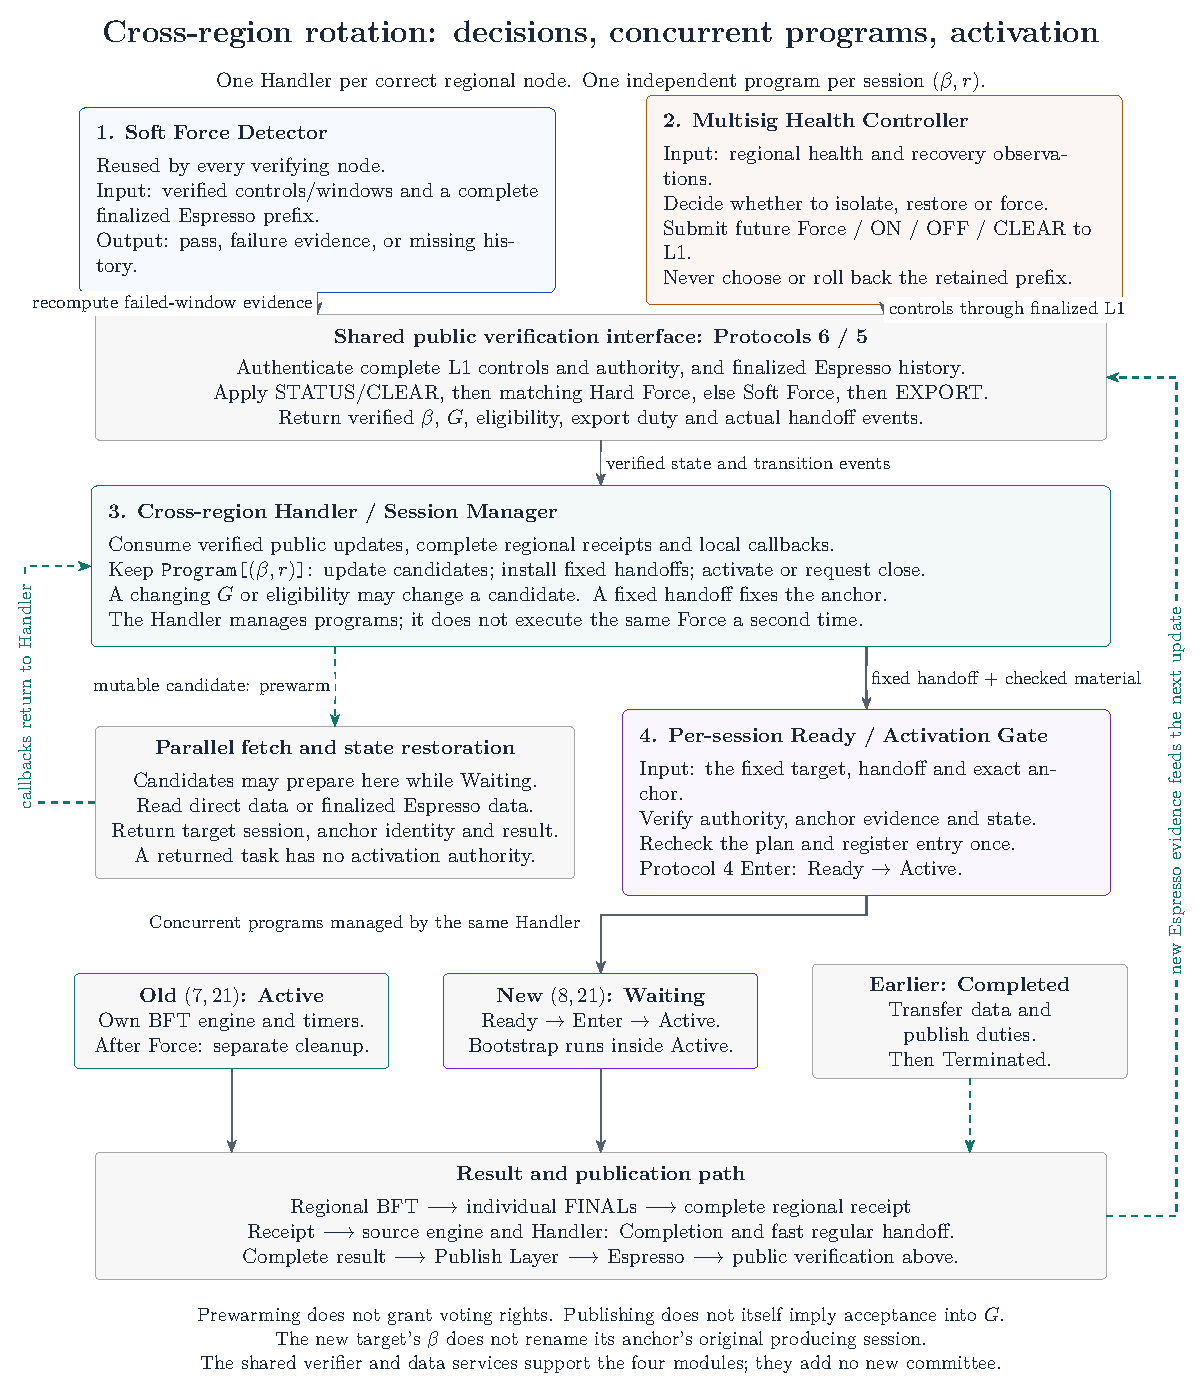
\includegraphics[width=.98\linewidth,height=.87\textheight,keepaspectratio]{figures/cross_region_rotation_v3_2/modules.pdf}
\caption{The four cross-region modules and their shared verification and
publication services. Each regional node manages independent programs;
prewarming and fixed-handoff activation use distinct paths.}
\label{fig:runtime-modules}
\end{figure}
\FloatBarrier

\subsection{Soft detection and multisig health control}
\label{sec:runtime-controls}
The Soft Force Detector takes a validated replay checkpoint and the
complete following Espresso prefix. It reproduces the current export
duty and settles its fixed windows as in \cref{sec:windows}. It returns
either no failure, a failed-window descriptor with its first crossing
header and supporting history, or a need for missing evidence. The
descriptor binds the chain, current branch version, export-session pair,
window start, deadline, target, accepted count, consecutive miss count
and fixed tolerance $M=1+\beta$. A miss below the tolerance does not
authorize Force. Missing namespace or control evidence is never a zero count.

Only DATA actually appended to $G$ counts. Duplicates, DRAIN, proposal
QCs and rejected DATA candidates do not count. Invalid outer hints or
unrelated batch objects do not erase credits of accepted DATA. The observed export session can
lag several speculative production sessions. Polling only supplies new
history; its frequency and local reception time do not decide a failure.
Every recipient recomputes a supplied descriptor against its own
authenticated prefix. Protocol~5 remains the sole Force transition:
independent STATUS/CLEAR, the first matching MSIG, otherwise the
automatic check, then the block's EXPORT payload. A computed soft
condition cannot bypass a matching hard intervention in that prelude.

\subsubsection{Multisignature health policy}
\label{sec:health-policy}
The honest, coordinated committee of \cref{ass:committee} runs the
following signing policy. This restricts which new controls it issues;
honesty alone did not imply these restrictions. Health and operational
reports can request an intervention, but their accuracy or delivery time
is not a premise of the results below. No report, including an emergency
report, bypasses the policy's finite credits.

The policy never changes an issued control's target, activation time or
priority. Every submitted MSIG still reaches the first-crossing check of
\cref{alg:force}: the first due record matching the entry branch version
takes precedence over AUTO, and other due records are consumed as stated
there. A regular handoff does not invalidate its target. No controller
decision postpones a matching MSIG until completion, revokes accepted
DATA, or selects an older retained anchor.

\paragraph{State and credits.}
The controller advances one verified replay cursor monotonically and
retains a durable signing journal across restarts and service replacement.
Let $\kappa$ identify its observed accepted tip by chain, DATA height,
block hash and provenance. For each $\kappa$, three initially unused bits
$f[\kappa],\ell[\kappa],c[\kappa]\in\{0,1\}$ permit at most one MSIG,
one health lease, and one optional CLEAR, respectively. A lease concerns
one region. Let $d_i$ count DATA produced by region $i$ and accepted into
the controller's observed $G$. A further bit $u_i[d_i]\in\{0,1\}$ permits
at most one lease for $i$ at that count. All these bits are initially zero;
using a credit sets its bit to one permanently.

The journal binds each reservation to its exact operation and records
signature release, actual submission, finalization and canonical
processing. It also retains each region's outstanding lease. Every
signing path reserves its credits durably \emph{before} releasing a
signature. Stale targets, failed or uncertain submissions, expiry and
abandoned operations never refund a credit. Retries use the same exact
record and control identity, not a newly signed replacement. If an
operation may never have been submitted, a retry must still satisfy the
advance-announcement condition for a first submission.

Only a newly observed accepted tip provides a new $\kappa$; only newly
accepted DATA from $i$ advances $d_i$. Force, recovery, cooldown, Ready,
raw publication and receipt formation do neither. Re-reading old history
never moves the cursor backwards or resets a bit. In particular, accepted
DATA from another region cannot replenish $u_i$. Missing control or
namespace evidence pauses new signing decisions.

\paragraph{Controller actions.}
Managed regions start with governance flag ON. This module issues only
the following health controls, each under the existing authorization and
advance-announcement rules. An exhausted credit leaves an operational
request unsigned and without public effect.
\begin{enumerate}[label=\textbf{H\arabic*)},itemsep=3pt]
\item \textbf{Interrupt a branch.}
At the verified cursor, if $f[\kappa]=0$, reserve that credit, bind the
observed $\beta$, and submit one future MSIG with \emph{empty attached
configuration}. Choose its timestamp using the actual submission time.
If its target later becomes stale, do not retarget it or refund its
credit. Health exclusion, when requested, uses the separate lease action.

\item \textbf{Lease an OFF status.}
For region $i$, require $\ell[\kappa]=u_i[d_i]=0$ and no outstanding
lease for $i$. Reserve both credits. First submit an independent
STATUS ON$(i)$ at a finite future threshold $\theta_{\rm on}$, and wait
until that exact record is finalized and available. At the proposed
OFF submission time $s_{\rm off}$, choose a threshold satisfying
\[
 s_{\rm off}+T_{\rm L1}+\epsilon_E+\eta
 <\theta_{\rm off}<\theta_{\rm on}.
\]
If no such threshold remains, abandon the OFF before releasing its
signature; keep the pending ON and the spent credits. Otherwise submit
an independent STATUS OFF$(i)$ with activation threshold
$\theta_{\rm off}$. Never issue a
second OFF for this lease. Do not start another lease for $i$ until all
its issued records have been canonically processed and any unissued OFF
has been definitively abandoned. An uncertain submission remains pending.

\item \textbf{Clear a cooldown, optionally.}
The default is to await automatic expiry. To clear it early, require
$c[\kappa]=0$, reserve that credit, and submit one authorized future
CLEAR for the named region. A recovery report or ON does not clear a
cooldown, replenish a credit, or reopen a closed branch.
\end{enumerate}

The lease's ON withdraws temporary exclusion; it does not certify
recovery or future synchrony. Its activation is already scheduled before
OFF can be submitted, so restoration needs no later recovery report or
unsigned controller promise. Sequence order need not equal activation
order. If one Espresso timestamp jump crosses both thresholds, the
independent STATUS records apply OFF and then ON in that prelude; the
lease may have no effective exclusion interval.

Empty attached configuration is material here. A scheduled MSIG with
attached OFF and an independent ON at a later threshold can first become
due in the same block. Then all independent STATUS records run first,
and the MSIG's attached OFF can overwrite that ON. The new policy avoids
this case; it does not reinterpret an older record that contains such
configuration.

\paragraph{Administrative scope and adoption.}
An explicit permanent administrative removal is separate from health
leasing and removes that region from the managed-region service claim.
Before scheduling that OFF, stop new leases for the region and reconcile
its pending health controls; an already issued ON retains its original
effect. Unlimited administrative or emergency signing outside this
module invalidates its finite-intervention guarantee. Such a bypass
cannot be treated as an uncounted benign exception.

The following restoration result concerns execution of this policy from
genesis, with its clean journal and managed flags initialized ON. For
adoption into an existing execution, separately inventory the finite
backlog of reserved, released or submitted legacy operations; preserve
every issued record's original semantics. Its outstanding MSIG count
adds to the bound below. Legacy OFF records need not have restoration
ONs, so restoration is not claimed until they are explicitly reconciled.
In particular, a corrective ON for legacy attached OFF must be submitted
after observing its canonical processing, not merely assigned a later
threshold. No bound on legacy cleanup or controller catch-up is assumed.

\begin{proposition}[Finite controls at a fixed accepted prefix]
\label{prop:finite-controls}
Suppose the actual accepted prefix is a fixed $G^*$ from time $s_0$
onward. Write $h^*=h(G^*)$ and let $h_0\le h^*$ be the controller's
observed accepted height at $s_0$. After $s_0$, it makes at most
$h^*-h_0+1$ new reservations of each of MSIG, health lease and CLEAR.
If $N_0$ previously reserved MSIG operations can still cause a Force,
including operations whose signatures have not yet been released, then
at most
\[
 N_0+h^*-h_0+1
\]
effective MSIG Forces occur after $s_0$.
\end{proposition}
\begin{proof}
The controller's monotone cursor can only visit accepted tips on the
ancestor chain of $G^*$, at heights $h_0,\ldots,h^*$. Each such key has
one credit of each kind. Reservations under earlier keys are already
in the prior journal, and their pending MSIGs are included in $N_0$.
Each issued MSIG has at most one effect under \cref{alg:force}; stale
records and exact retries do not add effects. This also covers delayed
ingestion of already accepted DATA. If $h_0=h^*$, at most one new MSIG
reservation remains, rather than a new credit after each beta change.
\end{proof}

\begin{proposition}[Restoration after finite health exclusion]
\label{prop:health-restoration}
Consider a region that remains managed under the policy from genesis,
and suppose Espresso timestamps keep growing as in \cref{sec:progress}.
If $G$ eventually stops growing, that region eventually has governance
flag ON permanently. The same conclusion holds, even if other regions
continue advancing $G$, whenever this region contributes only finitely
many accepted DATA blocks.
\end{proposition}
\begin{proof}
For a fixed $G$ tail, \cref{prop:finite-controls} leaves only finitely
many lease reservations, including the finite prior journal. Independently,
if region $i$ contributes only finitely many accepted DATA blocks, its
observed counts $d_i$ range over a finite set. Each count permits at most
one lease, irrespective of other regions' progress.

Every issued OFF has a previously finalized independent ON with a finite
later threshold. Growing timestamps eventually cross it. The two records
end in ON even when their first crossings coincide. A later lease for
the same region cannot overlap this processing, and new MSIGs have no
attached status changes. With finitely many leases, the last issued OFF
is therefore eventually undone. A lease abandoned before OFF release
cannot prevent restoration. The initial flag is already ON if no OFF
was issued.
\end{proof}

These are control-policy results. ON still leaves cooldown and authority
checks in the eligibility rule. AUTO may continue to interrupt work, and
global growth may replenish MSIG credits indefinitely. The results do
not establish timely receipt formation, useful service for every region,
or request acceptance. They supply finite committee interference for a
fixed-$G$ argument without strengthening the frozen service conditions
into recurring successful intervals or an accurate failure oracle.


\subsection{Cross-region Handler}
\label{sec:session-manager}
The manager serializes events that modify its local control state.
Data retrieval and state restoration may run concurrently. Its
inputs and outputs have the following meanings.

\begin{table}[htbp]\centering\small
\caption{Session Manager inputs.}
\label{tab:manager-inputs}
\begin{tabularx}{\linewidth}{@{}>{\raggedright\arraybackslash}p{.24\linewidth}Y@{}}\toprule
Event & Validation and routing\\\midrule
\texttt{L1Finalized} & Authenticate the complete control prefix and
authorities; queue future controls without activating them.\\
\texttt{EspressoFinalized} & Authenticate complete ordered history;
consume the state transition produced by \cref{alg:external,alg:force}.\\
\texttt{RegionalFinalized} & Validate the DATA, complete FINAL receipt
and required ancestry; route to the producing pair and offer the result
to the Publish Layer.\\
\texttt{MaterialAvailable} & Check the target pair, anchor's producing
pair, height and hash, requested object and verified result; update only
the matching preparation or fixed handoff.\\
\texttt{CoreEvent} & Accept an event from the named local engine;
record its view, quit, recovery, Completion or retirement progress.\\\bottomrule
\end{tabularx}
\end{table}

The manager retains $\tagg{Closed}[\beta]$ with its authenticated proof
even if it has no program for that version. This is public source evidence,
not a new committee certificate. Program deletion cannot delete the map
or its pending control-routing duties. Before processing a complete
old-session proposal, ReadyBundle, authority packet or archived message,
the dispatcher checks this map. If closure forbids entry or a fresh
action, it serves and relays the full closure using the packet's verified
historical membership context as specified in \cref{sec:retirement}.
Silently dropping the packet is not permitted. This control response
does not sign a BFT vote or revive the terminated engine.

One FINAL signature is not a \texttt{RegionalFinalized} event. Existing
participants collect matching signatures into the receipt of
\cref{def:receipt}. A correct holder delivers the complete result to
the manager and the entered source engine, multicasts the complete
receipt and dependencies to the fixed regional membership, and offers
the complete original publication value to the Publish Layer under
\cref{sec:input-report-carriage}. The source engine applies the existing receipt and Completion
rules. A program that has not entered only caches the result; receipt
arrival cannot create an engine or skip its handoff checks. Aggregation
is not a new consensus round. $T_{\rm pub}$ still starts when a complete
result becomes available.

The outputs are \texttt{Prepare/Fetch}, naming the target and exact
requested material; \texttt{Activate}, invoking Protocol~4 once;
\texttt{RequestClose}, carrying a verified closure cause;
\texttt{OfferResult}, preserving original DATA and receipt fields;
and \texttt{Persist/Release}, recording state and transferring resource
responsibilities. A cached callback is material, not an activation
command. A late result can be useful to storage without matching the
program's current preparation target.

% Version 3.7: retained source bytes and dependency-complete regional processing.
\paragraph{Node-level source retention.}
\label{sec:source-step}
\label{sec:source-retention}
Each correct regional member keeps a durable \tagg{PublicStore} shared
by its source reader, interpreter, manager, engines and publication
workers. It retains content as well as cursors and indexes. The store
has the following distinct components.
\begin{table}[htbp]\centering\small
\begin{tabularx}{\linewidth}{@{}>{\raggedright\arraybackslash}p{.24\linewidth}Y@{}}\toprule
Component & Retained content\\\midrule
Raw Espresso source & Every acquired complete relevant namespace,
including rejected or malformed records; headers, finality/linkage
proofs, authenticated absence, and canonical source order.\\
Object dictionary & Actual object bytes, content commitments,
authenticated source identities and occurrence paths. An index without
the bytes is not a retained object.\\
L1 source objects & Every obtained finalized authority, control,
header and registry/completeness proof, with its authentication inputs;
pending controls as well as applied controls.\\
Regional witnesses & Full validation bundles actually used by correct
regional actions, committed DATA and receipt dependencies. Possession
does not itself make a private object public in an EXPORT.\\
Prepared anchors & Exact executable continuation objects and their
validated provenance, separately keyed by anchor, configuration,
region and native format.\\
Replay state & Verified checkpoint, exact canonical subposition,
pending boundary, source-availability cursors, and typed pending fetches.
The source-availability cursor is distinct from the interpreter cursor.\\\bottomrule
\end{tabularx}
\end{table}

At each source-availability event, retain the entire authenticated raw
namespace and its evidence before advancing the availability cursor,
releasing the input buffer, or making a relay depend on it. Rejection
by P6 never deletes raw evidence. Likewise retain each acquired L1
object before advancing its authority-fetch cursor. Regional validation
retains the witness it used, so a later required complete send does not
reconstruct that witness from an archive. Correct FINAL and complete
receipt sends obey the full-bundle rule of \cref{sec:admission}; a
reference is used only when its receiver can resolve it within the
existing regional delay bound.

Beta replacement, session closure, advancement of $G$, checkpoint
compaction and worker exit do not delete these objects. Cancellation
removes a consumer, not the store's retention responsibility. Transfer
outstanding sends and ownership durably before releasing resources.
Restart restores the exact store and replay subposition; loss of required
bytes requires hydration before the prepared timing claim can resume.
These are protocol storage rules, not an additional storage service.

\paragraph{Finite initial hydration and pruning.}
\label{sec:source-hydration}
Choose a fixed authenticated source cut $q_0$ when beginning this
retention discipline. Hydrate the raw source interval still legally
referenceable after that cut and all exact objects designated by the
starting checkpoint. Under the unrestricted historical-reference rule,
this includes relevant raw namespaces back to the authorized source
origin, including rejected records. Merely retaining accepted ancestry
is insufficient. Also prepare the fixed anchor's provenance and the
finite authority prefix needed by the regional-response argument.
Retain every newly available namespace beyond $q_0$ while hydration
runs. Neither a new beta nor a later source height restarts the fixed
old task or changes its target to a moving cut.

The interval and each admitted payload are finite. Eventual historical
retrieval gives a finite completion time for that fixed set; the anchor
and finite AUTH prefix have their separate eventual-availability
premises. Taking a finite maximum imposes no uniform archive,
authority or native-restoration bound. It does not include all future
L1 objects that an arbitrary sidecar might name.

A replay checkpoint may compact computation without deleting
referenceable bytes. Deduplication and equivalent lossless storage are
allowed while exact content and source-occurrence mappings remain
available to the modeled handler. A hash or an only-eventually-readable
archive is not a replacement for those bytes. Pruning requires a
protocol proof that no future supported reference, checkpoint,
anchor, pending validation or publication duty can need the object.
Advancing $G$ or terminating its producing engine does not prove this.
The present rule supplies no finite-storage bound.

\paragraph{Common public-kernel completeness.}
\label{sec:record-completeness}
For a logical EXPORT at position $p$, the common public basis consists
of its actual objects, the authenticated earlier source objects its
baseline references denote, and the objects established by its
protocol-authorized checkpoint. A private newer checkpoint does not
change this basis. Exact content-identity or source-identity aliases
are resolved under \cref{sec:logical-carrier}; an explicit redundant
occurrence position is not required. The dictionary must establish the
actual object and its permissible source occurrence. An unresolved
sender assertion or a name without a supplied public object cannot
complete a kernel. L1 objects retain their own authentication interface
and need not first occur in Espresso.

The required kernel comprises actual DATA/covering-path bytes, FINAL
signatures, its fixed incoming context, and the source inputs needed
for the independent public gates. An old raw object can be evidence
even if its containing record's DATA was rejected. This never grants
retroactive append permission. A cache hit cannot make a privately
held or genuinely absent object publicly supplied. A cache miss for a
specified legal public object requires retrieval and resumption at the
same position; the prepared retention invariant below rules out such
an Espresso byte miss in the timed cohort.

Check typed identities, actual hashes, the signed domain, current pair
and fixed snapshot before deeper public validation. A false outer base,
version or interval hint is not a gate. Verify FINAL signatures under
that snapshot, then apply \tagg{CheckFINAL} and the actual global gates.
A publisher-selected PROPOSE, recovery $\tagg{AUTH}_{r,g}$ path, L1
reference proof sidecar or unbound native claim is not a kernel input.
Its optional verification cannot delay public replay. The correct
signer's full regional checks justify intrinsic input validity by
\cref{prop:final-kernel-soundness}; they do not justify a new private
public-basis object or an arbitrary sidecar assertion.

An absent required DATA object or invalid signature makes that kernel
incomplete or invalid. Continue with independently complete kernels;
no whole-record validity flag suppresses a valid neighbor. In contrast,
a missing complete namespace, applicable control prefix or genuine
current canonical boundary input pauses that operation. It is never
zero weight or an empty candidate set. Optional regional evidence is
retained and routed to its own engine; a complete genuine Quit retains
its original evidence-first handling, while an incomplete optional
admission path is not a public source dependency.

Terminal DATA's validation and durable commit precede the successor
wait in \tagg{ResolveBoundary}. Packet preparation and whole-record
prechecks cannot invert this order. Save the exact subposition and
expose the accepted prefix before any later boundary wait.

\paragraph{Immediate regional source relay.}
A \tagg{SOURCESTEP} is an authenticated message to an installed fixed
regional snapshot. It carries its chain/protocol domain and sender,
the source height and full header, complete relevant namespace or
absence, finality/linkage evidence and canonical record order. It
identifies the maintained verified predecessor checkpoint, supplies
applicable complete L1 controls and the available fixed-boundary
inputs, and supplies required exact public bytes not already resolvable
by the recipient under the existing complete-message contract. The
recipient never trusts a sender-selected new checkpoint.

On acquiring a complete raw source input, each correct member retains
and sends it in that availability event, before waiting for its own P6
result. Inventory the actual inline and retained source objects without
first fetching the union of all optional witness targets. This relay
need not know which region replay will select. Native preparation does
not delay it. Missing mandatory boundary evidence remains an explicit
wait and is supplied in a later complete dependency event. An initial
raw relay is not falsely described as a complete boundary operation
when that evidence is absent. Equal packets are deduplicated by source
position and commitment without suppressing the first correct relay.

A sender includes full required bytes unless recipient resolution is
already covered by the regional full-bundle contract. Its own cache hit
alone does not justify omitting bytes at a recipient. Acquisition of an
additional exact dependency immediately resumes its saved operation;
there is no independent polling tick or replay job.

\paragraph{Receive, commit and activate.}
The receiver authenticates and retains the input, then processes the
contiguous dependency-complete prefix from its maintained checkpoint.
Out-of-order source inputs wait for their predecessors. For each ready
block it executes P6, including P5, the public-kernel checks and ordered
per-DATA transactions. Each transaction records its accounting,
boundary and subposition and exposes the accepted DATA before any
later wait. A duplicate cannot repeat a committed prelude, count or
boundary. Local receive times do not replace canonical timestamps.

The same complete event delivers the verified transition to the Session
Manager. When the exact anchor continuation and remaining full Ready
inputs are already prepared, the Manager checks the fixed handoff and
live activation predicate and performs Ready/initial Enter once. It
attaches the already executable object; it does not import a database
or reconstruct native state here. No old lock, vote or entry time is
inherited. A Force-created version still cannot export in its triggering
block.

On closure, persist the version-wide \tagg{Closed} gate and control
routing obligations atomically. Every entry, fresh action and callback
checks that gate by its own beta. Worker scans, archive copies and
retirement completion are not prerequisites to gating the old version
or entering a valid new pair. A complete old-session context still
invokes the existing complete-close handler and multicast under
\cref{sec:retirement}, even for Waiting, Completed or Terminated records.
Unresolved snapshot context remains pending. The original per-session
$c_v$, $4\Delta$ drain and evidence duties remain unchanged; recording
\tagg{Closed} alone neither starts that drain clock nor permits exit.

\begin{proposition}[Retained public source bytes]
\label{prop:retained-public-bytes}
After fixed-cut hydration, a continuously online history-following
member that executes the retention rules keeps every legally
referenceable acquired Espresso object and its authentication evidence.
If $J_q$ first becomes final at real time $a$, the required Espresso
bytes through $q$ are available to that member by $a+T_E$, without a
new archive read for a previously acquired object.
\end{proposition}
\begin{proof}
Hydration establishes the claim through the fixed cut. At each later
availability event, insertion of the entire raw namespace precedes the
availability-cursor advance and any rejection. Old aliases resolve to
retained bytes; actual new objects reside in this namespace. An absent
object is not fabricated. No retry, checkpoint or worker transition
removes referenceable content. Induction over source positions preserves
the claim. Every predecessor through $q$ became final no later than $a$,
so the frozen visibility premise supplies its new source bytes and
Espresso evidence by $a+T_E$. Older hydrated bytes remain present.
This is an Espresso-byte assertion, not a deadline for new L1 authorities.
\end{proof}

\paragraph{Prepared regional timing.}
\label{sec:source-step-timing}
Consider the continuously online, hydrated regional members in a tail
with fixed $G^*$ and installed slot $r^*$. The finite required AUTH
prefix, exact anchor provenance and executable continuation have been
prepared and retained. Applicable controls arrive before their
crossings. Public candidate validation requires no new recovery AUTH,
L1-reference sidecar or native-output acquisition: \tagg{CheckFINAL}
uses the fixed initial authority and actual public DATA/FINAL bytes.
\Cref{prop:retained-public-bytes} supplies all required old Espresso
references, including ones in rejected records. The dependency case
split in \cref{prop:v35-public-response} checks every operation preceding
the first positive DATA.

Let $J_q$ open a retry for region $i$ and first become final at time
$a$. Its required source inputs are present by $a+T_E$. The immediate
regional send and complete receive handler finish by
$a+T_E+\Delta_i$. If the pair remains activatable, the Manager's final
step attaches its prepared state and enters, so
\[
 e(\beta,r,0,0)\le a+T_E+\Delta_i.
\]
A verified intervening closure supplies the other outcome. Ready uses
the opening header and needs no subsequently generated empty block.

The charged complete-message operation consists of envelope/source
checks, lookup of resident exact bytes, logical inventory and public
kernel validation, canonical prelude and DATA accounting, durable cursor
updates and the guarded attachment of already executable state. It uses
the existing regional complete-message interpretation for the maintained
input path under its admitted input/load limits. There is no separately
scheduled native replay or external fetch inside that operation.
Finiteness alone does not bound an arbitrary CPU computation or historical
backlog; calling a task atomic does not create such a bound. A concrete
adapter must implement this interface. Physical database import, external
archive reads and returning-node catch-up must finish before invoking
it. No $\Delta_i$ application-processing deadline is asserted for an
arbitrary external observer, which receives no such regional relay.
The rule adds no service premise, public READY certificate or new
publication obligation.


\begin{protocol}[H]{alg:rotation}{Handle cross-region events and manage sessions}
Each correct regional replica runs this handler independently.
\begin{enumerate}[label=\textbf{\arabic*)},itemsep=3pt]
\item \textbf{Validate the event.} Route authenticated public input,
regional results and local callbacks by their stated context. Preserve
pending requests and source evidence. Reject a purported completion
whose material or session does not match its request.
\item \textbf{Consume public replay.} For new public history, run or
consume \cref{alg:external}, including \cref{alg:force} in its canonical
order. Use its resulting $\beta$, $G$, eligibility snapshots, duty and
boundary records. This handler never increments $\beta$, chooses a
different cutoff or modifies $G$ independently.
\item \textbf{Reconcile handoffs.} From valid terminal receipts,
derive regular boundaries while their version remains open. Consume
fixed Force boundaries from replay. Verify them by
\cref{sec:witness}. Prepare selected local targets; send complete
handoff material to the selected members when available. A future
Force does not block a current regular handoff.
\item \textbf{Reconcile candidates.} Recompute possible future
targets from the current export context, $G$, eligible regions and
known future controls. Update only unfixed preparations. A different
target pair uses a different record. Pause obsolete speculative work;
terminate an unentered program only when verified facts make that
target impossible or assign its fixed handoff to another region.
\item \textbf{Handle closure and results.} Store every verified closure
in the manager's durable $\tagg{Closed}[\beta]$ map. Gate new entry and
fresh actions regardless of phase. For each known session snapshot in
that version, including unentered and archived programs, run the complete
closure relay and idempotent \texttt{RequestClose} of \cref{sec:retirement}.
If the snapshot is not yet known, retain a pending relay obligation.
Any later old-session packet with the necessary context triggers this
control response before ordinary processing. Keep signed routing,
historical evidence and publication duties. Apply terminal receipts
to entered source engines under the existing Completion rule.
\item \textbf{Check and enter.} For each selected local Waiting
program with a fixed handoff, check \cref{def:ready}. In the same local
event, recheck public validity and the durable entry flag, record Ready,
and invoke Protocol~4 Enter atomically. A failed check leaves Waiting
or applies a justified cancellation; it does not partially initialize
the engine.
\item \textbf{Persist and dispatch.} Durably record state changes,
entry and exit records, and required outgoing actions before exposing
them. Dispatch asynchronous work with its full target and anchor
context. Repeated events resume outstanding actions without creating
another logical entry.
\end{enumerate}
\end{protocol}

The public interpreter has one mutation path: Protocol~5 defines
control, window and Force transitions; Protocol~6 authenticates and
applies them and accepts DATA from EXPORTs. Protocol~3 consumes those results.
Protocols~1 and~2 update only the named session's regional core.
An implementation may place these modules in one process without
changing this division of authority.

\subsection{Session lifecycle}
\label{sec:session-lifecycle}
The manager maintains the following record for each local program:
\[
\begin{aligned}
\tagg{Program}[\beta,r]=(&\mathit{phase},\mathit{preparing\_plan},
 \mathit{fixed\_handoff},\mathit{anchor\_block},\\
 &\mathit{execution\_state},\mathit{authority\_and\_bounds},
 \mathit{core\_state},\mathit{pending\_fetches},\\
 &\mathit{entered},\mathit{close\_requested},\mathit{closure\_evidence},\\
 &c_v,d_v,\mathit{publication\_and\_retention\_handles}).
\end{aligned}
\]
The six phases describe the local program, not public finality.
\begin{description}[style=nextline,leftmargin=1.5em,labelindent=0pt,labelwidth=1.5em]
\item[Waiting.] The program is preparing a possible or selected
handoff. It may fetch data, recover state and cache evidence. It has
not entered its regional engine, signed a regional vote or started
a regional commit or progress timer.
\item[Ready.] A fixed handoff, its exact anchor state and all entry
dependencies have passed the gate below. Enter follows in the same
serialized event; Ready introduces no extra scheduling delay.
\item[Active.] The program has entered an unfrozen regional
generation. Initial STATUS, the $2\Delta$ wait, NEWVIEW and ANCHOR
certification all occur in Active. The core runs Protocols~1 and~2,
subject only to the explicit retirement interface in
\cref{sec:retirement} when closure is requested.
\item[Frozen.] The current generation has a valid Quit proof.
The original evidence, receipt and recovery rules apply. Force alone
does not establish a Quit proof or cause this phase.
\item[Completed.] The entered engine has obtained a valid terminal
receipt and performed the original Completion action. It has stopped
regional production and cancelled timers as specified there. Data
delivery and retention responsibilities may remain.
\item[Terminated.] The logical program has exited. It processes no
BFT timer and issues no BFT signature. Durable storage and publication
workers retain its required evidence and duties. An exit record prevents
late messages from restarting it.
\end{description}

Normal transitions are Waiting to Ready to Active; Active to Frozen
on Quit; Frozen to Active on the original recovery admission, with
$g$ advanced and $t=0$; and Active or Frozen to Completed on terminal
Completion. Waiting or Ready may terminate when their target is
definitively invalid. Completed may terminate after responsibility
transfer; if RequestClose began while Active or Frozen, the original
drain deadline still applies. Active or Frozen may terminate only through the retirement
contract in \cref{sec:retirement}. While close is pending, they retain
their core phase and set \texttt{close\_requested}; there is no seventh
phase.

An unfixed \texttt{preparing\_plan} can change when $G$, the source
duty or candidate eligibility changes. The fixed handoff cannot.
Its target pair, assigned region, initial anchor, source context,
selection position, authority and reference bounds remain immutable.
In particular, a later OFF does not replace a historical regular
selection. Local locks, votes, view entry times and timers belong to
one pair only. Recovering a crashed process resumes this durable
logical record; it does not clear its votes or perform another initial
Enter. Storage and task references carry the full pair and anchor
identity. No additional protocol-level session identifier is needed.

Several regions may hold unfixed Waiting preparations for the same
future pair. Only the region selected by the fixed handoff can enter.
Temporary loss of candidate eligibility may pause work without
terminating a preparation that could become eligible again. A retired
record remains a tombstone even after active resources are released.

\paragraph{Shared preparation survives a retry.}
The manager keeps a shared preparation cache keyed by anchor producing
pair/hash, native-state format, configuration and region. A program's
cancellation removes its consumer, not already verified native state
or useful unfinished preparation for the same anchor. No consensus
signature, timer or lock is shared through this cache. The node-level
full-byte public evidence store of \cref{sec:source-retention} is likewise
independent of consumers: beta changes, advancing $G$, and worker exit
do not delete its referenceable raw history or transfer it to an
only-eventually-accessible archive.

It also keeps $\tagg{AuthCache}[r,g]$ and a background sequential fetch
task for the active slot. The task obtains and validates each next
immutable recovery authority, retains it, and advances its fetch cursor.
A beta change does not reset that cursor, drop a future authority
already learned, or cancel the fixed-slot task. Correct regional
members relay complete authority evidence. When the slot remains
fixed, every finite required authority prefix is eventually cached.
This cursor fetches evidence only; it neither enters a generation nor
substitutes a leader. A new engine still starts from $g=t=0$ and uses
its own new-pair admission and recovery proofs.

An Active old program may already lack permission to extend $G$.
A Completed or Terminated program's existing results may still be
accepted if their version and interval satisfy the public acceptance
rules. The phase does not revoke or create that permission.

\subsection{Handoff records, anchors and Ready}
\label{sec:witness}
$\tagg{NextLive}(i,\chi)$ searches the other eligible regions after $i$
in the fixed cyclic order $\mathcal L_R$, then returns $i$ itself if
there is no eligible alternative and $i$ is eligible. Otherwise it
returns $\bot$. Every call uses the designated target authority.
Eligibility still means governance ON, expired cooldown and positive
weight under that authority. A synthetic source $\bot$ searches the
whole list from its beginning.

For Force only, $\tagg{NextOwed}(i,\chi,\mathcal O)$ performs that search
within the public owed set $\mathcal O$ of \cref{sec:owed}. Ordinary
REGULAR selection uses unrestricted NextLive. A physical region may
renew, but the new pair always receives fresh locks, votes and timers.
The conditional AUTO cooldown of Protocol~5 is applied only when another
eligible Force candidate exists. It does not erase an old cooldown or
override OFF.

\paragraph{The target slot of a Force.}
\label{sec:retry-slot}
For an assigned export duty, let $(\beta_b,r_b)$ and $i_b$ be its
producing context, and let $a_b$ be its accepted DATA count so far.
This is accepted count in that duty, not its regional height or number
of raw publications. The target slot is
\[
 r'=
 \begin{cases}
 r_b,&a_b=0,\\
 r_b+1,&a_b>0.
 \end{cases}
\]
The first case is a retry using the same immutable authority namespace.
The second starts a new slot after actual global progress. Both change
the version to $\beta+1$ and start their new engine at $g=t=0$.
The retained anchor is exactly pre-payload $G$, with its original
producing pair, height, hash and commitment evidence.

An unassigned boundary stores both its source context and its already
determined target slot. A later Force changes beta and the cause but
keeps that target slot; it does not infer it afresh as $r_b+1$.
A normal boundary stores source $(i_b,\beta_b,r_b)$ and target $r_b+1$.
Genesis stores source $(\bot,\bot,-1)$ and target 0. This covers repeated
Forces before any new duty is assigned without creating empty sessions.

Normal completion still opens $(\beta,r+1)$ from exactly
$T_{\beta,r}$. A zero-output retry may reuse numeric $r$, including at
another physical region, but cannot rebind $\tagg{AUTH}_{r,g}$.
For a fixed region and $(r,g,t)$, the recorded leader is independent
of beta; beta separates message and engine identities, not the schedule.
The existing fixed snapshot and quota remain those of the record.
No old Quit, vote, lock or timer becomes a new engine's state.

\paragraph{Historical selection.}
For a REGULAR boundary use
\[
 q_0=\max\{\operatorname{height}(\xi(T_{\beta,r})),
                         q^{\rm open}_{\beta,r}+1\}.
\]
For a Force use its triggering Espresso height. Select the first
verified historical position at or above this lower bound for which
the relevant selector returns a region. REGULAR uses
$\tagg{NextLive}(i_b,\chi_E(q))$; Force uses
$\tagg{NextOwed}(i_b,\chi_E(q),\mathcal O_E(q))$.
The pre-payload snapshots are immutable replay products. The selected
height $q_s$ fixes the region and opening reference bound. Missing
source or designated-authority evidence causes a wait, not a skipped
candidate or a fabricated empty set.

The terminal DATA itself need not be globally confirmed to perform
REGULAR handoff. Any suitable later finalized header suffices; it can
be empty or carry unrelated records. If none exists yet, the current
session can still form and offer its terminal result using its already
known opening header. The existing publication service then supplies
a later block. The current Ready gate never waits for this future header.

If the terminal result's own containing block is the first possible
selection position, that terminal DATA can be accepted while the
successor opens there. The successor's DATA cannot be in that same
EXPORT: its minimum reference would equal the containing block.
Multi-session EXPORTs remain possible when the successor was already
selected at an earlier finalized position. Speculative regular handoff
does not update the public owed ledger.

\paragraph{Typed handoff packet.}
A handoff packet contains the fields below. References can name
authenticated cached objects or objects still to be fetched; a reference
alone does not establish Ready.
\begin{table}[htbp]\centering\small
\caption{Handoff packet fields.}
\label{tab:handoff-packet}
\begin{tabularx}{\linewidth}{@{}>{\raggedright\arraybackslash}p{.26\linewidth}Y@{}}\toprule
Field & Type and meaning\\\midrule
Domain and kind & Chain/protocol domain; one of REGULAR, MSIG, AUTO.\\
Source context & Predecessor pair $(\beta_b,r_b)$ and source region
$i_b$, including the accepted count when assigned and the stored target
slot when unassigned.\\
Target & Target pair $(\beta',r')$, the retry/new-slot reason and selected
region $i_{\rm next}$.\\
Anchor & Producing pair, DATA height, hash, full DATA or reference,
and original direct or covering commitment evidence.\\
Authority & Finalized $\tagg{AUTH}_{r',0}$, its fixed configuration,
quota, and publication-height proof.\\
Selection and bounds & $q_0,q_s$, authenticated eligibility and,
for Force, owed-set snapshot,
$q^{\rm open}_{\beta',r'}$ and $\lambda^{\rm open}_{\beta',r'}$.\\
Cause and evidence & Mode-specific cause; trusted or validated replay
checkpoint, complete required L1/Espresso history and regional proofs.\\\bottomrule
\end{tabularx}
\end{table}

\paragraph{Handoff verification.}
\label{sec:verify-handoff}
The pure procedure $\tagg{VerifyHandoffHistory}(C,\mathcal H,P)$ takes an
authorized replay checkpoint $C$, required source history $\mathcal H$
and packet $P$. It returns historical fixed fields, invalid, or needs
evidence. It authenticates what the boundary established; it does not
require its version to remain open now and grants no entry permission.
A separate activation predicate is given after the procedure. Neither
procedure changes public replay.
\begin{enumerate}[label=(\roman*),itemsep=2pt]
\item Check the domain, field types, source and target names. Replay
authenticated compatible history from $C$ through all positions
needed by the cause, historical selection and incoming boundaries.
Verify complete applicable controls, not only inclusion of the named
control. Consult validated caches when available. Historical receipts
from a producing session can use \tagg{CheckFINAL} for intrinsic input
validity; this external check does not fetch that producer's optional
recovery-admission path. It still authenticates each fixed initial
snapshot and exact DATA ancestry. The target's executable state and
fresh regional admission remain separately verified.
\item For REGULAR, validate the predecessor's own fixed boundary,
initial authority, exact quota and terminal DATA
$h(T_{\beta_b,r_b})=h(A_{\beta_b,r_b,0,0})+\TB_{r_b}$.
Validate its terminal FINAL kernel, actual ancestry and signed $\xi$,
including the independent historical source and boundary checks.
Require $\beta'=\beta_b$ and $r'=r_b+1$. The anchor must equal the
terminal DATA. Recursively validate the predecessor boundary in this same
historical mode; current closure does not erase its original evidence.
\item For MSIG, verify its authorized finalized L1 record, control
sequence and first-crossing header $J_{q(\theta_a)}$. Replay the
entire prelude and check that this is the first due Force whose target
matches the entry version. Check attached changes only under this
match. A stale instruction or another due instruction consumed by the
same prelude cannot form a second boundary.
\item For AUTO, replay the fixed base windows, consecutive miss count
and the duty's tolerance $M=1+\beta$. Check that the triggering prelude
is the first crossing at which the miss threshold is reached, and that
no matching higher-priority MSIG applies. Recompute the conditional
cooldown and its eligible alternative using the target authority and
owed snapshot. One missed window below $M$ is not a Force; an alarm or
local timeout is not proof.
\item For either Force, obtain the captured source context, old and
new versions, retained prefix and boundary from that unique replay
transition. Require $\beta'=\beta_{\rm entry}+1$, the target slot
derived in \cref{sec:retry-slot}, and anchor equality with pre-payload
$G$, including prefix provenance. Verify zero or positive accepted count
rather than inferring it from the anchor's producer.
During an unassigned interval, verify the stored context and any
intervening Forces rather than inventing an empty export session.
A later Force supersedes this boundary for future activation, but does
not invalidate its historical cause, original selection or retained anchor.
\item Recompute the first eligible $q_s$ from $q_0$ and all required
historical snapshots. Use unrestricted NextLive for REGULAR and
NextOwed for Force. Check the target region and immutable target authority.
Set $q^{\rm open}_{\beta',r'}=q_s$ and
$\lambda^{\rm open}_{\beta',r'}$ to the maximum of the anchor's L1
reference height and the initial authority's publication height.
Validate the anchor's original direct or covering commitment evidence
under \cref{sec:coverage,sec:receipt-kernel}, its complete block and
required ancestry.
Do not relabel it with the target pair.
\item Compare the derived fixed fields with $P$ and any existing
fixed record for its target pair. Equal duplicates share that record;
different fixed fields for the same pair are rejected. A packet cannot
replace an already installed handoff. This step records historical facts,
not a claim that the target may still enter.
\end{enumerate}

\paragraph{Permission to enter now.}
\label{sec:can-enter}
$\tagg{CanEnter}(S,P)$ takes the manager's current verified public state
$S$ and a packet whose historical check has passed. It requires that the
target version is current and open, the packet is the still-applicable
fixed boundary, this replica's region is selected, and the local record
has no prior initial entry, close request or Terminated record, and the
manager has no authenticated $\tagg{Closed}[\beta]$ for that target.
A Closed record blocks entry even before a complete per-session $c_v$
can be set; context resolution and closure relay still run before refusal. Ready
also checks the exact anchor state and dependencies below. A duplicate
already-entered record can be serviced without another Enter.

All initial entry paths use both predicates. Receipt, ancestry and
retained-anchor validation use historical validation only, and global
EXPORT acceptance independently checks its current append permission.
For example, after Force closes version 7, the original boundary and
receipt for retained DATA 108 of $(7,20)$ remain valid history.
$\tagg{CanEnter}$ rejects reopening $(7,20)$, while a valid new Force
packet may inherit that same DATA in $(8,21)$. A cache miss follows the
same historical checks as a cache hit; no prior cached verdict is assumed.

A Force without an eligible successor still has a fixed cause,
anchor, source context and new version. The interpreter retains that
pending boundary. It has no complete selected packet and cannot make
a program Ready until the first eligible historical position fixes
the target region. A later Force can supersede it while preserving the
same stored predecessor context. The synthetic genesis boundary is
verified against the initial checkpoint and selection rule of
\cref{sec:l1}; it does not claim a nonexistent REGULAR, MSIG or AUTO
cause.

\begin{definition}[\defterm{Ready}]
\label{def:ready}
A local Waiting program for $(\beta,r)$ is Ready precisely when:
\begin{enumerate}[label=(\roman*)]
\item historical handoff verification fixes this target pair and selects the
replica's region, or the authenticated genesis rule does so; the separate
current-activation predicate also passes;
\item its exact anchor's original producing pair, height, hash,
complete DATA and commitment evidence have been validated;
\item the native execution state needed to continue after this
anchor has been recovered and verified against that same anchor;
\item the matching finalized authority, fixed quota, separate
reference lower bounds, the opening Espresso header and all validation
dependencies are available. A header after the opening is not required;
\item the manager's processed public history has not closed or
superseded the handoff; and
\item the durable record has never performed initial Enter and has
no Terminated tombstone.
\end{enumerate}
\end{definition}

State recovery uses the existing native validation interface. Cached state
for DATA 110 cannot make a program anchored at 112 Ready. A future Force
announcement still permits only Waiting/preparation. The complete regional
message interface below states exactly what is relayed and what its
receiver can conclude.

% Version 3.5: current opening header suffices; source-step relay is separate. Insert beside sec:ready; no protocol renumbering.
% This fragment does not redefine def:ready or alg:bootstrap.
\paragraph{A complete regional ReadyBundle.}
\label{sec:ready-bundle}
The following is a proposed message interface for the relay used in
\cref{sec:ready}. It makes the transferred state explicit. It is not
a new READY certificate and does not change the public opening of an
export duty. Its timing claim has the precise scope stated below and
requires independent review.

For target session $(\beta,r)$, let $A=A_{\beta,r,0,0}$ and
$\Delta=\Delta_{i_{\beta,r}}$. A \tagg{READYBUNDLE} is an authenticated
regional message with the following typed fields. Every required object
is present as bytes, once, in its normalized dependency set. A URL,
state root, unresolved hash or promise to fetch later is not a substitute.
\begin{table}[htbp]\centering\small
\begin{tabularx}{\linewidth}{@{}>{\raggedright\arraybackslash}p{.25\linewidth}Y@{}}\toprule
Field & Required value\\\midrule
Domain and target & Chain and protocol domain, encoding/native-state
format identifier, target $(\beta,r)$, selected region and sender identity.\\
Fixed handoff & The complete handoff of \cref{sec:witness}, including
its cause, predecessor/source context, selection and fixed target.\\
Exact anchor & $A$'s original producing pair, height, hash, full DATA,
original direct or covering commitment evidence and required ancestry.\\
Executable state $S_A$ & The full, already constructed application-state
object from which execution after $A$ can continue. It includes all state,
code and continuation metadata required by the native execution interface;
if partial execution is supported, its exact continuation position is
included. It contains no imported regional locks, votes or entry timers.\\
State evidence $\Pi_A$ & Native validation evidence connecting this exact
$S_A$ to this exact $A$, with all proof inputs and dependencies. Use the
existing sound application-validation interface; a sender's assertion
or a bare state hash is insufficient.\\
Authority and bounds & Finalized $\tagg{AUTH}_{r,0}$, fixed configuration
and quota, $Q^0_{\beta,r}$, $q^{\rm open}_{\beta,r}$ and
$\lambda^{\rm open}_{\beta,r}$, and all authority evidence needed to
validate the inherited history.\\
Public evidence & An authorized replay checkpoint and complete finalized
L1 control/authority and Espresso header/namespace histories needed to
verify the handoff, references and supplied authorization context. The
checkpoint's trust/authorization dependencies are included. The packet contains the finalized opening header and its evidence.
It need not contain a header after the opening; the successor selection
floor advances only after the current terminal result forms.\\
Dependency set & Full bytes for the preceding fields' transitive
validation dependencies. A receiver need not fetch an object, replay
application execution to reconstruct $S_A$, or obtain a new authority
before processing this bundle.\\\bottomrule
\end{tabularx}
\end{table}

The native interface determines how $\Pi_A$ verifies state at $A$.
If the block format does not directly commit to a state root, the
bundle supplies the execution evidence and authenticated starting state
required by that interface; this contract does not invent such a
commitment. A merely serialized snapshot that still needs restoration
or conversion is not yet the directly executable state required here.
Recipients independently validate the packet. They do not trust the
sender to authorize a handoff or assert state correctness.

\paragraph{Send and receive events.}
Each correct selected member constructs its complete bundle before its
first Ready/Enter event for this pair. Gathering histories, cross-region
fetching, state reconstruction and bundle formation precede that event;
the existing model assigns them no fixed time bound. At the event it
installs its verified state and executes the existing initial Enter
once, and sends the complete bundle to every member of the fixed
selected-region snapshot. Every correct member does this at its own
first event, so the first correct entrant necessarily sends without
having to know that it is first. Bundle construction or asynchronous
dispatch is not deferred until after the recorded entry time.

The receiver processes the bundle through its serialized Session Manager:
\begin{enumerate}[label=(\roman*),itemsep=2pt]
\item Authenticate the domain, sender and target, and inspect supplied
evidence under the existing evidence-first rule. Validate the historical
handoff, exact anchor, all required authorities, references and native
state evidence. Incomplete or invalid material does not authorize entry.
An existing compatible cache can eliminate duplicate validation, but the
sender does not rely on an unknown receiver cache to omit required bytes.
\item Apply the existing live-activation check against the receiver's
processed public state. A closed or superseded target, a conflicting fixed
handoff, a close request or an exit record prevents initial Enter. This
packet cannot replace a fixed anchor or override newer verified closure.
If the target is closed, invoke the manager's phase-independent closure
relay using this complete packet's verified historical snapshot before
refusing entry. This also applies at a Terminated record and after restart;
the worker need not be recreated. If the same pair already entered,
retain useful evidence without resetting
its state or entry time.
\item For an unentered valid target, validate and adopt the received
$S_A$, check every remaining condition of \cref{def:ready}, then execute
the existing Ready/Enter step of \cref{alg:bootstrap} in this same
message-processing event. The durable entry flag, fixed state attachment
and entry time are recorded atomically before signatures are dispatched.
Relay the complete bundle as above. No separate Ready queue, state-fetch
task or post-Ready installation job lies between this event and Enter.
\end{enumerate}

Here \emph{adopt} has a specific logical meaning: the validated received
state object becomes this new program's executable application state.
The program operates on that object; it does not first reconstruct a
different database from it. This is a representation and message-handler
contract, not a claim that arbitrary database import, disk copying or
native-runtime initialization takes zero time. No receiver can pass Ready
while required installation work remains unfinished.

\paragraph{The exact timing implication.}
Let $e$ be the first correct initial Enter time for this pair. The send
rule places a complete correct-to-correct bundle send at $e$. Suppose the
fixed handoff remains activatable throughout the interval in question
and no closure or other valid entry prohibition intervenes.
If validation, adoption and the atomic Enter transition are the complete
message-processing operation covered by \cref{ass:network}, then
\[
 e_v(\beta,r,0,0)\le e+\Delta
 \qquad\text{for every correct selected member }v.
\]
Indeed, the first correct sender supplies the full executable object and
all validation dependencies. By the existing delivery-and-processing
bound, each correct recipient finishes that handler by $e+\Delta$.
Its guarded final step is Enter, or it has already entered earlier.
There is no remaining state-restoration premise in this argument.

This is the supported abstract-message interpretation, not an additional
service bound for state installation. The quoted network premise covers
delivery and processing of complete validation dependencies. It does not,
by itself, bound an external native import or storage operation merely
because the protocol calls that operation ``installation.'' If such work
remains after bounded message validation, let $u_v\ge0$ be its actual
residual delay. The available decomposition is only
\[
 e_v(\beta,r,0,0)\le e+\Delta+u_v,
\]
when entry eventually completes and remains authorized; the frozen model
gives no uniform bound on $u_v$. Calling that work one event cannot prove
$u_v=0$. In that implementation, the $e+\Delta$ claim and the bootstrap
bounds derived from it remain unsupported.

Consequently the message contract repairs the missing protocol interface
at the abstract level only when the native state is genuinely an executable
validation dependency adopted by the modeled handler. A concrete native
adapter must demonstrate that it meets this contract; sound state proofs
alone do not demonstrate a timing property. The document must withhold
an unconditional native-installation claim until that obligation is met.
No claim is made about an arbitrary history catch-up outside the complete
packet or about when any member first constructs such a packet.

ReadyBundle is regional transport of existing state and evidence. It does
not add a quorum of READY signatures, an Espresso transaction, a publisher
guarantee or a public activation certificate. It neither starts nor resets
an export window. The public clock and the separate live-activation checks
remain those of \cref{alg:force,alg:external,sec:ready}.


\subsection{Activation and bootstrap}
\label{sec:ready}
\begin{protocol}[H]{alg:bootstrap}{Enter and bootstrap the selected session}
Replica $v\in V_{i_{\beta,r}}$ runs these steps for one fixed target
$(\beta,r)$. Let $\Delta=\Delta_{i_{\beta,r}}$.
\begin{enumerate}[label=\textbf{\arabic*)},itemsep=3pt]
\item \textbf{Enter.} In the Ready event, atomically recheck
$\tagg{CanEnter}$ and the manager's Closed map, then check and set
the durable initial-entry flag. Install $A_{\beta,r,0,0}$,
$\tagg{AUTH}_{r,0}$, $\TB_r$ and both opening reference bounds.
Set the entry lock to $Q^0_{\beta,r}$. Enter $(\beta,r,0,0)$
unfrozen, change Ready to Active, record $e_v(\beta,r,0,0)$ once,
and start the original progress checks. Send STATUS with this lock
and the fixed handoff to the initial leader, and process buffered
proofs for this session. Persist entry before dispatching signatures.
\item \textbf{Declare the fixed anchor.} The initial leader waits
$2\Delta$ from its own entry. If the view remains current and
unfrozen and the retirement contract permits the action, send NEWVIEW
choosing exactly $A_{\beta,r,0,0}$, justified by $Q^0_{\beta,r}$
and the fixed handoff.
\item \textbf{Certify and produce.} Members apply the original
ANCHOR-vote step of \cref{alg:recovery}. On the ANCHOR QC, the leader
starts \cref{alg:steady} at DATA height $h(A_{\beta,r,0,0})+1$
and physical position 1. Local failures use the same recovery rules.
All these steps occur in Active, except when the original Quit,
Completion or explicit retirement transition intervenes.
\end{enumerate}
\end{protocol}

Let $e=\min_v e_v(\beta,r,0,0)$ over correct members. Under the
complete-handler timing contract just stated, if the handoff remains
activatable and bootstrap is not interrupted, all correct members enter
by $e+\Delta$. With a correct initializer and no Quit, NEWVIEW is sent
by $e+3\Delta$, its ANCHOR QC reaches the leader by $e+5\Delta$, and
first DATA reaches all correct members by $e+6\Delta$. These bounds
start at first actual Enter, not at public assignment or candidate creation.
If native installation remains outside bounded message processing, these
bounds have not been established; the extra delay is not silently absorbed
into $\Delta$. No public deadline is reset by either implementation.

\paragraph{The public export clock.}
Public replay assigns an export duty independently of a member's
phase. Its window starts at the containing EXPORT's timestamp for
an already selectable normal successor, at the triggering block's
timestamp for an immediately selected forced successor, or at the
first eligible selection block when the boundary previously had no
assigned duty. A selected program may still be Waiting while that
public window runs. Download completion, Ready, process restart and
duplicate handoffs never reset its deadline. Only an unassigned duty
has no DATA window. Missing evidence pauses replay at its canonical
position; it does not create a later public opening time.

\subsection{Concurrent candidates and races}
\label{sec:runtime-races}
Suppose A's session is $(7,20)$ with terminal DATA 110, B already
produces in $(7,21)$, and $G$ ends at 108. A future MSIG targets
version 7. B can retain its old Active program while preparing
candidate $(8,21)$ from 108. If $G$ advances to 109, that preparation
can change to 109; the old Active program's initial anchor remains
110. If Force then fixes B as successor with anchor 109, all further
preparation is for that fixed anchor. B can enter $(8,21,0,0)$ while
$(7,21)$ closes under \cref{sec:retirement}. Their locks, votes,
entry times and timers are distinct.

If A's terminal 110 enters $G$ before Force, the export context
advances to B's $(7,21)$ with zero accepted B DATA. The candidate region
moves after B, but the retry target is still $(8,21)$. With cyclic order
A, B, C, D and the relevant regions owed, C is that candidate. An effective
OFF(C) can redirect the unfixed candidate to D without changing its slot.
Once B's DATA enters $G$, the positive-output rule changes the candidate
slot to 22. If Force finally retains B's 112, its fixed target is D's
$(8,22)$ with original anchor producer $(7,21)$. D must verify state at
112 and authority 22 before starting DATA 113.
Earlier preparation of $(8,21)$ or of state at 109 grants no entry.
OFF cannot rewrite an already fixed regular handoff.

A terminal receipt received before Force can prepare or start a
regular successor in the old version. Once the same node verifies
Force, it cancels an invalid unentered target or requests retirement
of the entered one. If Force arrives first, the late receipt is
retained as regional evidence and cannot resurrect the closed target.
Nodes can briefly have different speculative programs; the same
canonical replay subposition with complete applicable evidence fixes
the same applied public result and Force boundary. Local caches and
future control queues need not agree.

Every fetch callback retains its original target and anchor identity.
A reply for $(7,21)$ at 110 cannot make $(8,21)$ at 108 Ready.
An old candidate reply may be cached and independently validated for
another use, but it cannot overwrite a fixed anchor. Duplicate receipts,
packets and callbacks cannot run initial Enter twice. A stale MSIG
following an earlier AUTO neither closes the new version nor applies
its attached configuration. Reconciliation discards its obsolete
preparation basis without invalidating a different fixed handoff.


\begin{figure}[p]\centering
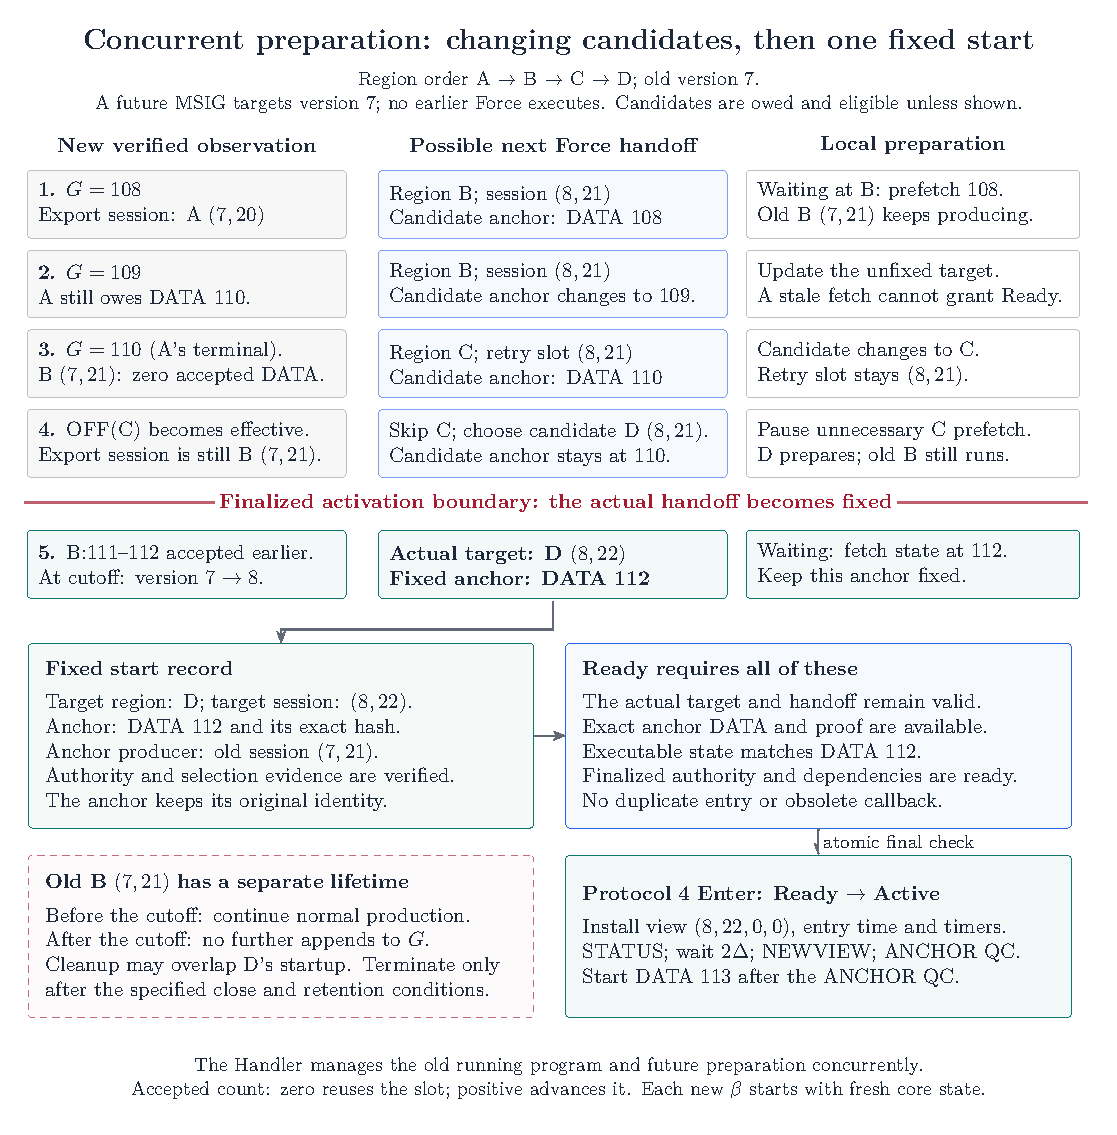
\includegraphics[width=.98\linewidth,height=.87\textheight,keepaspectratio]{figures/cross_region_rotation_v3_5/candidate_ready.pdf}
\caption{A changing Force candidate while the old program continues.
The finalized boundary fixes the target and exact anchor; only then can
verified state at that anchor enable Ready and Enter.}
\label{fig:runtime-candidates}
\end{figure}
\FloatBarrier

\subsection{Graceful close and termination}
\label{sec:runtime-close}
Public closure and program exit are separate events. Protocol~5
immediately removes a closed version's permission for new global
appends. Protocol~3 stores the verified closure and runs its manager-level
dissemination for every known session snapshot, regardless of program
phase. Entered programs also drain through \texttt{RequestClose}. The request is
idempotent and records \texttt{close\_requested}; it is neither Quit
nor terminal Completion. The exact restrictions on new work, treatment
of existing timers and messages, and admissible \texttt{FinishClose}
condition are defined by \cref{sec:retirement}. The drain threshold is derived from the existing regional bound;
resource transfer has no new time bound. A new
session need not wait for the old program to finish closing.

For an unentered program, definitive invalidation cancels pending
entry and can release preparation tasks after the durable closure,
pending-relay and late-message duties have transferred. It has no
regional timers or votes to drain, but it must not stop the manager's
closure dissemination. For Completed, the original Completion action has
already stopped the core. For an Active or Frozen program, only the
retirement contract can authorize \texttt{FinishClose}. An empty local
timer list, a different current public version, or a locally observed
terminal block alone is not that authorization.

In every case resource release requires durable exit and responsibility
records. Required committed DATA, receipts, regional evidence, anchors
and recoverable state must remain accessible under the existing
retention rules. Outstanding complete results and publication retries
are transferred to the Publish Layer, and pending requests in discarded
suffixes remain available for reproposal. Storage and publication
workers acknowledge the responsibilities they accept before the
program releases its last required copy. Later messages can update
those services without reactivating the logical engine. Terminated
does not undo regional commitments, remove DATA from $G$, or authorize
stake withdrawal.

\paragraph{The retirement contract.}
\label{sec:retirement}
Fix a session $(\beta,r)$ and write $\Delta=\Delta_{i_{\beta,r}}$,
using its immutable voting snapshot. Closure is a Session Manager
obligation independent of whether a program exists or has entered.
The manager persistently stores authenticated $\tagg{Closed}_v[\beta]$
and its complete source evidence, not just a hash or retrieval promise.
The regional control owner keeps those bytes available for the receive
handler below; a pending storage copy does not suspend that owner.
This branch-wide record immediately
prohibits every old-$\beta$ initial entry and fresh core action.
It is separate from a program's six phases and from the later
per-session complete-close event defined below.

For each known fixed session snapshot in which $v$ is a member, the
manager retains a control record even in Waiting, Ready, Completed or
Terminated, or when no worker exists. The record includes the historical
fixed boundary, source region, immutable authority and membership,
\texttt{close\_requested}, any first complete-close time $c_v$, and
pending relays. Active/Frozen programs keep their core phase while
draining; only genuine Quit or terminal Completion changes that phase.
Force is neither a quit proof nor a terminal receipt.

\paragraph{Complete-receipt dissemination.}
\label{sec:retirement-receipt-relay}
The following obligation applies during normal running as well as
retirement. The first time a correct regional member or its local
manager/collector holds a complete valid receipt of its own session,
it multicasts the receipt and all validation dependencies to the
session's fixed membership. In particular, a terminal receipt is
multicast no later than its local Completion event. Deduplication by
session and DATA hash suppresses repeated encodings or signer sets,
not this first complete relay. The relay and any pending delivery are
preserved across Completed and Terminated by the persistent owner.
Recipients process an own-session terminal receipt under Completion
even while Frozen or closing, independently of its generation and
before a simultaneous timer. A program that has not entered caches
it; a Terminated program archives it without restarting. This rule
forwards existing signatures and introduces neither a new vote nor a
certificate. The intra-region complete-message bound applies to the
actual relay; it is not a bound on first forming a receipt.

\paragraph{Manager closure and \texttt{RequestClose}.}
The following handler runs at the manager or persistent control owner,
not only at an entered engine.
\begin{enumerate}[label=(\roman*),itemsep=2pt]
\item \emph{Record public closure.} Verify complete evidence that the
canonical prelude of an authenticated finalized Espresso block closed
$\beta$. Retain its triggering header, applicable complete control and
namespace history from a validated checkpoint, and closure and
retained-prefix context. Check the existing MSIG/AUTO rules; a pending
MSIG, OFF, unfinalized header or bare timestamp is insufficient.
Atomically persist $\tagg{Closed}_v[\beta]$, prohibit fresh actions for
that version and notify all its local control records, regardless of
phase. This consumes an established closure; it does not execute Force
or select an anchor a second time.
\item \emph{Disseminate for every known snapshot.} For each known fixed
session $(\beta,r)$ of this region, combine the retained closure proof
with its immutable authority, membership and historical admission
context. This is a \defterm{complete close bundle}: another member can
validate both closure and the exact recipient snapshot without a prior
program, live-entry permission or an unprovided cache. On first complete
processing, perform RequestClose atomically: set
\texttt{close\_requested}, record $c_v$ as the current time, and multicast
the bundle to the fixed membership. This includes Waiting, Ready,
Active, Frozen, Completed and Terminated records. A recipient validates
the bundle, persists Closed and performs the same idempotent operation;
no worker or engine entry is created. Repeated bundles retain $c_v$.
\item \emph{Retain unresolved dissemination.} If the fixed snapshot or
its dependencies are not yet known, retain the authenticated Closed
record and a pending relay obligation. The entry gate is already shut,
but $c_v$ is not assigned and no $4\Delta$ clock is invented.
Whenever any old-pair Ready, proposal, authority, history or other packet
provides the missing authenticated snapshot context, the manager or
archive completes and multicasts the close bundle in that receive
handler, and replies with it to the packet's sender. Do this before
ordinary BFT processing, rejecting a live-entry request, discarding a
duplicate, or returning a Terminated/tombstone result. Historical
context is validated without requiring that the old version remain
open. Complete proposals from correct voters carry or resolve this
context within the existing complete-message bound. This handler is
mandatory even if the old worker was never created, its ReadyBundle
is refused, or a delayed callback arrives after exit or restart.
\item \emph{Gate new work.} Closed prohibits every old-version
DATA/DRAIN proposal, NEWVIEW, DATA/DRAIN/ANCHOR vote, new commit timer,
progress check producing BLAME, term entry and generation entry.
The checks cover initial Enter, delayed authority/recovery callbacks,
terminal-QC rotation and buffered-message processing. Neither a new
STATUS nor recreation of a local worker bypasses the persistent gate.
Already dispatched messages are not withdrawn. New-session preparation
and entry use their own pair and need not wait for retirement.
\item \emph{Drain existing work.} Preserve existing commit timers and
their original deadlines; observing Closed alone does not cancel a
timer or release its evidence-processing owner. Continue complete
validation, comparison with retained signed material, and evidence-first
processing. A genuine current-generation quit proof still runs Quit,
broadcasts its proof, cancels its timers and preserves commitments;
it cannot reopen the gate. A surviving timer commits its block and
ancestors. For each DATA thereby committed, its Protocol~1 FINAL goes
both to the fixed regional membership and to the publication collector,
preserving \cref{def:receipt}. A partial FINAL does not invoke the
complete-result guarantee of \cref{ass:publish}.
\item \emph{Keep evidence duties.} Continue collecting old votes, QCs,
FINAL messages and receipts. Multicast complete own-session receipts
as specified above, and offer every complete result to the Publish
Layer. A valid terminal receipt still runs genuine Completion,
possibly changing the phase to Completed and canceling timers; an
existing drain deadline remains in force. Neither receipt arrival nor
later ON reopens the branch. Keep data, control-relay and publication
responsibilities until their durable transfer.
\end{enumerate}
All closure relays use existing authenticated source evidence and
signatures, not new BFT votes or certificates. The manager/control owner
continues transporting them after worker termination. A known snapshot
is never forgotten merely because its program exits. Recovery from a
crash restores Closed, session close times, pending relays and owners
before dispatching callbacks or signatures. Messages, including complete
closure, quit and terminal-receipt evidence, are processed before a
simultaneous timer, entry or retirement event. No receipt, lock, vote,
committed block or provenance is erased by this handler.

\paragraph{\texttt{FinishClose}.}
For a program Active or Frozen when it first learns closure, first
require its complete per-session RequestClose event. Set
\[
 d_v=c_v+4\Delta.
\]
An earlier Closed flag without a complete-close event is not a substitute
for $c_v$ and never authorizes early release of timer/evidence processing.
FinishClose may mark it Terminated only at a time $t\ge d_v$ when:
\begin{enumerate}[label=(\roman*),itemsep=2pt]
\item every existing commit timer has executed or was canceled by
genuine Quit or Completion, and no queued action can pass a fresh-action
gate;
\item persistent storage owns the exit, Closed and per-session close records,
committed log, required signed evidence and validation dependencies,
receipts, required regional REPORT sidecars, anchor data and recoverable
state, without releasing the last
required copy;
\item a persistent owner has accepted pending closure-context discovery,
complete-close relays and replies, complete-receipt multicasts,
complete-result offers, publication retries, pending-request relays and
data-service duties, and each locally complete original publication
result $R_0$ has been offered to the
Publish Layer; and
\item the dispatcher routes later messages for $(\beta,r)$ to those
owners. They must run the manager-level closure handler even for an
unrecognized old pair, and may collect or relay existing signatures,
validate late receipts, serve data and continue publication, but cannot restart the
engine, execute its BFT timers or issue fresh BFT or INPUT\_REPORT
signatures for it. Pending-request transport is a node-level data duty
and does not require such a signature.
\end{enumerate}
The ownership transfer may be local to the same correct replica; it
requires no additional agreement or certificate. The receiving control
owner must already hold the required evidence and receive route before
the old owner releases them; an unresolved retrieval task is not such
a handoff. Only after these
guards hold may the production/recovery worker and its timer machinery
be released. A late terminal receipt records archival evidence and does
not change a Terminated program back to Completed or Active.

A definitively invalid Waiting or Ready program has no regional timers
to drain. It may release its worker without waiting $4\Delta$ only after
its durable exit record and all manager/control duties above have an
owner. In particular, learning Force before its first ReadyBundle never
permits silent cancellation: known snapshots trigger immediate
RequestClose; unknown snapshots leave pending relays that the refused
ReadyBundle or a later proposal must resolve. Already-Completed programs
have performed the original timer cancellation and may release workers
after the same responsibility transfer. They likewise retain all
control-relay duties. A temporary candidate-eligibility change alone
need not terminate preparation. Termination never deletes a commitment,
removes DATA from $G$, or authorizes stake withdrawal.

\begin{proposition}[No silent closure in a vote window]
\label{prop:retirement-observable-close}
Let a correct member vote for and completely forward a valid proposal
of $(\beta,r)$ at time $s$. If a correct member's matching vote or entry
is suppressed by its authenticated Closed record during processing of
that proposal by $s+\Delta$, a correct member processes and multicasts
a complete close bundle for this session by $s+\Delta$. Thus, writing
$c=\min_{v\ {\rm correct}}c_v$ over all phase-independent complete-close
events (with $c=+\infty$ if none occurs), such suppression implies
$c\le s+\Delta$.
\end{proposition}
\begin{proof}
The forwarded proposal and its historical authority/admission dependencies
reach the member's manager or archive within $\Delta$, even if it has
no worker or an exit tombstone. These dependencies identify the fixed
regional snapshot. If Closed was already recorded, the receive handler
combines them with its retained closure evidence and sends the complete
bundle before refusing ordinary processing. If closure is learned after
that packet but by the time it suppresses a vote, the snapshot is already
known and closure's own handler performs the multicast immediately.
Either way some $c_v\le s+\Delta$. No new initial entry, executable-state
restoration or remote membership discovery is required for this control
relay. Restart and duplicate paths use the same persistent handler.
\end{proof}

\begin{proposition}[Closure propagation and honest-message drain]
\label{prop:retirement-drain}
Under \cref{ass:network}, let $c=\min_{v\ {\rm correct}}c_v$ be the first
complete per-session RequestClose time among this snapshot's correct
members in any phase, including its manager/archive owners. Then every correct member has closed by $c+\Delta$.
Every surviving honest commit timer expires by $c+3\Delta$, and the
regional FINAL messages generated by those timer events reach every
correct member by $c+4\Delta$. Consequently $d_v=c_v+4\Delta$ is a
conservative local drain threshold, not a deadline for finishing all
retirement duties.
\end{proposition}
\begin{proof}
The first correct relay includes closure and the fixed snapshot's full
validation context. Its delivery and processing are covered by the
existing regional bound even when no receiving worker exists. Thus
$c\le c_v\le c+\Delta$ and every old-version fresh-action gate is shut
by $c+\Delta$. A member may have set Closed still earlier; that can only
stop its votes earlier. A correct DATA/DRAIN vote at time
$s=\tau_v(P)$ starts its only timer, with expiry $s+2\Delta$.
The close gate gives $s\le c_v\le c+\Delta$; no callback starts a
replacement timer. Thus its expiry is at most $c+3\Delta$.
Quit and Completion can cancel a timer but cannot postpone it.
The FINAL messages actually generated at surviving expiries are
delivered regionally within another $\Delta$. Finally $c_v\ge c$
implies $d_v\ge c+4\Delta$. Message-first processing covers equality.
\end{proof}

The bound starts at complete per-session closure processing and its
actual regional relay. It does not start at an earlier Closed observation
whose session snapshot was unknown, a control signature, the triggering Espresso timestamp, or the
start of unbounded historical catch-up. It does not add a new source
visibility assumption. Three local $\Delta$ intervals cover the last
honest timer event but not its FINAL delivery: a member can vote just
before $c+\Delta$, commit just before $c+3\Delta$, and deliver FINAL
only just before $c+4\Delta$.

Four $\Delta$ intervals do not bound subsequent receipt relays,
Byzantine message release, a storage copy, $T_{\rm pub}$, $T_E$, or
successful EXPORT acceptance. Their outstanding duties pass to the
persistent owners; no bounded storage size or transfer latency is
claimed. Elapsed grace alone therefore never authorizes FinishClose.

\begin{proposition}[Conditional regional safety during retirement]
\label{prop:retirement-safety}
Assume the stated regional model, the baseline regional validation
and DATA/DRAIN soundness premises, and the complete-message Ready/Enter
installation contract of \cref{sec:ready}. With the phase-independent manager closure handler,
complete-receipt multicast and retirement rules above, correct regional committed logs
remain prefix-comparable and irrevocable. The external prefix argument
of \cref{sec:safety-argument} is preserved. This does not assert a
protecting QC for every late surviving timer, old-session progress,
or complete-receipt formation.
\end{proposition}
\begin{proof}
We verify the prerequisites of the timer/lock argument explicitly;
baseline safety is not used to infer an unproved universal-QC property.
Fix a correct direct timer for DATA or DRAIN block $B$ in generation
$g$, voted at $s$, that actually expires at $s+2\Delta$ without
cancellation. All comparisons below concern this same session.
Let $e_0$ be its first correct initial-entry time. The specified Ready
contract enters every nonclosed correct member by $e_0+\Delta$.
An own-session terminal receipt requires a correct FINAL after a timer,
whose earliest possible expiry is $e_0+2\Delta$. Hence such a receipt
cannot evade Completion by arriving only at an unentered cache of a
correct member that will run the chosen timer.

\emph{Quit and Completion cannot suppress its early vote window.}
If any correct member first quits $g$ at $a\le s+\Delta$, its complete
quit proof reaches the committer by $a+\Delta\le s+2\Delta$ and
cancels the timer. Thus any first correct Quit satisfies
$a>s+\Delta$. If any correct member Completes at $b\le s+\Delta$,
its complete terminal receipt is multicast by $b$ and reaches the
committer by $b+\Delta\le s+2\Delta$. The committer then executes
Completion: it commits the terminal DATA and ancestors and cancels
this timer, including a DRAIN timer. Again this contradicts the chosen
surviving direct timer. No correct Completion can therefore occur at
or before $s+\Delta$. This is an operational cancellation argument;
it does not assume that receipt-triggered commitments are already
known to be prefix-comparable.

\emph{The proposal is processable within its regional window.}
For $g=0$, the self-contained Ready relay and installation contract
in \cref{sec:ready} supplies entry by $s+\Delta$; this assertion is
conditional on that precise contract, not a bound on state restoration
before any member is Ready. For $g>0$, let $a^-$ be the first correct
Quit of $g-1$, and let $e$ be the first correct entry into $g$.
The original recovery rule gives $e\ge a^-+\Delta$ and $s\ge e$.
The complete quit relay reaches every correct member by $a^-+\Delta$;
its own mandatory wait has therefore ended by
$a^-+2\Delta\le e+\Delta\le s+\Delta$. The forwarded complete
proposal supplies the finalized authority and remaining admission
history. Hence a receiver with no Quit, Completion or close preventing
entry can process it in $g$ by $s+\Delta$. Applying the same
complete-proof argument inductively to earlier generations supplies
any predecessor entry needed to process the quit proof. This uses
the existing recovery waits and complete validation bundles, not a
new simultaneous authority-visibility time.

\emph{Early and late windows.}
Let $c$ be the first complete per-session RequestClose event among
correct manager/control owners in any phase. A prior Closed flag or
unentered/Terminated record is not excluded merely by definition of $c$.
Instead, \cref{prop:retirement-observable-close} shows that if it
suppressed a matching vote or entry by $s+\Delta$, then $c\le s+\Delta$.
Consequently, if $s+\Delta<c$, no closure suppresses that vote or entry.
The preceding cancellation arguments also exclude Quit and Completion
through that window. Earlier-term processing and prior indirect
commitment do not suppress that vote either. An incompatible retained
history would expose a genuine quit proof in this window and contradict
timer survival. Every correct member therefore has cast, or now casts,
the matching DATA/DRAIN vote by $s+\Delta$. Their total weight is at least
$W-F>F$, so the votes form $B$'s protecting QC by $s+2\Delta$ at
all members that can still take a later recovery entry. A member that
Completed after the vote window cannot take such an entry; it need
not be assigned an unused recovery lock.

Any correct entry into $g+1$ must obey
\[
 e_v(\beta,r,g+1,0)\ge a_v+\Delta
 \ge a+\Delta>s+2\Delta.
\]
In the early case, every such entrant therefore knows the protecting
QC before its lock snapshot. The highest-QC rule gives the baseline
recovery-lock invariant. Closure preserves collecting those already
sent votes and QCs, and may only remove a later entry. In the late
case $s+\Delta\ge c$, the timer expires at or after $c+\Delta$.
The complete snapshot-bearing relay has closed every correct member's
entry gate by then, including previously unentered and archived members; the strict displayed
inequality prohibits every later-generation entry and thus its
correct signatures. A later-generation QC needs a correct signer,
so no recovery can exploit a missing protecting QC in this case.

\emph{Direct timers and receipt-based commits.}
In one generation, complete signed histories either extend one
another or expose the original admissible equivocation proof.
A correct voter forwards its complete history. A correct signer of
an incompatible history either processes $B$ first and cannot vote,
or forwards its history before processing $B$, no later than
$s+\Delta$. That history reaches the committer by expiry and exposes
the proof. Genuine Quit, or Completion before expiry, would cancel
the timer. Thus no conflicting same-generation correct direct timer
can survive; the same argument excludes a conflicting QC, including
one assembled later from old votes.

Across generations, a surviving lower-generation direct timer cannot
be in the late case if a correct higher-generation vote exists.
Its early-case QC is known before every later live lock snapshot.
The baseline ranked-QC descent now has its actual prerequisites:
correct ANCHOR voters meet those locks; DATA/DRAIN QCs inherit a
lower-ranked parent justification. It excludes a later QC that does
not extend the committed block, and the parent of a later direct
proposal consequently extends it. These are precisely the
protecting-QC, recovery-lock and unique-extension steps of Part~I,
with the explicit vote-window checks above and the baseline
DATA/DRAIN validation rules. Direct commitments are comparable, and
ancestor commitments inherit that property.

Finally a valid receipt contains a correct FINAL signer. That signer
sent FINAL only after a timer committed its named DATA, directly or
as an ancestor; committing from another receipt emits no FINAL.
Consequently every receipt-based commit, including Completion, traces
to a causally earlier direct timer commitment of that DATA or a
descendant. It adds an already protected prefix. This provenance
argument does not take the safety of receipt-based commits as its own
premise. A timer canceled by Completion contributes no additional
direct commitment, particularly no commitment of its unexpired DRAIN.
No retirement step removes a prior commitment.

The public interpreter still preserves all of $G$ at its canonical
Force boundary and rejects further old-version DATA. Retirement and
receipt relay neither select a retained anchor nor authorize an
append, so those external transitions are unchanged.
\end{proof}

The universal protecting-QC lemma from Part~I cannot simply be copied:
its proof requires matching votes from all correct members, whereas a
closed member now retains a proposal without voting. For example, with
three unit-weight members and $F=1$, let correct $H_0$ close at $c=0$
and correct $H_1$ receive closure at $\Delta$. A Byzantine leader gives
a valid proposal to $H_1$ at $0<s<\Delta$. $H_1$ votes, forwards and
later commits; $H_0$ retains it without voting. If the Byzantine member
withholds its vote and FINAL, only $H_1$'s FINAL exists. Its weight is
not greater than $F$: neither a proposal QC nor a complete receipt need
ever form. Retirement preserves this local commitment and evidence
without calling it Completion. The Publish Layer's complete-result
premise does not repair the missing signature.

\paragraph{Force before the first ReadyBundle.}
Suppose $H_0$ enters at $e_0$ and relays its complete ReadyBundle, while
$H_1$ learns Force before that bundle arrives. $H_1$ immediately stores
Closed. If its snapshot is already known it multicasts closure at once;
otherwise the ReadyBundle supplies the historical snapshot by
$e_0+\Delta$ and triggers the same multicast before its entry refusal.
The complete close evidence therefore reaches $H_0$ by $e_0+2\Delta$,
regardless of $H_0$'s later direct Espresso retrieval. Control processing
wins equality with its initial leader wait. If a proposal is the first
packet to reveal the snapshot instead, \cref{prop:retirement-observable-close}
gives the required $c\le s+\Delta$ and the late-window argument blocks
later recovery. Worker termination, a stale callback and restart cannot
remove this relay path. This rules out a silently absent member being
used to classify an unprotected timer as an early-window commitment.


\section{The Force handler}
\label{sec:force}
Protocol~5 closes the external branch. Protocol~3 consumes the verified
closure and separately retires old programs under \cref{sec:retirement}.
The interpreter derives AUTO from accepted delivery, or applies a
previously announced MSIG Force. Both retain the entire global prefix
immediately before the triggering Espresso block's payload. Their
effective cutoff and the priority of MSIG over AUTO are unchanged.

\subsection{Export duties and block-missing windows}
\label{sec:windows}
An export duty belongs to the session responsible for the next DATA
height after $G$. Its initial authority fixes $W_{\rm start}$,
$W_{\rm run}$, $m_{\rm start}$, $q_{\min}$ and $C_{\rm auto}$.
These base-window parameters and the session quota are never rewritten.
When a duty opens in branch version $\beta$, fix its miss tolerance to
\[
 M=1+\beta
\]
and initialize $\mathit{misses}=0$. This value of $M$ remains fixed for
that duty. There is no separate retry counter. A normal handoff keeps
$\beta$; an effective Force increments it before a successor duty opens.

Let $R$ be the remaining DATA quota at a window's opening. Completion
removes the duty before $R=0$ can open another window, so every target
below is positive. At public opening timestamp $\theta_0$, create
\[
 [\theta_0,\theta_0+W_{\rm start}),\qquad
 m=\min\{m_{\rm start},R\}.
\]
This is the startup phase. After its first successful window, use
running windows of length $W_{\rm run}$ and target
$m=\min\{q_{\min},R\}$. Each window stores its phase, start, deadline,
fixed target and accepted count. The duty also stores $M$,
$\mathit{misses}$, and its total accepted DATA count $a$ for
\cref{sec:retry-slot}.

Only newly accepted DATA increments these counts. Each DATA is counted
once in its producing session. Empty DATA counts under the same quota
rule; DRAIN, heartbeats, proposal QCs, duplicate records and
future-session data behind a gap do not count. A newly opened window
starts with count zero and clips its target to the remaining quota at
that opening. Extra output is not carried as credit into a later window.

\paragraph{Settle a due window.}
At the first Espresso block whose timestamp reaches the deadline,
compare the window's count with its stored target, before reading that
block's payload.
\begin{itemize}
\item On success, set $\mathit{misses}=0$. A successful startup window
opens a running window; a successful running window opens the next
running window.
\item On failure, increment $\mathit{misses}$. If it is less than $M$,
open another base window in the \emph{same} phase. A failed startup
window therefore remains in startup. If it reaches $M$, produce one
AUTO and stop settling this duty.
\end{itemize}
Every successor base window starts at the preceding deadline, not at
the timestamp of the block that revealed the crossing. Its length is
the authority's base length for that phase. Thus successful windows
reset the consecutive-miss count, whereas a Force requires $M$
consecutive failed base windows of this duty.

If one timestamp crosses several deadlines, apply these transitions in
order until the next deadline is greater than that timestamp or an
AUTO is produced. No payload is processed between them. A terminal
DATA accepted while the version is still open cancels all remaining
checks for that session, including its miss count, even if its current
window has not expired. The half-open intervals remain significant:
DATA in a block timestamped exactly at a deadline does not repair the
window that the prelude has just settled. It may count in the next
window only if the version remains open after the prelude.

\paragraph{Batch empty-window settlement.}
Replay need not perform $M$ background callbacks. Suppose the current
window has count zero, deadline $d\le\theta$, phase length $W$, and
miss count $b<M$. With no intervening payload, all subsequently crossed
windows in this phase also have count zero and the remaining quota is
unchanged. Put
\[
 N=1+\left\lfloor\frac{\theta-d}{W}\right\rfloor,
 \qquad j=\min\{N,M-b\}.
\]
If $j=M-b$, the last required failure has deadline
$d+(j-1)W$ and causes AUTO at the current block. Otherwise set
$\mathit{misses}=b+j$ and open the window with start $d+(j-1)W$ and
deadline $d+jW$. Its count is zero. A window with a nonzero count is
settled normally first; any following zero-count run can use this
calculation. This is exactly the same transition as ordered settlement,
not a second clock or a change to a base-window length.

\paragraph{What a miss establishes.}
A failed base window establishes insufficient accepted DATA at the
specified rate. A single miss no longer necessarily closes the branch.
Receipt formation, state recovery, publication and Espresso service can
all affect the count. A missed service bound violates that liveness
premise, but the public miss does not identify the responsible party.
Neither a miss nor the resulting AUTO is automatically slashable
equivocation or proof of censorship.

\subsection{Owed service and Force selection}
\label{sec:owed}
The interpreter maintains a finite owed set $\mathcal O$ for the
current service round. Debt is discharged by accepted DATA, not by
selection, Ready, regional commitment or raw publication. When a DATA
block enters $G$, payload processing removes its producing region
from $\mathcal O$ if present. Its already assigned duty may continue
through its fixed remaining quota. An empty owed set is not refilled
while that duty continues.

During resolution of a new \emph{public} duty boundary or a
pending-boundary selection, run $\tagg{PrepareOwed}(r_*)$ for the
designated target slot $r_*$. For REGULAR, terminal DATA, its credit and
the pending boundary have already committed under \cref{sec:terminal-commit};
this procedure is never a prerequisite for that DATA commit:
\begin{enumerate}[label=(\roman*),itemsep=2pt]
\item Obtain the required immutable $\tagg{AUTH}_{r_*,0}$ and its
complete validation evidence. Missing evidence causes a wait at this
canonical resolution transition; it is not evidence of zero weight or
an empty set. Already committed terminal DATA remains exposed.
\item Remove members whose governance flag is OFF or whose designated
target authority has nonpositive total weight. An effective governance
OFF also removes its region when that control is applied, including an
OFF attached to a matching legacy MSIG. Stale attached configuration
has no effect.
\item If $\mathcal O$ is now empty, open a new round containing all
governance-ON regions with positive total weight under the designated
target authority. Ignore temporary AUTO cooldowns when forming this
set. If no such region exists, it remains empty and selection waits.
\end{enumerate}
Apart from this new-round initialization, an ON does not insert a
region into an unfinished round. Such a region can join the next
round. Cooldown never removes a debt, and neither CLEAR nor a new
branch version resets the owed set.

Only the canonical public interpreter calls this procedure. A
speculative REGULAR handoff may prepare a successor without changing
$\mathcal O$. Public resolution of a regular successor does call
$\tagg{PrepareOwed}$ after terminal DATA has committed, but its selected
region remains the historical
$\tagg{NextLive}$ result: REGULAR selection is not filtered by debt.

For Force, define $\tagg{NextOwed}(i,X,O)$ by searching the other
regions after source $i$ in the fixed cyclic list, restricted to
members of $O$ that are eligible in snapshot $X$ under the designated
target authority. If none exists, return $i$ itself when it is eligible
and belongs to $O$; otherwise return $\bot$. For the synthetic source
$\bot$, search the list from its first region. Governance ON,
expired cooldown and positive designated-authority weight are all
still required.

For each Espresso block, save the pre-payload snapshots
$\chi_E(q)$ and $\mathcal O_E(q)$ after its prelude. A pending forced
boundary searches from its triggering selection lower bound for the
first authenticated position at which
\[
 \tagg{NextOwed}(i_b,\chi_E(q),\mathcal O_E(q))\ne\bot,
\]
using its captured source context and designated target authority.
The first such position fixes its successor. Later payload credits or
round openings do not rewrite the saved pre-payload snapshots. A
regular witness continues to use its prescribed historical
$\tagg{NextLive}$ search, even when that region is outside the current
owed set. An ordinary OFF does not revoke an already fixed handoff.

\paragraph{Conditional AUTO cooldown.}
Before applying a new AUTO cooldown, derive its target slot by
\cref{sec:retry-slot}, run $\tagg{PrepareOwed}$, and inspect eligibility
under that target authority \emph{before} this new cooldown. Set the
source's automatic cooldown to $\theta+C_{\rm auto}$ only if another
currently eligible member of $\mathcal O$ exists. Otherwise leave its
cooldown record unchanged. This does not clear an older cooldown,
override OFF, or imply a CLEAR. It prevents this AUTO from quarantining
the last eligible source in the owed set. If existing restrictions
leave no eligible owed candidate, the boundary still waits.

\subsection{Scheduled control and two kinds of Force}
\label{sec:force-stages}
An MSIG Force binds the chain, target branch version $\beta$,
activation timestamp $\theta_a$, control sequence and authorized
attached configuration. Its L1 sequence identifies the instruction;
it supplies no retained DATA height. The committee submits it under
\cref{ass:committee,ass:monitor} and serves its finalized evidence.
Signing alone does not start the submission bound.

L1 finalization makes the instruction known. Its effect begins only at
$J_{q(\theta_a)}$. Until then, normal production, handoffs and valid
EXPORTs can continue. At activation, a target matching the entry
branch version executes; a stale target is consumed without closing
the current version or applying its attached configuration. A normal
handoff does not change $\beta$ and therefore does not cancel the
instruction. Independent STATUS records retain their own effects.

The new health policy emits MSIGs with empty attached configuration.
The interpreter nevertheless applies the authorized configuration of
a matching valid legacy record. It does not apply that configuration
early, apply a stale record's changes, or reinterpret the inherited
order of independent status changes and MSIG.

An AUTO binds the chain, old branch version, export-session pair,
fixed $M$, the sequence of consecutive misses established by replay,
the $M$th failed-window identity, and the triggering finalized header.
Its cause deadline is that last failed window's deadline; its realized
time is the triggering block's timestamp. No transaction is needed to
create the event. An optional audit record cannot execute it again.

\begin{protocol}{alg:force}{Process the prelude and close a branch}
Before the payload of authenticated finalized block $J_q$, let
$\theta=\theta_q$ and capture the entry branch version.
\begin{enumerate}[label=\textbf{\arabic*)},itemsep=3pt]
\item \textbf{Apply independent controls.} From the complete control
prefix, apply all due independent STATUS and CLEAR records not yet
applied, in $(\theta_a,c)$ order. Mark them applied. Prune debts for
governance OFF that actually takes effect. Do not add a newly ON
region to an unfinished round or refill an empty set during a
continuing duty. Later blocks with the same timestamp do not repeat
these controls.

\item \textbf{Apply a matching MSIG.} Examine due MSIGs in the same
order. Apply only the first whose target matches the entry version.
Capture the assigned duty's source context, accepted count $a$ and
index, or the stored context and target index if no duty is assigned.
Apply this record's authorized attached configuration, including any
resulting debt pruning, and close the entry branch version. Consume
every other due MSIG as stale without applying its attached changes.
If a matching MSIG closes the version, cancel its window and skip
step~3.

\item \textbf{Settle delivery windows.} If a duty exists, settle its
deadlines at or below $\theta$ under \cref{sec:windows}. Below $M$
consecutive misses, keep the branch open and retain the resulting
window state. On the $M$th miss, capture that duty's source context,
index and total accepted count $a$, and close the branch at this
position. Derive the target slot, prepare the owed set and apply the
conditional cooldown before successor selection. Missing namespace or
control evidence cannot establish a failed window. Missing target
authority evidence pauses debt, cooldown and selection computation;
it does not establish an empty candidate set or change the cutoff.

\item \textbf{Preserve the prefix and fix the retry target.} For
either closure, retain all of $G$ and its original provenance. Archive
the closed version's unconfirmed suffix and normal successors. Record
the cause, triggering header, retained anchor, captured context and
selection lower bound $q$. Under \cref{sec:retry-slot}, an assigned
duty with $a=0$ retains its current $r$ as the target slot; one with
$a>0$ targets $r+1$. Without an assigned duty, retain the stored
target slot. Increment $\beta$ exactly once. The new engine, when
entered, has fresh core state and $g=t=0$. No new-version DATA is
accepted in $J_q$ itself.

\item \textbf{Prepare, snapshot and select.} For a new boundary or
an older pending public boundary, run $\tagg{PrepareOwed}$ under its
designated target authority. Save $\chi_E(q)$ and
$\mathcal O_E(q)$ after all prelude effects. Resolve a forced boundary
by its first historical $\tagg{NextOwed}$ position; resolve a regular
boundary by its prescribed $\tagg{NextLive}$ rule, and genesis by its
synthetic selector. When a duty opens,
start its startup window at the canonical public opening timestamp,
fix $M=1+\beta$, and set $\mathit{misses}=0$ and $a=0$. If no candidate
exists, keep the anchor without a DATA window. If a duty simply
continues, still save its pre-payload snapshots but do not reset its
window, tolerance, counts or round. Then return to payload processing.
\end{enumerate}
\end{protocol}

Required selection evidence may be obtained later, but its absence
never moves a control cutoff or supplies a new opening timestamp.
Replay resumes at the same canonical transition; effects already
recorded there are not applied a second time. A Force can have a fixed
cause, new version and retained anchor while its target selection is
still unresolved.

If Espresso time jumps across several thresholds, independent
controls are applied before the matching MSIG, and MSIG takes priority
over all AUTO checks of the entry duty. Window settlement can account
for many consecutive misses, but one prelude causes at most one
effective Force. A newly assigned duty opens at the realized selection
timestamp, not at an old missed deadline, and is not settled again in
that prelude. Its positive first window prevents same-block cascading
Forces. Payload processing may then commit DATA credits, install a terminal
pending boundary, and subsequently resolve regular duties under
\cref{sec:terminal-commit}. Missing successor evidence cannot withhold
the terminal DATA transaction. A proved absence of candidates leaves
that boundary unassigned while source replay continues.

\paragraph{Deterministic transition.}
Given the same complete source histories and previous replay state,
the due-record order, target match, window counts, fixed $M$, miss
transitions, target slot and debt updates are fixed. Eligibility is
tested against the same designated authority, and historical
$\tagg{NextOwed}$ uses saved snapshots rather than local arrival time.
The arithmetic shortcut implements the same empty-window transitions.
Thus this prelude defines one next replay state; missing evidence
pauses its computation rather than selecting another result. This
transition statement does not supply a separate global-progress proof.

\subsection{Processing rules and control completeness}
\label{sec:control-completeness}
Control ingestion verifies a full L1 prefix and retains a pending
activation queue. A sequence number alone does not mean all ingested
records have activated. The interpreter processes each control once
in its recorded target context. A closed branch version is never
reopened by ON, repeated Force or a late regional receipt.

Every correct observer refreshes its complete finalized control view
before confirming an Espresso interval. The advance-announcement
premises ensure that all applicable controls are already available.
Missing evidence pauses replay. A new observer reconstructs the same
history; it does not reject an old instruction merely because it
learned it late.

A certifier's pure core binds its supplied L1 checkpoint, control
sequence and history commitment. Its L1 acceptance interface rejects
an attestation that omits applicable controls. A conservative
implementation requires the advertised complete control version to
match the version required by the accepting contract; a stale version
is refreshed before retry. More selective checks require an equivalent
completeness proof. One event's inclusion does not prove that no
intervening control exists.

Discovery of an omitted control that should have affected already
confirmed history violates the completeness or announcement premise.
It does not authorize rollback of $G$, a new Force at an arbitrary
later position, or a local-arrival ordering. The conditional protocol
guarantees do not specify recovery from that premise violation.


\section{The external observer}
\label{sec:observers}
An observer keeps the provisional production branch, persistent global
prefix, source-verification cursors and interpreter state. It also persists
its canonical replay subposition and pending-boundary stage. It does not
store per-block relay clocks or a committee-protected prefix.
The same deterministic logic can run inside the certifier.

\begin{protocol}{alg:external}{Verify Espresso output and advance the prefix}
\begin{enumerate}[label=\textbf{\arabic*)},itemsep=3pt]
\item \textbf{Authenticate the next source input.} Obtain the next
finalized Espresso block, its complete namespace, and the complete
applicable finalized L1 control context, linked to the trusted prior
prefix. Resume a durable subposition if this block has partly executed.
Resolve the fixed authorities needed by the current canonical boundary
and the exact public DATA dependencies of \cref{sec:record-completeness}.
Use \tagg{CheckFINAL} for intrinsic regional input validity; optional
proposal, recovery-authority and native sidecars do not delay this
public check. Do not prefetch completion of a later successor as a
condition for committing the current DATA. Missing genuine source
inputs cause a wait, never empty-history interpretation.

\item \textbf{Run the prelude once.} Execute \cref{alg:force} before
any payload acceptance, and persist its stage and historical snapshots.
Deliver verified closure and its source proof to the Session Manager.
Correct regional nodes store and propagate the version-wide gate for
known snapshots, including Waiting and archived programs; unresolved
contexts retain durable relay obligations under \cref{sec:retirement}.

\item \textbf{Interpret records in order.} Normalize each logical EXPORT's
actual structured body and evidence graph under \cref{sec:logical-carrier}.
Inspect its public result kernels under \cref{sec:receipt-kernel}. Call
$\tagg{DeriveNextDATA}$ against the current $G$. If it returns a verified
next DATA, execute $\tagg{CommitNextDATA}$ and durably expose that DATA,
its counts and cursor immediately. Repeat for the next height. Invalid
proof choices do not veto another complete public kernel or reverse a commit.
No duplicate DATA receives another count.

\item \textbf{Resolve after a terminal commit.} Before any successor
DATA, call $\tagg{ResolveBoundary}$ for the newly stored REGULAR
boundary. Only this later operation obtains its target authority and
runs $\tagg{PrepareOwed}$. A genuine evidence wait persists here without
withholding the already accepted terminal DATA. Resume exactly once at
this subposition. With complete evidence but no candidate, keep the
boundary unassigned and continue source replay. An assigned continuing
duty never refills a round merely for another DATA.

\item \textbf{Finish or resume.} When no next candidate passes, mark
the record complete and advance in namespace order, unless the canonical
boundary operation is waiting for evidence. Keep the block's pre-payload
snapshots unchanged. Persist every committed subtransition; later source
or boundary processing cannot roll it back. Expose provisional production
separately. Force archives only the unconfirmed suffix and preserves $G$.
\end{enumerate}
\end{protocol}

The outer expected-base hint names a DATA frontier and its provenance,
not the entire interpreter state. Acceptance derives its real base from
$G$ and checks the signed ancestry. A certifier attestation still binds
the complete actual previous and next replay checkpoints, including
$\zeta$, pending boundaries, controls and accepted DATA. It can attest a
committed prefix before later successor resolution finishes; it cannot
replace an unresolved boundary with an invented empty candidate set.

% Version 3.8 candidate: local request gossip and regional first-DATA reports.
% Replaces sec:requests up to, but not including, Faithful publication.
\subsection{Requests, input reports, and retained data}
\label{sec:requests}
A request is \defterm{admissible} when it passes the application's admission
checks. Its logical identity distinguishes a retransmission from a new
client command. Let $\operatorname{enc}(x)$ be its canonical authenticated
representation: transport wrappers and alternate encodings of the same
authentication proof do not create a new request. Each node retains
requests in first-receipt FIFO order; repeated delivery does not change
that order. Different nodes need not have the same order.

A request is finally removed only when its identity occurs in $G$.
Regional commitment, regular handoff and discarded speculative suffixes
do not remove it. The first-DATA primary rule below replaces the original
oldest-pending selection at that position. After the primary, and at
later positions, a correct leader fills the remaining capacity by its
ordinary local FIFO, skipping identities already in the exact parent
ancestry or batch and rechecking application validity after earlier batch
entries. This is a change to correct-leader batching, not a stronger
input-delivery or common-order assumption.

\paragraph{Request relay within an installed snapshot.}
On first complete receipt of an authenticated admissible request $x$, a
correct node persists its pending entry. For each authenticated installed
snapshot of its region in which it is a member, it dispatches the full
request to that snapshot's members, once per request and snapshot.
Learning or installing such a snapshot also schedules the same individual
relays for retained requests. Receivers apply the same first-receipt rule.
An authenticated relay is not a certificate that $x$ is admissible after
every future parent; that check remains local to batch construction.

The request store and pending relay actions have a persistent owner in
Waiting, Ready, Active, Frozen, Completed and Terminated. Closed and
\texttt{RequestClose} do not delete them or block request transport.
This action signs no BFT vote, changes no lock, and starts no timer or
entry. It adds no Ready gate and waits for no whole-pool transfer.
For one installed snapshot, a correct member's dispatched full request
reaches and is processed by every correct member within its existing
$\Delta_i$ bound. In particular, immediate first-receipt dispatch gives
this bound from that complete receipt handler. This is a bound on the
specified within-snapshot messages, not on discovering a new roster,
dispatching an arbitrary backlog, or transferring between disjoint
rosters. The latter awareness obligation remains separate below.

\subsubsection{The first-DATA report}
\label{sec:input-report}
Order requests by
\[
 \operatorname{key}(x)=
   \bigl(|\operatorname{enc}(x)|,\Hash(\operatorname{enc}(x))\bigr),
\]
lexicographically, with $\tagg{EMPTY}$ after every request key. Hash binding
identifies the actual canonical body. Every fixed request has finitely
many predecessors in this order, since they are byte strings of bounded
length. This order provides no practical latency bound.

For a completely validated parent $P$, let $E_v(P)$ contain the pending
requests whose full bytes node $v$ holds, that are admissible immediately
after $P$, fit alone in a DATA batch, and whose identities are absent from
the complete ancestry of $P$. The ancestry includes the inherited prefix
and uncommitted speculative blocks. Maintain a key-ordered index of
retained requests and its eligible projection for the exact parent.
Parent and request processing completes the required admission and
ancestry filtering before exposing this projection to the report action.
The index is never reused for another parent hash or native state.

This selection uses the same abstract batch-processing scope as the
original pending-admissible batch builder. It introduces no
\texttt{AcquirePending} query or acquisition wait. The complete-handler
timing below does not bound an extra deferred pool scan, native import
or background eligibility rebuild. If an implementation leaves such
work outside completed message/batch processing, its old timing bound
has not thereby been proved. An index alone is not a measured CPU or
bandwidth guarantee.

\paragraph{Context and emission.}
For $V=(\beta,r,g,t)$, write $P=A_{\beta,r,g,t}$. A report signs the chain,
protocol domain, type $\tagg{INPUT\_REPORT}$, session, assigned region,
configuration, $\tagg{AUTH}_{r,g}$ reference, $(g,t,j=0)$, the generation's
opening identity, and $P$'s hash, DATA height and physical position,
together with one request key or $\tagg{EMPTY}$. Denote this full context
by $\mathit{RC}$. Its boundary and authority are authenticated by the
original admission rules; a claimed pair alone is insufficient.
Alternate QC encodings do not change $\mathit{RC}$.

A correct member emits its report in the ordinary-term entry handler
for $t>0$, after validating the preceding terminal QC and exact parent.
For $t=0$, it emits on complete validation of the NEWVIEW in the entered
generation, after the exact opening is known. Require the original
fresh-action gate, an entered current unfrozen generation, and a
DATA-producing term. Persist one report for $\mathit{RC}$ before sending:
choose $\min E_v(P)$, or $\tagg{EMPTY}$ if this set is empty, and send the
signed report and the chosen request's full authenticated bytes to
$L(V)$. Resends repeat that report. Later arrivals do not amend it.
Historical validation never creates a missing fresh report.

The original immediate NEWVIEW forwarding and ANCHOR vote remain
independent. They wait for neither a report nor a report certificate.
If both messages share a packet, parse them independently: a bad report
does not suppress a valid ANCHOR vote or original Quit evidence.
Reports create no QC rank, lock, timer, commitment, entry permission or
new Quit proof. Fresh report signing obeys retirement; retaining and
relaying existing reports do not reopen its signing gate.

\paragraph{Correct-leader collection and batching.}
For the exact $\mathit{RC}$, a correct leader retains distinct-member
reports only after checking their signatures, snapshot and context.
For each nonempty retained report it also checks the full body, key,
admission after $P$, individual fit and ancestry exclusion. Ignore
incomplete or invalid contributions; count a member at most once.
Once these reports have weight $>F$ and the original parent/ANCHOR QC
is available, construct the first DATA as follows. If any reported key
is nonempty, execute the minimum reported request first as the
\defterm{primary}, then fill by ordinary FIFO. Otherwise use ordinary
valid batching, possibly empty. New requests may therefore be included
even when all saved reports are EMPTY. A singleton primary fits by its
eligibility test. Correct reports alone have sufficient weight; the
leader never waits for Byzantine replies or an identifiable event
called ``all correct replies received.''

Attach the signed report keys, contexts and member identities as a
separate regional validation sidecar. The selected body is already in
the ordinary DATA batch. Other validators need not obtain nonselected
request bodies. The original signed DATA, PROPOSE, votes, QCs and FINAL
objects, and their hash encodings, are unchanged.

\paragraph{Full regional validation.}
For every DATA proposal at $j=0$, require the original full validation
and a report set of distinct snapshot members with weight $>F$ for its
exact historical $\mathit{RC}$. If any key is nonempty, check that its
minimum is the batch's first request, with matching authenticated bytes,
admission immediately after $P$, individual fit and no identity in the
parent ancestry. Check the entire batch and exclude another occurrence
of the primary identity. For all-EMPTY reports apply ordinary batch
validity; an empty batch is allowed, not required.

Validators do not compare the witness with their own queues, require
their own report, or apply current-time/current-$G$ tests to a historical
report. Correct reporter selection supplies the local-minimum fact;
the common predicate checks the supplied signed minimum and selected
body. A fictitious selected key cannot pass that body check.
For later DATA positions and DRAIN, validate the required first-DATA
sidecars in their own-session ancestry; DRAIN creates no new primary.
Apply this rule in Vote, recovery histories, own-session receipt
processing and Completion. Earlier-term current-generation proposals
retain the original Vote eligibility after local advancement. Old and
future generations retain their original archival/buffering behavior.

Evidence-first processing still inspects original signed material even
when a report wrapper is invalid or incomplete. Report validation must
not hide an existing admissible DATA/DRAIN or NEWVIEW equivocation.
Different sidecar signer sets or encodings for the same proposal are
witness variants: proposal identity, deduplication and timer identity
remain $(\beta,r,g,t,j,\Hash(B))$.

\subsubsection{Regional evidence and the original public result}
\label{sec:input-report-carriage}
Write $R_0$ for the original complete regional result of
\cref{sec:delivery}, with every original DATA, FINAL, proposal, QC,
ancestry, boundary, authority, native-validation and public-source object
required by that interface. It is not merely the public kernel.
An augmented regional bundle is
\[
 R_+=(R_0,W_R),
\]
where $W_R$ supplies all report sidecars needed for augmented own-session
validation. Correct regional senders forward and retain complete $R_+$;
STATUS/NEWVIEW histories, receipt relays, Completion and retirement
ownership transfers preserve the applicable $W_R$. References must be
resolvable within the existing complete-message bound. A receipt's
original public representation alone need not provide augmented
own-session Completion inputs.

The Publish Layer's input remains exactly $R_0$. Erasure removes only
the new separately framed sidecars; it preserves all old required
objects, signatures and established public denotations. For the same
DATA and original witness, the public record is the same old-format
record, with zero additional REPORT bytes. The primary occupies ordinary
application capacity. Original public size/load limits and the original
$T_{\rm pub}$ starting event remain unchanged; no service bound applies
to bare requests or reports.

The honest-FINAL argument now traces an actual correct signature to a
timer-origin Vote that checked both original validity and the report
predicate. It therefore proves existence of a genuine historical
report witness without making it a public fetch dependency. FINAL still
binds no generation or term and does not authenticate a publisher's
chosen alternate witness. Cross-session inherited anchors retain the
historical kernel rule. All independent global extension, branch,
reference and Force-cutoff checks remain necessary.

Keep block data and receipts needed for recovery and checkpoint
verification. Before finalized Espresso inclusion, keep complete $R_0$
results available to the Publish Layer and direct readers. After
finalization, other regions may obtain them from authenticated Espresso
history. Regional sidecars remain with their required data/evidence
owners; public erasure is not permission to release their last required
copy. Global promotion alone authorizes no archival deletion.

\subsubsection{Preserved timing and conditional request progress}
\label{sec:input-report-progress}
\begin{proposition}[Local report timing]
\label{prop:v38-report-timing}
Under the original complete-handler scope, entry preparation and active
unfrozen/unclosed interval of the correct-leader progress argument, the
new rule meets the original fresh-position BLAME deadlines. Ordinary
first DATA is voted by all correct members within $4\Delta$ of first
correct term entry; initial/recovery term zero retains $6\Delta$.
\end{proposition}
\begin{proof}
Let $e$ be first correct entry. In an ordinary term, the preceding
terminal proposal's complete forwarding and correct votes disseminate
its QC to all correct members by $e+2\Delta$, independently of the
successor's proposal. Every correct report is sent at that local entry
and reaches a correct leader by $e+3\Delta$. Correct weight exceeds $F$;
the complete first proposal is voted everywhere by $e+4\Delta$.

In initial/recovery term zero, the original prepared entry skew is
$\Delta$. A correct initializer sends its NEWVIEW by $e+3\Delta$;
complete processing everywhere by $e+4\Delta$ sends the independent
ANCHOR votes and reports. Both correct-only inputs reach the leader by
$e+5\Delta$, and first DATA is voted by $e+6\Delta$. DRAIN adds no report.
Every later position costs at most $2\Delta$. The $p$th fresh vote is
therefore no later than $e+(2p+4)\Delta$, and hence no later than each
member's original deadline $e_v+(2p+4)\Delta$. At equality messages
precede progress callbacks. Arbitrary authority/native preparation
waits retain their original eventual scope; no new bound is asserted.
\end{proof}

Complete forwarding carries the same common report predicate to every
correct recipient, without a private-queue veto. The original
protecting-QC, lock and timer arguments therefore still apply to an
actual augmented-valid Vote. The old last-check bound for a faulty term
also applies: report collection never suppresses progress checks, and a
correct terminal vote still forwards every dependency needed for other
correct votes. A correct initializer still proposes by $e+5\Delta$,
retains its protected commit window and forms a complete receipt by
$e+9\Delta$. Thus the existing prepared regional DATA-response bounds
survive this rule. This reasoning replaces the sharper old ordinary
handoff latency; it does not retain a $2\Delta$ first-vote claim.

\begin{proposition}[Request inclusion from accepted report awareness]
\label{prop:v38-request-inclusion}
Fix a request $x$ that fits alone and remains admissible after the
relevant accepted parent states until inclusion. Suppose infinitely
many accepted term-first DATA have a genuine report witness containing
a correct signer whose eligible retained set contained $x$ at its
report event. Then $x$ enters $G$. The implication permits arbitrary
changes of roster between sessions.
\end{proposition}
\begin{proof}
Suppose $x$ never enters $G$. At any such accepted first DATA, its exact
parent ancestry cannot contain $x$: accepting that ancestry would
already include $x$. The aware correct reporter chooses $y$ with
$\operatorname{key}(y)\le\operatorname{key}(x)$; the certificate minimum
is an actual executed request $z$ with
$\operatorname{key}(z)\le\operatorname{key}(y)$.
Its identity is absent from the exact parent ancestry. Upon acceptance
that ancestry is the global prefix preceding the new DATA, including
ancestors accepted in the same EXPORT, so $z$ spends a previously
unaccepted predecessor identity.

There are finitely many canonical byte strings with key at most
$\operatorname{key}(x)$. Let $\Phi_x(G)$ count their distinct logical
identities absent from $G$. It is finite, never increases as $G$
extends, and strictly decreases at each counted accepted first DATA
while $x$ is absent. Infinitely many such decreases are impossible.
Discarded speculative commitments do not spend this potential; accepted
predecessors cannot be spent twice because every later accepted parent
contains them. Recovery and Force never roll back $G$.
\end{proof}

Each DATA-producing term has at most $K$ positions. Every genuine DATA
history contains its term's first DATA at most $K-1$ DATA steps earlier;
contiguous acceptance cannot skip that ancestor. Thus unbounded accepted
DATA contains infinitely many distinct accepted term-first blocks,
even when recovery changes their historical proposal contexts. The
same counting applies to a region's repeated accepted contributions.
It remains necessary to prove awareness for sufficiently many of these
genuine witnesses, not for a publisher's claimed term annotation.

Immutable reports are compatible with this implication. A late request
can leave an old EMPTY certificate usable for its exact term, but that
context has only finitely many DATA positions. A finite prefix of
execution events contains only finitely many pre-dissemination reports;
delayed publication cannot turn that stock into infinitely many
term-first blocks. A changed parent, generation, term or branch/session
requires the corresponding new report context.

This does not yet derive full request inclusion from the frozen
changing-membership ingress prose. The within-snapshot relay above
establishes awareness after an actual member's complete receipt, and
retention supports its later reports. It does not prove that disjoint
future rosters receive $x$ before issuing their first reports. Infinitely
many such rosters could each contribute an EMPTY-report block before
their own later delivery event. Per-node eventual delivery alone does
not rule out that order. The candidate leaves this node-level
cross-roster obligation explicit, without a new ownership gate,
whole-pool service, public request publication or stable-membership
restriction.


\paragraph{Faithful publication.}
The proposer or batcher publishes the next complete interval after
$C_{\rm pub}$, even if a Force has changed the current region.
The interval must belong to $G$, preserve order and multiplicity, and
match the DA payload and native execution evidence. An unavailable
accepted payload causes waiting, not an invented replacement.
The exact native adapter is specified separately: a Force cannot move
back from a partial-EVM anchor simply because the next signer cannot
continue it. It must obtain a legal continuation or wait.

\section{Examples and guarantees}
\label{sec:examples}
\subsection{Regular rotation and a late DRAIN}
\label{sec:regular-example}
Let $h(A_{\beta,r,0,0})=100$, $\TB_r=10$ and $K=4$. The normal DATA terms
produce 101--104, 105--108 and 109--110. A terminal QC below 110 moves
to the next term. A receipt for DATA 110 opens the next region, which
starts DATA 111 after Ready and bootstrap. No global wait is inserted.

\begin{figure}[htbp]\centering
% Protocols 3 and 4: a terminal receipt transfers the turn from A to B.
% Representative arrows only; time runs downward and is not to scale.
\begin{tikzpicture}[
  x=1cm,y=-1cm,font=\fontsize{9}{10.5}\selectfont,
  party/.style={draw,rounded corners=2pt,fill=white,align=center,
    inner sep=3pt,minimum width=2.2cm},
  lane/.style={draw=black!30,densely dashed},
  msg/.style={-{Stealth[length=1.7mm]},semithick,draw=rrBlue},
  direct/.style={msg,densely dashed},
  tag/.style={fill=white,inner sep=1.5pt,font=\fontsize{8}{9}\selectfont},
  note/.style={anchor=north west,align=flush left,text width=5.35cm,
    inner sep=0pt,font=\fontsize{8.5}{10}\selectfont},
  phase/.style={anchor=west,fill=white,inner sep=2pt,
    font=\fontsize{9}{10.5}\selectfont\bfseries},
  dot/.style={circle,fill=black,inner sep=1.1pt},
  timer/.style={line width=2.6pt,draw=rrTeal!75},
  wait/.style={line width=2.6pt,draw=rrBlue!70!black,
    dash pattern=on 2.5pt off 1.5pt},
  entry/.style={draw=rrBlue,line width=1.2pt,dotted}
]
  \def\xA{1.2}\def\xR{3.7}\def\xL{6.2}\def\xB{8.7}\def\xn{9.65}
  \path[use as bounding box] (-.1,-.65) rectangle (15.05,15.75);
  \node[party] at (\xA,0) {A: leader /\\receipt holder};
  \node[party] at (\xR,0) {A: other\\replicas};
  \node[party] at (\xL,0) {B: initial leader\\session $(\beta,r+1)$};
  \node[party] at (\xB,0) {B: other\\replicas};
  \foreach \x in {\xA,\xR,\xL,\xB}
    \draw[lane] (\x,.55)--(\x,15.35);

  \node[phase] at (0,.85) {1.\ A commits terminal DATA in session $(\beta,r)$};
  \draw[msg] (\xA,1.40)--node[tag,above,sloped] {$T_{\beta,r}=110$}(\xR,1.70);
  \draw[msg] (\xR,2.15)--node[tag,above,sloped] {DATA votes}(\xA,2.45);
  \foreach \x/\s/\e in {\xA/1.40/3.80,\xR/1.70/4.10} {
    \draw[timer] (\x+.20,\s)--(\x+.20,\e);
    \node[dot] at (\x,\s) {};
    \draw[thick] (\x-.12,\e)--(\x+.45,\e);
  }
  \node[note] at (\xn,1.35) {Replicas validate and vote for the last DATA
    block. Each starts its own $2\Delta_{\rm A}$ commit timer.};
  \node[tag,anchor=east] at (\xA-.15,2.90) {QC$(110)$};
  \node[note] at (\xn,2.80) {The terminal QC does not hand the turn to B.
    The quota permits no DATA 111 in A's session.};
  \draw[msg] (\xR,4.25)--node[tag,above,sloped] {FINAL$(110)$}(\xA,4.55);
  \node[dot] at (\xA,4.55) {};
  \node[note] at (\xn,3.95) {Timers expire; replicas commit 110 and send
    FINAL. Matching signatures of weight $>F_{\rm A}$ form
    $\FC_{\beta,r}(T_{\beta,r})$. Receipt holders complete the old engine.};

  \node[phase] at (0,5.55) {2.\ Direct transfer of the regular boundary};
  \node[note] at (\xn,5.50) {Verify the session and quota. Select B from
    $\chi_E(q_s)$. Normal handoff keeps $\beta$ and changes $r$ to $r+1$.
    No L1 call is needed.};
  \draw[direct] (\xA,6.35)--node[tag,pos=.55,above,sloped]
    {REGULAR witness + bundle}(\xL,7.35);
  \draw[direct] (\xA,6.35)--(\xB,7.55);
  \node[note] at (\xn,6.90) {Direct transfer can precede Espresso publication. Global
    confirmation of 110 proceeds separately; this handoff does not wait
    for it.};

  \node[phase] at (0,8.05) {3.\ B opens $(\beta,r+1)$ and starts DATA};
  \draw[entry] (\xL-.6,8.45)--(\xL,8.45)--(\xB,8.65)--(\xB+.6,8.65);
  \foreach \x/\y in {\xL/8.45,\xB/8.65} \node[dot] at (\x,\y) {};
  \draw[msg] (\xL,8.75)--node[tag,above,sloped] {Ready relay}(\xB,8.95);
  \draw[msg] (\xB,9.25)--node[tag,above,sloped] {STATUS}(\xL,9.50);
  \draw[wait] (\xL+.20,8.45)--(\xL+.20,10.85);
  \node[note] at (\xn,8.40) {Ready requires the boundary, anchor 110,
    history and authority. Enter view $(\beta,r+1,0,0)$; relay the bundle
    and send STATUS.};
  \node[note] at (\xn,9.95) {The initial leader waits $2\Delta_{\rm B}$
    from its own entry. Progress checks already run.};
  \draw[msg] (\xL,10.90)--node[tag,above,sloped] {NEWVIEW$(110)$}(\xB,11.20);
  \draw[msg] (\xB,11.65)--node[tag,above,sloped] {ANCHOR votes}(\xL,11.95);
  \node[dot] at (\xL,11.95) {};
  \node[note] at (\xn,11.05) {NEWVIEW must choose the inherited anchor.
    Weight $>F_{\rm B}$ gives an ANCHOR QC; these votes start no timer.};
  \draw[msg] (\xL,12.55)--node[tag,above,sloped] {DATA 111}(\xB,12.85);
  \foreach \x/\s/\e in {\xL/12.55/14.95,\xB/12.85/15.25} {
    \draw[timer] (\x+.20,\s)--(\x+.20,\e);
    \node[dot] at (\x,\s) {};
    \draw[thick] (\x-.12,\e)--(\x+.45,\e);
  }
  \draw[msg] (\xB,13.35)--node[tag,above,sloped] {DATA votes}(\xL,13.65);
  \node[note] at (\xn,12.55) {The first fresh block has DATA height 111
    and physical position 1. Its votes start new commit timers. A QC
    permits the next proposal before 111 commits.};
  \node[note] at (\xn,14.60) {If uninterrupted, the new timers commit 111;
    replicas send FINAL for B's session.};
\end{tikzpicture}

\caption{Normal cross-region rotation retains the DATA, FINAL and
ANCHOR sequence. The historical Espresso selection snapshot fixes the
successor. Regional production and Espresso publication proceed in
parallel. Neither the terminal receipt nor the new region waits for
global confirmation.}
\label{fig:regular-cross-region}
\end{figure}
\FloatBarrier

Now suppose 110 has a QC but its timer is cancelled by Quit.
Recovery opens at height 110 and proposes a DRAIN, which supplies a
new timer without using DATA quota. When it commits the terminal DATA,
replicas send FINAL for 110, not for DRAIN. The normal successor still
inherits 110. Its old L1 and Espresso references do not establish an
earlier commitment or export time.

Suppose $G$ is only at 100 while A has committed 110 and B has committed
111. The Publish Layer can export 101--111 with the required A and B receipts
and normal witness. Once those DATA transactions are accepted from finalized
Espresso history, the entire interval becomes global. A record declaring
only 111 can contribute the predecessors first if its complete closure
also carries their DATA and receipts. It cannot bypass genuinely missing
ancestors.

\subsection{A multisignature Force and the retained anchor}
\label{sec:force-example}
Let the region order be A, B, C. A's session $(7,20)$ produces
DATA 101--110. Its terminal receipt lets B start session $(7,21)$
before Espresso has confirmed all of A's DATA. Suppose B has produced
through 115, while $G$ ends at 108. A is still the export region:
its session owes the next DATA, 109.

The committee submits an MSIG instruction targeting version 7 with
activation time 120 and an attached OFF(A). It submits early enough
for the full L1 visibility bound. Before the first finalized Espresso
block with timestamp at least 120, valid old-version exports may still
advance $G$.

Suppose $G$ still ends at 108 at that boundary. Nodes and certifiers
check that the current version is 7, apply OFF(A), and close version 7
before reading the block's payload. They preserve 108 and reject any
later export of the old A:109--110 and old B:111--115. The old regional
receipts remain evidence of regional commitment, not permission to
append to $G$.

If B is eligible, it opens a new session $(8,21)$ from 108. Its entry
view is $(8,21,0,0)$. This is a different engine from $(7,21)$.
After Ready and the normal ANCHOR bootstrap, it proposes DATA 109.
Its new-version DATA can be accepted only in a later Espresso block.
There is no second Espresso-to-L1 confirmation round before bootstrap.

Two variations explain the target check. If AUTO already changed
version 7 to 8 before timestamp 120, the MSIG instruction is stale:
it neither closes version 8 nor applies its attached OFF(A). If A
instead completed its export and B became the export region through
normal handoff, the version is still 7. The instruction still applies,
preserves the newer $G$, and selects after B. To make OFF(A) apply even
when the Force becomes stale, submit it as an independent STATUS.

With a DATA quota of ten, the two B sessions can have different
endpoints: $(7,21)$ starts after 110, while $(8,21)$ starts after 108.
They read the same $\TB_{21}=10$ but have endpoints 120 and 118.
The pair identifies the engine; the numeric index selects its authority.

\begin{figure}[htbp]\centering
% Two Force causes share one Espresso boundary and the existing regional bootstrap.
% beta is the numeric branch version, and (beta,r) identifies a session.
% Vertical spacing illustrates event order, not elapsed time.
\begin{tikzpicture}[
  x=1cm,y=-1cm,font=\fontsize{8.3}{9.8}\selectfont,
  party/.style={draw,rounded corners=2pt,fill=white,align=center,
    inner sep=3pt,text width=1.22cm,minimum height=.66cm},
  lane/.style={draw=black!28,densely dashed},
  msg/.style={-{Stealth[length=1.6mm]},semithick,draw=rrBlue},
  read/.style={msg,densely dashed},
  force/.style={msg,draw=rrRed},
  tag/.style={fill=white,inner sep=1.5pt,font=\fontsize{7.7}{9}\selectfont},
  note/.style={anchor=north west,align=flush left,text width=5.55cm,
    inner sep=0pt,font=\fontsize{8.3}{9.8}\selectfont},
  phase/.style={anchor=west,fill=white,inner sep=2pt,
    font=\fontsize{9}{10.5}\selectfont\bfseries},
  dot/.style={circle,fill=black,inner sep=1.1pt},
  wait/.style={line width=2.5pt,draw=rrTeal!75,
    dash pattern=on 2.5pt off 1.5pt},
  rulebox/.style={draw=rrRed!55,rounded corners=2pt,fill=rrRed!3,
    align=center,text width=7.9cm,inner sep=5pt}
]
  \def\xC{.75}\def\xI{2.3}\def\xE{3.85}
  \def\xN{5.4}\def\xL{6.95}\def\xB{8.5}\def\xn{9.45}
  \path[use as bounding box] (-.05,-.55) rectangle (15.05,16.05);
  \node[party] at (\xC,0) {Multisig};
  \node[party] at (\xI,0) {L1};
  \node[party] at (\xE,0) {Espresso};
  \node[party] at (\xN,0) {Node /\\certifier};
  \node[party] at (\xL,0) {B: initial\\leader};
  \node[party] at (\xB,0) {B: other\\replicas};
  \foreach \x in {\xC,\xI,\xE,\xN,\xL,\xB}
    \draw[lane] (\x,.52)--(\x,15.65);

  \node[phase] at (0,.88) {1.\ Announce MSIG Force on L1};
  \draw[force] (\xC,1.55)--(\xI,1.85);
  \node[tag,anchor=south] at (1.52,1.48) {submit $F$ at $s$};
  \node[note] at (\xn,1.30) {$F$ names target version $\beta$ and future
    time $\theta_a$. It applies only if $\beta$ is still current.
    A stale Force applies no attached changes.};
  \node[dot] at (\xI,2.65) {};
  \draw[read,draw=rrRed] (\xI,2.65)--node[tag,above,sloped]
    {finalized control + complete history}(\xN,3.30);
  \node[dot] at (\xN,3.30) {};
  \node[note] at (\xn,2.85) {By $s+T_{\rm L1}$, all correct participants
    can verify the finalized control. $T_{\rm L1}$ includes dissemination
    and verification. This precedes the Espresso crossing.};
  \node[tag,align=center] at (5.35,4.15)
    {While version $\beta$ remains current: output stays eligible;\\
     normal regional handoffs may continue.};
  \node[phase] at (0,5.25) {2.\ Finalize the Espresso boundary; derive one Force};
  \draw[force] (\xE,5.95)--(\xN,6.25);
  \node[tag,anchor=south] at (4.62,5.90) {$J_{q^*}$ finalized};
  \node[note] at (\xn,5.75) {For MSIG Force,
    $q^*=\min\{q:\theta_q\ge\theta_a\}$.
    Interpret the complete history through $J_{q^*-1}$ first.};
  \node[rulebox] at (4.65,7.30) {At the start of $J_{q^*}$:\\[2pt]
    due independent status changes $\;\to\;$ first matching MSIG Force;\\
    otherwise check due windows and derive AUTO Force;\\
    only then process EXPORT records.};
  \node[note] at (\xn,7.05) {AUTO requires $M=1+\beta$ consecutive failed
    base windows. Targets are clipped to remaining DATA;
    success resets the miss count. No L1 transaction is needed.};
  \node[dot,fill=rrRed] at (\xN,8.55) {};
  \node[tag,anchor=east,text=rrRed] at (\xN-.12,8.55)
    {anchor $:=G$ before payload};
  \node[note] at (\xn,8.70) {Close version $\beta$ for appends; keep $G$.
    Advance to $\beta+1$. Select owed, eligible B, or wait.
    Old engines close separately.};
  \draw[read] (\xN,9.60)--node[tag,pos=.55,above,sloped]
    {complete boundary}(\xL,10.00);
  \draw[read] (\xN,9.60)--(\xB,10.15);
  \node[note] at (\xn,10.15) {Duty $(\beta_b,r_b)$ has accepted count $a_b$:
    $r'=r_b$ if $a_b=0$, else $r'=r_b+1$.
    Session $(\beta+1,r')$ can append only in a later Espresso block.};

  \node[phase] at (0,11.10) {3.\ B uses the existing ANCHOR bootstrap};
  \node[dot] at (\xL,11.65) {};
  \node[dot] at (\xB,11.85) {};
  \draw[msg] (\xB,12.20)--node[tag,above,sloped] {STATUS}(\xL,12.45);
  \draw[wait] (\xL+.18,11.65)--(\xL+.18,13.15);
  \node[tag,anchor=east] at (\xL-.12,12.85) {wait $2\Delta_{\rm B}$};
  \node[note] at (\xn,11.75) {B verifies the boundary, anchor and state.
    At Ready, enter $(\beta+1,r',0,0)$. The leader waits
    $2\Delta_{\rm B}$, then sends NEWVIEW.};
  \draw[msg] (\xL,13.20)--node[tag,above,sloped] {NEWVIEW}(\xB,13.45);
  \draw[msg] (\xB,14.00)--node[tag,above,sloped] {ANCHOR votes}(\xL,14.25);
  \node[dot] at (\xL,14.25) {};
  \node[note] at (\xn,13.65) {An ANCHOR QC with weight $>F_{\rm B}$
    permits DATA after $G$. ANCHOR votes start no commit timer.
    DATA and DRAIN retain their rules.};
  \draw[msg] (\xL,15.00)--node[tag,above,sloped]
    {DATA at $h(G)+1$}(\xB,15.30);
  \node[note] at (\xn,15.20) {The forced handoff preserves $G$;
    it does not wait for $G$ to be registered on L1.};
\end{tikzpicture}

\caption{Multisignature Force: L1 supplies a future-dated instruction;
the first finalized Espresso timestamp crossing fixes its boundary.
The complete pre-boundary global prefix survives. State transfer and
the original regional bootstrap follow; old regional engines are not
silently stopped.}
\label{fig:forced-cross-region}
\end{figure}

\FloatBarrier
\subsection{Four concrete view updates after Force}
\label{sec:force-view-examples}
The view is $(\beta,r,g,t)$: branch version, regional turn,
recovery number and leader term. An effective Force increments $\beta$;
the new session starts with $g=t=0$. Let $r_c$ name the session that
owes the next DATA after $G$. Its Force target is $r_c$ if that duty
has accepted no DATA, and $r_c+1$ otherwise. It is not computed from
the latest speculative production turn. The positive-output examples
below are followed by an explicit zero-output retry.

The following examples use the region order A, B, C. Each effective
Force has an eligible successor that completes Ready and the normal
bootstrap. MSIG instructions satisfy the advance-announcement condition.
The first three examples apply to either an effective MSIG Force or
an AUTO Force; the fourth explains why a stale MSIG does nothing.

\Needspace{10\baselineskip}
\paragraph{Example 1: A produces and also owes the next DATA.}
A is in view $(7,20,2,3)$. Its session produces DATA 101--110,
but $G$ ends at 108. A still owes DATA 109, so $r_c=20$.
A Force selects B, whose new entry view is
\[
 (7,20,2,3)\xrightarrow{\text{Force}}(8,21,0,0).
\]
Version 7 becomes 8. Turn 20 is followed by turn 21. Recovery and
leader numbers restart at zero because B opens a new session.
B starts DATA 109 after bootstrap. DATA through 108 is retained.

\paragraph{Example 2: normal handoff and global confirmation have reached B.}
A first hands off normally:
\[
 (7,20,0,2)\xrightarrow{\text{regular}}(7,21,0,0).
\]
B then changes leader and reaches $(7,21,0,1)$. Suppose $G$ now ends
at B's DATA 113. B owes DATA 114, so $r_c=21$. A Force selecting C gives
\[
 (7,21,0,1)\xrightarrow{\text{Force}}(8,22,0,0).
\]
C starts DATA 114. A scheduled MSIG targeting version 7 still matches:
the earlier regular handoff changed $r$, not $\beta$.

\paragraph{Example 3: C produces, but global confirmation still waits for A.}
A's session $(7,20)$ has committed DATA 101--110. B's session
$(7,21)$ has committed 111--120. C is producing later DATA in view
$(7,22,1,2)$. However, $G$ still ends at 108. The next required DATA
is A's 109, so the export turn is still $r_c=20$.

A Force selects after A. If B is eligible, its new entry view is
\[
 (8,21,0,0),\qquad\text{not }(8,23,0,0).
\]
The calculation uses the unfinished export turn 20, not C's latest
production turn 22. Old A:109--110, old B:111--120 and C's later output
cannot append after closure. New B starts DATA 109 from the retained 108.
Although the numeric turn falls from the latest production index 22 to
21, no globally confirmed DATA is removed. Sessions $(7,21)$ and
$(8,21)$ have separate engines.

\paragraph{Example 4: AUTO has already made a scheduled MSIG stale.}
An MSIG instruction targets version 7 at Espresso timestamp 120.
Suppose A has already contributed DATA in this duty. At timestamp
115, the missed-window threshold is reached and AUTO instead causes
\[
 (7,20,2,3)\xrightarrow{\text{AUTO}}(8,21,0,0).
\]
By the first crossing of 120, suppose the new session has reached
$(8,21,1,2)$. The MSIG still targets 7, but the current version is 8.
It is marked processed without executing. Assuming no other transition
is due, the view stays
\[
 (8,21,1,2)\xrightarrow{\text{stale MSIG}}(8,21,1,2).
\]
None of the four fields changes. Its attached configuration also has
no effect; an independent STATUS follows its own activation rule.

\paragraph{If no successor is available.}
An effective Force still increments $\beta$ and retains $G$, but the
public boundary remains unassigned. It has not yet opened a new regional view.
For example, after closing a positive-output export session $(7,20)$,
it stores target slot 21 and waits in version 8; a selected successor
can later enter $(8,21,0,0)$ at Ready.
If another effective Force acts before any successor opens, the version
becomes 9 but the stored target slot remains 21. The eventual
entry view is then $(9,21,0,0)$, not $(9,22,0,0)$.

\subsection{A zero-output retry and a positive-output switch}
\label{sec:retry-example}
Suppose A's $(7,20)$ starts from DATA 100 and owes DATA 101 onward.
If Force acts while $G$ is still 100, its accepted count is zero.
A selected B enters $(8,20,0,0)$ using the same immutable authority
slot 20, with its own fresh engine. If this retry also adds no DATA,
another Force can select C in $(9,20,0,0)$. State preparation for 100
and validated authorities of slot 20 remain useful throughout.

If A's DATA 101 instead enters $G$ before the first Force, that Force
selects a new slot: B enters $(8,21,0,0)$ from DATA 101. The decision
uses canonical accepted count, not which region's speculative program
has produced the most blocks. A future candidate can therefore change
from slot 20 to 21 before the activation boundary; only the final
verified boundary fixes it.

The startup tolerance is 8 in version 7, 9 in version 8 and 10 in
version 9. These are counts of consecutive failed base windows, not
new authority window lengths. Success clears the current miss count;
normal DATA or normal rotation does not reduce beta. If the source is
the only eligible owed candidate, AUTO does not newly cool it down and
may immediately renew it in the new version. This does not clear an old
cooldown or override a governance OFF.

\subsection{A failed window and equal timestamps}
\label{sec:window-example}
For illustration take $\beta=0$, hence $M=1$. Let the startup window
be $[0,4)$ with target one,
and later windows have length four and target two, subject to remaining
quota. One DATA at time 1 satisfies startup. If only one further DATA
is accepted at time 5, the running window $[4,8)$ fails.
A record in the first block timestamped 8 is too late to repair it.
The automatic Force preserves the two accepted DATA and closes their
branch version before reading that block's payload.

\begin{figure}[htbp]\centering
% Shared replay semantics: normal production runs ahead; a deadline is exclusive.
% Panel (b) is a separate numerical example, with Espresso time in fixed units.
\begin{tikzpicture}[
  x=1cm,y=-1cm,font=\fontsize{8.7}{10.2}\selectfont,
  box/.style={draw=rrBlue!65,rounded corners=2pt,fill=white,
    align=center,inner sep=5pt,text width=3.80cm,minimum height=.90cm},
  outcome/.style={box,draw=rrTeal,fill=rrTeal!4},
  warning/.style={box,draw=rrRed,fill=rrRed!3},
  msg/.style={-{Stealth[length=1.7mm]},semithick,draw=rrBlue},
  tag/.style={fill=white,inner sep=2pt,font=\fontsize{8}{9.3}\selectfont},
  phase/.style={anchor=west,fill=white,inner sep=2pt,
    font=\fontsize{9.2}{10.7}\selectfont\bfseries},
  note/.style={anchor=north west,align=flush left,inner sep=0pt,
    font=\fontsize{8.7}{10.2}\selectfont},
  dot/.style={circle,fill=rrTeal,inner sep=2pt},
  cross/.style={draw=rrRed,line width=1.1pt}
]
  \path[use as bounding box] (0,0) rectangle (15.15,13.85);
  \node[phase] at (.05,.30) {(a)\ Normal handoff and global confirmation use separate paths};
  \node[box] (terminal) at (2.15,2.00)
    {A: session $(\beta,r)$\\Terminal DATA + FINAL};
  \node[outcome] (ready) at (7.55,1.35)
    {REGULAR witness verified\\B Ready\\ANCHOR bootstrap};
  \node[outcome] (produce) at (12.95,1.35)
    {B: session $(\beta,r+1)$\\No global-finality wait};
  \node[box] (publish) at (7.55,3.12)
    {Continuous EXPORT\\Each session's evidence};
  \node[outcome] (global) at (12.95,3.12)
    {Espresso finalized\\Replay accepts DATA into $G$};
  \draw[msg] (terminal.east)--(ready.west);
  \draw[msg] (ready.east)--(produce.west);
  \draw[msg] (terminal.east)--(publish.west);
  \draw[msg] (publish.east)--(global.west);
  \node[note,text width=14.6cm] at (.25,4.15)
    {Only DATA accepted into $G$ counts toward the export window. Regional
     production may already be in later sessions; DRAIN, QC, duplicates
     and raw inclusion do not count.};

  \node[phase] at (.05,5.20) {(b)\ AUTO example: $\beta=0$, $M=1$; one DATA in $[4,8)$, target 2};
  \draw[line width=4pt,draw=rrTeal!22] (1.25,6.80)--(10.45,6.80);
  \draw[draw=rrTeal,line width=1pt] (1.25,6.55)--(1.25,7.05);
  \draw[draw=rrTeal,fill=white,line width=1pt] (10.45,6.80) circle (.075);
  \draw[msg,draw=black!65] (.60,7.20)--(14.65,7.20)
    node[tag,above,anchor=east] {Espresso timestamp};
  \foreach \x/\t in {1.25/4,3.55/5,5.85/6,8.15/7,10.45/8,12.75/9} {
    \draw[black!65] (\x,7.10)--(\x,7.30);
    \node[tag,anchor=north] at (\x,7.34) {$\t$};
  }
  \node[dot] at (3.55,6.80) {};
  \node[tag,align=center,anchor=south] at (3.55,6.51)
    {one accepted DATA\\at $\theta=5$};
  \draw[draw=rrRed,densely dashed,semithick] (10.45,5.90)--(10.45,9.55);
  \node[tag,anchor=west,text=rrRed] at (10.65,6.28)
    {first block with $\theta_q\ge8$};
  \node[warning,text width=7.5cm] (failure) at (4.90,8.75)
    {At block start: accepted count $1<2$.\\
     No matching MSIG Force: apply AUTO.\\Keep all of $G$.};
  \draw[cross] (10.33,8.35)--(10.57,8.59);
  \draw[cross] (10.33,8.59)--(10.57,8.35);
  \node[note,text width=4.00cm,text=rrRed] at (10.78,8.18)
    {Old-version DATA at $\theta=8$ is too late. Its raw inclusion cannot
     repair the expired window or append to $G$.};
  \node[note,text width=14.6cm] at (.25,9.75)
    {The interval is half-open. All blocks with timestamp $8$ lie outside
     $[4,8)$. A later block with the same timestamp cannot undo the first
     crossing. AUTO needs no L1 call or separately published Force tag.};

  \node[phase] at (.05,10.85) {(c)\ Every observer and certifier uses the same block-start order};
  \node[box,text width=3.0cm,minimum height=.96cm] (status) at (1.85,11.85)
    {Due independent\\status updates};
  \node[warning,text width=3.0cm,minimum height=.96cm] (msig) at (5.62,11.85)
    {First matching\\MSIG Force};
  \node[warning,text width=3.0cm,minimum height=.96cm] (auto) at (9.39,11.85)
    {Otherwise: due windows\\and AUTO at miss limit};
  \node[outcome,text width=3.0cm,minimum height=.96cm] (data) at (13.16,11.85)
    {Then validate\\EXPORT records};
  \draw[msg] (status.east)--(msig.west);
  \draw[msg] (msig.east)--(auto.west);
  \draw[msg] (auto.east)--(data.west);
  \node[note,text width=14.6cm] at (.25,12.88)
    {MSIG applies only if its target version is current; a stale Force
     applies no attached changes. Either Force keeps all of $G$, changes
     $\beta$ to $\beta+1$, and uses the stored target slot $r'$:
     current $r_c$ after zero accepted DATA, $r_c+1$ after positive DATA.
     An unassigned boundary retains its target. AUTO needs no L1 call.};
\end{tikzpicture}

\caption{External confirmation and a block-missing Force. Only accepted
DATA counts. The running-window example assumes at least two DATA
remain due; in general the target is capped by remaining quota.
Deadline-equal output cannot revive the expired branch version.}
\label{fig:observer-finality}
\end{figure}
\FloatBarrier

If Espresso jumps from timestamp 5 to 30, the same first failed window
is detected at the latter block. A new successor starts its window at
30, not at 8. If another Espresso block also has timestamp 30, it does
not repeat the old control events or Force. A due status update at the
same crossing is applied first, so the successor uses the prescribed
eligibility snapshot.

\subsection{Conditional safety and lifecycle invariants}
\label{sec:safety-argument}
The statements below separate global interpretation from regional
execution. They do not assert liveness from safety. The model and
verification interfaces remain those of Section~2.

\begin{proposition}[Common interpretation and preservation of global DATA]
\label{prop:global-prefix}
Let two correct observers start from the same authenticated interpreter
checkpoint and apply Protocols~5 and~6 under the stated history,
announcement and verification premises. Their global DATA sequences are
prefix-comparable. Replaying to the same canonical subposition with all applicable source
evidence and L1 controls verified yields the same public replay result
defined in \cref{sec:global-finality}. At a completed Espresso prefix
this gives the corresponding completed-prefix result as a special case. It does not require identical
future-control queues or source-reading checkpoints. Every accepted DATA
block retains its content,
position and producing identity forever. Once a version is closed, no
later EXPORT adds new DATA from that version to $G$.
\end{proposition}
\begin{proof}
Induct over the common finalized Espresso sequence and, within a block,
its prelude, record order and committed DATA/boundary subtransitions.
The initial checkpoints agree. Complete applicable L1 controls,
immutable authorities, Espresso headers and namespace bytes authenticate
the same next input. Advance announcement supplies controls before their
crossing; missing actual evidence pauses at the same operation. Status
order, matching MSIG, AUTO settlement, miss ledgers, retry slots and
historical selectors are deterministic. They give the same prelude and
immutable snapshots. Future controls not yet due change neither result.

Logical normalization inventories the same actual objects and common
public references by \cref{prop:carrier-preservation}. A private cache
changes retrieval work, not public-kernel completeness. The next-height
scan and canonical proof order agree. By \cref{prop:final-kernel-soundness},
\tagg{CheckFINAL} establishes intrinsic input validity from a genuine
correct signer's regional commit. The independent boundary, ancestry,
source-order and cutoff checks establish current append permission;
regional safety identifies the same next DATA. Optional admission or
native sidecars cannot veto that kernel. Executable state, native output
and DA correspondence remain subject to their separate sound interfaces. Each DATA transaction appends the
same next block and accounting, and persists the same subposition.
A terminal transaction creates the same pending boundary without waiting
for its successor authority. Later resolution prunes or refills debt and
selects only from the prescribed historical inputs. Missing evidence
cannot undo the already committed transaction or alter its timestamp.
These rules give agreement by induction over all committed subpositions.
Two observers that have reached different subpositions hold ordered
states on this append-only DATA sequence, including when one is paused
inside a record. Extra future-control queues and private validation
caches are not part of the compared replay result.

Inspect preservation at each step. STATUS, CLEAR and window settlement
remove no DATA. Force retains all of $G$ before payload and changes only
the authority for future appends. Selection or deferred resolution of an unassigned boundary
also preserves $G$. Each accepted DATA transaction only extends it. Retained DATA keeps its
original producing pair and hash. Closed versions are never reopened,
and every later DATA candidate checks the current version. Thus
neither an old regular successor nor a late receipt can append a closed
suffix. Local Handler phases and retirement do not mutate $G$, so they
add no exception to this induction.
\end{proof}

\begin{proposition}[Fixed entry and isolation of local programs]
\label{prop:program-isolation}
Under the regional-validity and source-verification premises, each
opened pair $(\beta,r)$ has one fixed handoff. At a correct replica,
initial Enter occurs at most once for that pair, uses exactly that
handoff's anchor and state, and never uses an obsolete task callback
as authority. Actions for one pair do not alter another pair's locks,
votes, timers or entry time. Candidate preparation creates none of
these BFT actions.
\end{proposition}
\begin{proof}
Proceed from the initial checkpoint through successive handoffs.
For a regular handoff, the predecessor's fixed boundary and quota fix
its terminal height; regional validity fixes the terminal DATA and its
signed selection reference. The least eligible position fixes the
region and designated authority. For Force, common replay fixes the
old and new versions, source context and exact retained $G$; historical
selection then fixes the target. Repeated Forces without assignment
change $\beta$ but keep the stored predecessor index. They cannot
reuse an already opened pair. Handoff verification rejects conflicting
fixed fields instead of replacing an existing record.

A preparation may have several candidate anchors over time. None is
eligible for Enter until verification installs the actual handoff.
Material callbacks retain the requested pair and anchor identity;
the gate checks the exact fixed state and separate current-activation predicate.
The serialized Ready/Enter event tests and sets the durable entry flag
before dispatching signatures. Repetition, restart and late callbacks
therefore cannot repeat Enter or reset its entry time. Each core
message is authenticated and routed by the pair it signs; local tasks
use the same pair and anchor context. Waiting does not run the core.
Closing and Terminated records prevent a late event from reopening an
old program. These checks establish the stated isolation by induction
over the local event sequence.
\end{proof}

This is local authorization relative to a node's processed public
prefix. It does not claim that all nodes learn a finalized Force at the
same real time. A lagging node can briefly run an old program, but
\cref{prop:global-prefix} still excludes its closed-version output.
\Cref{prop:retirement-safety} checks the additional regional retirement
behavior. Neither proposition independently re-proves all of Part~I
or the baseline DATA/DRAIN and application-validation interfaces.

% Version 3.8: original DATA progress plus explicitly scoped request inclusion.
% This fragment does not repeat the prefix-safety or program-isolation proofs.
\subsection{Progress premises and stable retries}
\label{sec:v35-progress-premises}
The results below use the frozen model and the specified retry,
publication, retention and public-kernel rules. They do not assume that
the next required DATA is accepted during a successful service interval
in order to prove that acceptance. Publication still starts with the
original complete regional result. \Cref{prop:carrier-preservation}
extracts its existing public kernel from the logical carrier, including
a prior bad-hint record; it does not promise a new retry or weaker
publication input. Initial authority, historical-byte hydration and
native state preparation remain eventual, with no uniform delay bound.
The quantitative source argument concerns prepared regional processing
that witnesses canonical $G$ progress, not every observer's wall clock.

\paragraph{Inherited regional conditions.}
The v3.1 progress paragraph states: ``The regional engine keeps its
original fair-schedule, exclusion and uninterrupted-commit-window
conditions.'' The retained Part~I conditions~\cite{part1} therefore
include
\[
 \forall g_0\ \exists g\ge g_0:\ L(g,0)\text{ is correct},\qquad
 \forall g,t_0\ \exists t\ge t_0:\ L(g,t)\text{ is correct}.
\]
For every exposed equivocator $p$, a finite generation $G_p$ excludes
$p$ from all leader positions at generations $g\ge G_p$. These are
generation indices; exclusion changes future authorities, not an
already finalized assignment. The additional condition in
\cref{sec:progress}, concerning correct turns that are actually entered,
is retained. A name in a schedule is not evidence that its turn has
entered or its DATA has become global.

For one installed slot $r$, write its immutable schedule as
\[
 L(\beta,r,g,t)=\ell_{r,g}(i_{\beta,r},t).
\]
Changing $\beta$ does not reseed this schedule. A zero-output retry reads
the same $\tagg{AUTH}_{r,g}$ records. It creates fresh locks, votes,
entry times and timers for its new pair and initially enters $g=t=0$.
Only a Quit proof from this new pair admits its later recoveries.
In particular, an old-beta Quit is not a new-beta entry proof.

Suppose, for a contradiction, that $G$ eventually stays at $G^*$.
At most one subsequent Force can close a duty that had already added
positive DATA to this frontier. After it, the zero-output rule keeps a
fixed slot $r^*$. Its configuration, quota and base-window parameters
remain fixed. Persistent preparation retains the executable state of
this exact anchor, its provenance and validated dependencies; persistent
authority fetching retains both cached records and unfinished requests
across beta changes. The node-level store preserves raw namespaces,
including rejected evidence, and completes the fixed-cut hydration of
\cref{sec:source-hydration}. The background authority task continues through
successive indices of $r^*$, rather than restarting at zero on Force.

All finite sets used below belong to this installed configuration and
the existing finite region cycle. No finite union of the memberships
of every future slot, and no uniform delay bound over those future
configurations, is assumed.

\subsection{A finite regional response after preparation}
\label{sec:v35-regional-response}
\begin{proposition}[Finite authority prefix and regional response]
\label{prop:v35-regional-response}
Fix $r^*$ and a region $i$ under its installed snapshot. In a tail with
fixed $G^*$, there is a finite recovery index $g_i^*$ and a finite
preparation time after which all authorities through $g_i^*$ and the
exact opening state are available from the persistent cache. Consider
a fresh retry after that time, with no external closure during the
interval under consideration. Under the complete ReadyBundle handler,
it forms and offers a complete result containing positive session DATA
within a finite $R_i$ of its first correct Enter.
\end{proposition}
\begin{proof}
The installed regional roster is finite. Let $E_i$ be the set of its
identities whose admissible equivocation is ever exposed in this fixed
authority namespace. For each $p\in E_i$, its first exposure gives a
finite exclusion generation $G_{i,p}$. Since all beta retries use the
same immutable schedules, that exclusion tail applies to each retry.
Set
\[
 \bar g_i=\max\bigl(\{1\}\cup\{G_{i,p}:p\in E_i\}\bigr),\qquad
 g_i^*=\min\{g\ge\bar g_i:
                   \ell_{r^*,g}(i,0)\text{ is correct}\}.
\]
The finite roster makes the maximum finite; inherited initializer
fairness makes $g_i^*$ finite. No admissible equivocation can be exposed
in a generation at or above $\bar g_i$: its signer would belong to
$E_i$ while occupying a leader position forbidden by its exclusion
tail. A proof naming a lower generation or another pair does not freeze
this generation. Low-generation faulty assignments can recur on a new
beta, but the number of generations before $g_i^*$ is fixed.

The required set $\{\tagg{AUTH}_{r^*,g}:0\le g\le g_i^*\}$ is finite.
Eventual authority availability and the persistent fetching task make
all its records available after a finite time. The same applies to the
fixed anchor's native preparation and validation dependencies. The fixed
historical cut contains finitely many source objects; eventual retrieval
and continued retention hydrate it after a finite time. New namespaces
are retained while that fixed task runs, rather than extending its
startup target indefinitely. Taking a maximum of these finite completion
times does not impose a uniform archive, authority or state-restoration
bound. Cached executable
anchor state is attached directly to a fresh continuation; an unbounded
database import on every retry would not satisfy this preparation rule.

Here is an explicit conservative regional bound after preparation.
Put $Q=\TB_{r^*}$, $\Delta=\Delta_i$, and
\[
 D_i=(Q+1)(2K+12)\Delta_i,\qquad
 R_i=(g_i^*+1)D_i+2g_i^*\Delta_i+9\Delta_i.
\]
Initial correct entries differ by at most $\Delta$. The same bound
holds for a recovery with cached authority; ordinary term-entry skew
is at most $2\Delta$, by Part~I's terminal-QC handoff argument. The
REPORT timing argument in \cref{prop:v38-report-timing} preserves the original
first-DATA voting deadlines: at most $4\Delta$ for an ordinary term and
$6\Delta$ for term zero. Reports create no new progress clock, and the
correct initializer's ANCHOR vote remains immediate. These are entry
events of the current pair, not inherited timestamps.

Let $u$ be the first correct entry to a term. Its last progress check
occurs by $u+(2K+6)\Delta$, unless a Quit, Completion or advancement
has already intervened. If the opening is still unknown, the first
check runs anyway; missing that opening cannot suppress BLAME forever.
If a correct member has voted for the terminal proposal by this bound,
complete forwarding and correct votes yield its QC within another
$2\Delta$, unless a Quit intervenes. Below the endpoint this advances
the term. At the endpoint, an uninterrupted interval of another
$4\Delta$ covers all correct commits and collection of their FINAL
messages. If no correct member has cast that terminal vote, no correct
member can have advanced using its QC. The correct members' last
checks then produce matching BLAME; within another $2\Delta$ they all
freeze. Equivocation can cause an earlier Quit, not an unbounded wait
in this argument. Thus $(2K+12)\Delta$ bounds a term's advancement,
freeze or complete-result outcome.

A DATA generation has at most $Q$ terms, and a DRAIN generation has
one. Therefore $D_i$ bounds the time until a generation either forms a
complete result or reaches a correct Quit. After a first correct Quit,
its proof propagates within $\Delta$, and all correct members complete
the original recovery wait within $2\Delta$ of that first Quit when
the next authority is cached. Applying this argument to the finite
prefix reaches $g_i^*$ within the allowance in $R_i$, unless a positive
complete result already exists. This proves actual entry to that
initializer; schedule fairness alone was not used as a substitute for
entry.

At $g_i^*$ the initializer is correct and no equivocation can interrupt
the generation. Part~I's protected initial commit window gives its
first fresh proposal by $e+5\Delta$, all correct commitments by
$e+8\Delta$, and a complete FINAL receipt by $e+9\Delta$, where $e$
is first entry to this generation. If the fresh block is DRAIN, its
receipt completes the session's terminal DATA instead. Since $Q\ge1$,
that receipt still covers positive DATA after the retry's fixed anchor.
This proves the stated bound. Existing Completion only makes the
complete-result outcome earlier.
\end{proof}

\subsection{From an opening block to global progress}
\label{sec:v35-global-progress}
\begin{proposition}[Response witnessed by prepared regional replay]
\label{prop:v35-public-response}
In a fixed-$G^*$ tail, after finite preparation and the last effective
health-control change, let a retry open in a block first finalized at
real time $a$. For the continuously online, hydrated members of the
installed regional snapshots, there is a finite
\[
 L=\max_{i\in\mathcal I^*}
       \{2T_E+2\Delta_i+R_i+T_{\rm pub}\}
\]
such that, by $a+L$, their specified processing has witnessed canonical
$G$ growth or an effective Force has already closed this retry. Here
$\mathcal I^*$ is the finite set of regions selectable from the installed
snapshot. This is not a bound on arbitrary nonregional observers'
application processing or initial catch-up.
\end{proposition}
\begin{proof}
Take a finite maximum of the preparation times in
\cref{prop:v35-regional-response}, including fixed-cut hydration. Keep
the verified replay checkpoint, raw public bytes and directly executable
anchor objects. By \cref{prop:retained-public-bytes}, the opening block
and every predecessor finalized no later than it have their required
Espresso bytes available by $a+T_E$. Previously acquired raw evidence
has not become an archive cache miss. Controls are available before
their crossings, and the fixed slot's initial authority and exact anchor
provenance are prepared.

We check every kind of operation before the first positive DATA:
\begin{enumerate}[label=(\roman*),itemsep=2pt]
\item A canonical prelude uses the complete applicable controls,
retained source timestamps and existing window/accounting state. With
zero output the retry target remains $r^*$, whose initial authority
is prepared. A pending selection uses that same fixed authority and
retained eligibility/owed snapshots. Neither operation asks for an
arbitrary candidate's recovery authority.
\item Structural inventory reads the actual logical objects and
required public DATA/FINAL references. Inline bytes come from the
complete new namespace; historical Espresso aliases resolve in the
retained raw dictionary, including rejected records. A genuinely absent
required object gives the same incomplete-kernel decision at every
observer. Optional L1/admission/native sidecar targets are not fetched
to decide that kernel or to advance source inventory.
\item Type, hash, current-pair, fixed-context and signature checks
reject malformed or unrelated roots using the prepared initial snapshot.
Independently represented neighboring kernels are still inspected. A
root passing \tagg{CheckFINAL} has intrinsic regional input validity by
\cref{prop:final-kernel-soundness}. The publisher's alternative PROPOSE
or $\tagg{AUTH}_{r^*,g'}$ path cannot require fetching $g'>g_i^*$.
The kernel does not recheck an arbitrary L1-reference or native sidecar;
those intrinsic predicates were checked in the correct signer's genuine
regional execution. Exact DATA bytes and the independent global gates
remain mandatory.
\item Current append permission uses the actual fixed boundary, exact
$G^*$ and supplied hash-linked path, quota and source position. All
required Espresso references are retained and checked for strict
precedence. No current-pair DATA transaction imports native state or
runs the separate $C_{\rm pub}$ execution/DA publication operation.
Those interfaces remain sound and separate.
\item Initial Enter attaches the already executable exact anchor and
uses the prepared full Ready inputs. Regional Vote, recovery and receipt
formation still use full validation bundles and the cached finite AUTH
prefix; \cref{prop:v35-regional-response} covers their own processing.
A terminal first DATA commits and exposes $G$ before any successor
$\tagg{AUTH}_{r^*+1,0}$ acquisition.
\end{enumerate}
Thus all mandatory source dependencies before first DATA are either
retained preparation, new bounded Espresso inputs, advance-announced
controls, or original complete regional messages. No optional proof
choice creates an uncharged external lookup. Actual missing source or
boundary evidence would still be a wait outside this prepared case;
it is never silently reclassified as empty history.

The immediate \tagg{SOURCESTEP} relay and complete handler therefore
give first Ready/Enter by $a+T_E+\Delta_i$, unless verified closure
already forbids it. The ReadyBundle entry skew is part of $R_i$ and is
not an additional uncounted stage. This uses the maintained input path
and the complete-message interface stated in
\cref{sec:source-step-timing}, not a constant-time catch-up theorem for
arbitrary historical backlogs. Ready requires the opening header, not
a subsequently generated block.

\Cref{prop:v35-regional-response} now supplies the original complete
regional result containing positive DATA of this retry. Let $s$ be its
first correct offer time, with
$s\le a+T_E+\Delta_i+R_i$, and let $B_1$ be its first DATA after $G^*$.
Its direct or covering FINAL root covers $B_1$ in this same session.
The complete result supplies the DATA/ancestry and evidence required by
the unchanged publication input. A later-session receipt is not used
as a substitute, and a weaker kernel-only submission is not promised.

Consider its first logical carrying record, whether submitted by a
correct worker or previously by an adversary. If it was not already
recorded at $s$, the frozen delivery bounds make that record available
by $s+T_{\rm pub}+T_E$. If it was already finalized by $s$, its source
input is available by $s+T_E$, or earlier. No corrected wrapper is
needed. By \cref{prop:carrier-preservation}, the record's actual
structured result preserves the public kernel despite wrong outer
hints, an ancestry-only location or unrelated bad evidence. This is a
logical-value statement, not a binary-codec compatibility assertion.

The carrying record follows the retry's authenticated opening. A
correct FINAL signer committed only after validating a finalized
Espresso reference at or after that opening. Its signature, and hence
the complete result, exists only afterward. Immutability then places
the carrying block strictly after its reference and, for a forced retry,
after its opening block. This causal order is independent of publisher
hints. A correct signer cannot supply a same-block self-reference before
that block finalizes.

If $G$ has already grown or a Force has closed the retry, the claimed
alternative holds. Otherwise its canonical position still has exact
$G^*$ and this retry's current duty. The source case split above applies
also to every preceding record. The carrying record's kernel supplies
$B_1$ at the next height and passes \tagg{CheckFINAL} and the independent
public gates. The complete regional source handler commits and exposes
$B_1$ within its final $\Delta_i$ allowance. If another valid candidate
committed first, growth already holds; regional safety excludes a
different committed DATA at that height of this authorized session.

For quota one, $B_1$ is terminal. Its DATA, counts and pending REGULAR
boundary commit before \tagg{ResolveBoundary} obtains the next authority
or runs \tagg{PrepareOwed}. The outer record need not finish before this
growth becomes visible. A Force in the carrying block itself executes
before payload and supplies the closure alternative. No completed old
record is revisited to rescue a closed version.

Adding the opening source and relay, regional response, original
publication service, and result source and relay gives the displayed
$L$. The two $\Delta_i$ terms are the stated complete source handlers;
no new archive, L1 AUTH, native-output or external-observer processing
bound is hidden in either term.
\end{proof}

\begin{proposition}[Continuing global DATA progress]
\label{prop:v35-global-progress}
Under the frozen regional, source and delivery premises and the specified
retry, retention, public-kernel, complete regional source-handler and
health-controller rules, the canonical global DATA height grows without bound whenever the continuing eligibility condition
leaves a nonempty set of installed regions able to serve under those
premises. The bound does not require two eligible regions. It supplies
no uniform failover time for initial restoration or authority waits.
\end{proposition}
\begin{proof}
Assume instead that $G$ eventually equals a fixed $G^*$. The stable-slot
rule fixes $r^*$ after at most one positive-duty transition. The
health-controller policy permits only finitely many further matching
MSIG interventions and health-status changes at this unchanged frontier;
already submitted controls still take effect under their original
target, priority and first-crossing rules. Discard that finite control
prefix and complete the finite preparation above.

With fixed governance and authority eligibility, early cooldowns expire
at finite positions because Espresso timestamps grow. The finite owed
set stabilizes as well; if a round has finished, its next boundary opens
the next set from the governing eligible regions. Nonempty continuing
eligibility supplies a candidate. The conditional AUTO cooldown does
not remove the last eligible candidate in the current owed set: it
cools the source only when another such candidate exists. If the source
is outside that set, an eligible owed candidate already exists. Thus,
after this finite prefix, each effective AUTO immediately assigns the
next duty. There is no AUTO-created unassigned interval that could
replenish arbitrary real-time clock lag. This argument neither clears
an existing cooldown nor overrides OFF.

Number these consecutive retry openings by $n=0,1,\ldots$, and write
their first finalization times and timestamps as $a_n,\theta_n$.
If a retry is never closed, \cref{prop:v35-public-response} makes $G$
grow within $L$, a contradiction. Otherwise each closing event is AUTO
and is the next opening event. Every attempt has zero accepted DATA,
so it remains in the startup phase. Let $M_n=1+\beta_n$ be its fixed
tolerance and $W_n$ its unchanged startup base-window length. The
finite installed parameter set gives $W_{\min}=\min_n W_n>0$.
Settling crossed base windows yields
\[
 \theta_{n+1}-\theta_n\ge M_nW_n\ge M_nW_{\min},\qquad
 a_{n+1}-a_n\le L.
\]
The second inequality follows from
\cref{prop:v35-public-response} under the assumed absence of growth;
immediate reassignment is essential to it. A timestamp jump may settle
several misses, but causes only one Force and opens the new duty at the
realized timestamp. Since each effective Force increments beta,
$M_n=1+\beta_0+n$. Hence
\[
 \theta_0+W_{\min}\sum_{n<N}(1+\beta_0+n)
 \le\theta_N
 \le a_N+\epsilon_E
 \le a_0+NL+\epsilon_E.
\]
The left side is quadratic in $N$, while the right side is linear.
This contradiction uses only the frozen upper-lead bound. Any finite
initial timestamp lag is part of the constant $a_0-\theta_0$; no
lower-lag or empty-block-rate assumption was added. Thus $G$ cannot
have a last accepted DATA height.
\end{proof}

The conclusion concerns regions satisfying the stated regional model,
with the required correct voting weight and communication service. A
physically healthy region kept permanently OFF is not an eligible
candidate. Nor does this result extend the model to permanently missing
correct quorums in other assigned snapshots. The finite maxima above
are proof witnesses for a stalled frontier, not operational delay
parameters shared by every future configuration.

\subsection{Useful service for persistently eligible regions}
\label{sec:v35-regional-service}
The public round ledger records an owed set $\mathcal O$. At a round
opening it includes the region IDs that are governance-ON with positive
designated-authority weight; temporary AUTO cooldown does not remove a
member from this set. A region leaves the current set when its DATA is
accepted into $G$, or when effective governance OFF or loss of authority
eligibility prunes it. An ON after the round opened joins the next
round. A new round begins only after the old debts are discharged or
pruned and a subsequent duty boundary or selection opens it. The
ledger cannot create infinitely many rounds within one finite duty.

Only Force selection is filtered by $\mathcal O$. REGULAR selection
retains its historical \tagg{NextLive} rule over all eligible regions.
Its new lower bound is
\[
 q_0^{\rm regular}=
 \max\{\operatorname{height}(\xi(T_{\beta,r})),
                         q^{\rm open}_{\beta,r}+1\}.
\]
Thus accepted consecutive regular sessions have strictly increasing
opening heights. A later OFF does not rewrite an already fixed regular
witness. The ledger restricts the next Force choice; it does not revoke
such witnesses or retroactively change an open session's quota.

\begin{proposition}[Repeated accepted service]
\label{prop:v35-regional-service}
Assume the conditions of \cref{prop:v35-global-progress}. A region $C$
that remains governance-ON with positive designated-authority weight
from some position onward, and continues to satisfy the regional
serving premises, contributes DATA to $G$ repeatedly. Temporary AUTO
cooldown does not discharge this obligation.
\end{proposition}
\begin{proof}
First fix a round in which $C$ is owed and suppose that it never
contributes. Its debt cannot be pruned. Every other member of this
finite round can be discharged or pruned only once; new ON events do
not add members to the unfinished round.

If effective Forces occur infinitely often, consider the first accepted
DATA in each Force-created version that produces any global DATA.
It must come from that version's initially selected, owed region: the
strict cutoff rejects prior-version output, and contiguous acceptance
cannot skip the forced session. This first DATA either discharges that
member or the member was already pruned since selection. With $C$
unserved, only finitely many such removals are possible. Infinitely many
productive Force-created versions are therefore impossible. On the
other hand, if only finitely many versions after those Forces produce
DATA, continuing effective Forces eventually leave a tail with no
global growth, contradicting \cref{prop:v35-global-progress}. Thus
the infinite-Force case must serve $C$.

If only finitely many Forces occur, the last version contains
unbounded accepted DATA. Each session has finite quota, so it contains
infinitely many accepted regular sessions. Their strictly increasing
selection heights eventually pass $C$'s permanent-eligibility position
and any earlier cooldown expiry. Cyclic \tagg{NextLive} then cannot pass
$C$ indefinitely: whenever its scan reaches $C$, that region is
eligible. Eligibility changes of other regions cannot make it skip
an eligible $C$ in the fixed cycle. Its selected session must contribute
before contiguous acceptance can pass it. This is again a contradiction.

Consequently every round containing such a debt serves $C$. To see
that a newly permanent-ON $C$ reaches a round, consider an unfinished
earlier round. If its membership never becomes empty, after its finite
removals its nonempty residual set stabilizes. The same infinite-Force
argument forces a further discharge; with only finitely many Forces,
the regular cyclic argument reaches a residual member. Independent
pruning also removes a member rather than prolonging the round. Thus
the old round ends. Unbounded DATA and finite session quotas provide
further duty boundaries; at the next round opening $C$ joins. Repeating
the argument after any one contribution proves repeated service.
\end{proof}

This is accepted regional DATA service. Empty DATA can discharge a
regional debt, so the proposition does not establish transaction
inclusion. Its proof intentionally permits regular sessions outside
the owed set; treating all selections as debt-filtered would prove a
different protocol.

\subsection{Request inclusion and the remaining membership boundary}
\label{sec:v35-request-limit}
The first-DATA REPORT rule repairs the earlier empty-output example
when the regional members are informed. A valid report set has weight
$>F$ and contains a correct member. If every correct member knows a
still-admissible request $x$ absent from the parent, that member reports
$x$ or a request with a smaller finite-predecessor key. A Byzantine
initializer cannot obtain a valid all-EMPTY witness in this situation.
Repeated accepted first blocks must therefore include $x$ or exhaust
that finite predecessor set. \Cref{prop:v38-request-inclusion} gives the
precise conditional argument; one informed signer in each of infinitely
many accepted witnesses is sufficient.

The same-snapshot request relay in \cref{sec:requests} turns one correct
member's receipt into awareness at every correct member of that snapshot.
It remains active after a BFT worker exits. It adds no readiness wait,
changes no public window and makes no whole-pool transfer claim. The
full DATA progress argument above therefore does not depend on a new
request-acquisition service.

This still does not establish request inclusion across every membership
history allowed by the unqualified progress text. Consider disjoint new
rosters for successive slots. A roster can finish its first-DATA reports
before receiving $x$, then receive and relay $x$ after those immutable
reports but before its last service ends. Its old workers and request
owners retain $x$. Its successor is a disjoint roster that can again
report before learning $x$. First-receipt FIFO and a finite local queue
do not prevent this ordering, and a local relay to the old membership
does not deliver to the new one. Repeating this pattern explains why
pointwise eventual arrival is not the awareness property used in the
proof. Whether permanent identity replacement is restricted by the
phrase ``correct leaders receive repeated turns'' also needs its
identity-level meaning; the argument does not silently impose one.

The literal fixed-snapshot communication premise supplies a bound for
old-to-old and new-to-new correct messages. It does not by itself specify
a bound for an old-only member to a new-only member. AUTH authenticates
the roster lineage, but does not transfer pending request bytes. A
physical-region interpretation covering all these endpoints would be
a different clarified communication domain. The present candidate does
not assume that interpretation or add it as a new premise.

A full repair must implement a request-transfer path under the original
services, or resolve that original model domain and prove the transfer
algorithm against it. A locally retained owner, an unverified snapshot
root, a threshold acknowledgement without all-recipient dissemination,
and a bare-request Espresso submission are not substitutes. No such
handoff wait is inserted into Ready in this version. The environmental
assumptions remain frozen, and the full request-liveness goal remains
open even if the conditional REPORT proof passes review.

\subsection{Implementation and verification scope}
\label{sec:v35-progress-scope}
These arguments concern the stated abstract protocol and the prepared
regional cohort. They require the native adapter to preserve directly
executable anchor state and the \tagg{SOURCESTEP}/ReadyBundle handlers
to implement the existing complete-message processing contract. They
establish neither a general CPU bound nor the same application-validation
deadline for arbitrary observers. Public intrinsic input validity follows
from the honest-FINAL lemma; native output, executable state and
$C_{\rm pub}$ DA correspondence retain their separate sound obligations. They do not certify arbitrary database
imports, archive scans, offline catch-up, or a concrete Espresso profile.
The retry, window, cooldown, health-policy and debt transitions, and
the logical-carrier, public-kernel, byte-retention and per-DATA commit rules, also
require an independent whole-protocol review with the unchanged strict
cutoff and retirement rules. The regional and global progress results
above do not imply the separate awareness condition. The first-DATA
rule has its own conditional request proof; arbitrary-roster dissemination
remains unresolved. The logical carrier and original complete-result delivery scope in
\cref{sec:transport-scope} remain essential; no new retry, archive or
authority deadline is inferred from them.


\section{Implementing the Publish Layer}
\label{sec:publish-implementation}
The preceding protocols use a delivery-service assumption. The following
leader-first design explains how existing participants can implement it.
It introduces no new consensus round and no exclusive publisher role.
The implementation must meet $T_{\rm pub}$; the sketch alone is not a
proof of that bound.

\subsection{Leader first, with permissionless backup}
The proposing regional leader is the preferred sender. Once it has the
complete finalized result, it builds and submits an EXPORT immediately.
Other replicas continue collecting FINAL messages, retaining payloads and
making complete results available to the service. Commitment and
Completion do not wait for a publication acknowledgement.

Another replica or an external data verifier may submit the same result
without the leader's permission. An implementation may give the leader a
short first opportunity, but the backup delay, data retrieval and retries
must fit within $T_{\rm pub}$ from complete-result availability. A private
announcement that the leader has sent something is not enough to suppress
backup indefinitely. The service checks submission and Espresso evidence.

The fallback sender uses the original DATA and receipt. It cannot replace
the DATA, rewrite its session pair or create FINAL on behalf of the region.
The service guarantees delivery through an available path; no particular
sender is guaranteed to win the submission race.

\subsection{Fee sponsorship}
A backup sender need not hold tokens or pay from its own balance. It may
use a funded relay, a prepaid submission account, or another sponsored
route that can submit to Espresso. The route carries the verified result;
it does not acquire authority to change its content.

Someone still supplies the fee resources. To justify the publication
bound, a complete result covered by the service assumption must have access to a funded,
working route even when the original leader is unavailable. A sender can
try another route if one refuses or fails. The concrete sponsorship and
admission mechanism is an implementation choice; this protocol assumes
no Espresso application smart contract for it.

\subsection{Duplicates, retries and acceptance}
Different senders may carry the same complete result in different EXPORTs.
The signed producing pair and block hash identify each DATA; changing a
receipt encoding, signer set or outer hint does not create a new output.
Accepted ancestors are reused as evidence and receive no second count.
A compatible next DATA can be extracted even when the sender's expected
base is stale or its result is listed only among supporting ancestry.

Workers track the original record and its per-DATA acceptance. A complete
next result already recorded with a bad hint is interpreted at that
record position under the same rule; a corrected EXPORT is unnecessary.
If a genuine gap, incompatible path or absent required public kernel prevents
acceptance, a later record may carry the missing complete result or
reference earlier public objects. No bound on such acceptance retries
is inferred. A completed old record is never reopened retroactively,
and a closed version never regains append permission through a retry.

The two service bounds concern complete-result delivery and visibility.
The prepared-response argument of \cref{sec:v35-global-progress} uses
those actual recorded bytes, including an adversary's earlier complete
publication. It does not replace the frozen assumption with a bounded
exact-base retry. Terminal DATA commits before successor authority
resolution. Initial state restoration and authority availability retain
their eventual, unbounded timing scope; \cref{sec:transport-scope} states
the logical-carrier interpretation and its implementation limits explicitly.

\subsection{Retention and incentives}
Before finalized Espresso inclusion, the holders of a complete result
keep its payload and evidence available to backup senders. Afterward,
Espresso's retained, authenticated history supplies returning readers and
initial hydration. Prepared regional nodes additionally keep the raw
source bytes under \cref{sec:source-retention}; finalization does not
replace that retained copy by an eventual archive pointer. Direct transfer
can still accelerate regular handoff and state recovery. Retirement and
checkpoint rules preserve required evidence and outgoing duties.

Submission rewards and reimbursement may fund this service. They must not
count duplicate DATA as new progress. A missed delivery window alone does
not prove that the original leader, a verifier or a sponsor equivocated.
This document does not derive a slashing rule from that timeout.

\Needspace{14\baselineskip}
\begingroup\small
\begin{thebibliography}{9}
\bibitem{part1}
Sync HotStuff RR, Part I: Core Protocol. Design document, 13 October 2026.
Companion source: \href{run:sync_hotstuff_rr_part1_core.tex}{Part I core protocol}.
\bibitem{sync}
I. Abraham, D. Malkhi, K. Nayak, L. Ren, and M. Yin.
\emph{Sync HotStuff: Simple and Practical Synchronous State Machine Replication}.
IEEE Symposium on Security and Privacy, 2020, pp. 106--118.
\href{https://conferences.computer.org/sp/pdfs/sp/2020/349700a106.pdf}{Published paper}.
\bibitem{certification}
MegaETH Specification, PR~8, \emph{Block Certification}.
Commit \texttt{aedc2826663b}.
\href{https://github.com/megaeth-labs/specification/tree/aedc2826663b134ee25d26bea17e70c6d23d321c/specs/block-certification}{Pinned specification}.
Its Espresso and certifier verification interfaces are a reference;
the rotation and window rules in this document are new.
\end{thebibliography}
\endgroup
\end{document}
